\documentclass[11pt,b5paper]{book}

%\usepackage[in]{fullpage}
\usepackage{geometry}
\usepackage{graphicx}
\usepackage{wrapfig}
\usepackage{amsmath}
\usepackage{makeidx}

\setlength{\paperheight}{9.21in}
\setlength{\paperwidth}{6.14in}
\setlength{\oddsidemargin}{-.05in}
\setlength{\evensidemargin}{-.45in}
%\setlength{\textwidth}{6.50in}
\setlength{\textwidth}{4.7in}
\setlength{\topmargin}{-0.20in}
%\setlength{\textheight}{9.0in}
\setlength{\textheight}{7.00in}
%\geometry{bindingoffset=0.25in}
\makeindex

\title{Introduction to 64 Bit Intel Assembly Language Programming}
\author{Ray Seyfarth}
\begin{document}

\frontmatter

\maketitle
\thispagestyle{empty}


\noindent
Ray Seyfarth \\
School of Computing\\
University of Southern Mississippi\\
Hattiesburg, MS 49406\\
USA

\vfill
\noindent
Seyfarth, Ray \\
\qquad    Introduction to 64 Bit Intel Assembly Language Programming\\
\qquad    Includes index.\\
\qquad    ISBN-13: 978-1463731885\\
\qquad    ISBN-10: 1463731884

\vfill
\noindent
\copyright 2011 RaySeyfarth \\
All rights reserved.  This work may not be translated or copied in whole or in
part without the written permission of the copyright holder, except for brief
excerpts in connection with reviews or scholarly analysis.



\chapter{Preface}

The Intel CPU architecture has evolved over 3 decades from a 16 bit CPU with
no memory protection, through a a period where 32 bit processors with sophisticated architectures into the current series of processors which
support all the old modes of operation in addition to a greatly expanded
64 bit mode of operation.
Assembly textbooks tend to focus on the history and generally conclude with
a discussion on the 32 bit mode.
Students are introduced to the concepts of 16 bit CPUs with segment registers
allowing access to 1 megabyte of internal memory.

With the x86-64 architecture there is almost a departure from the past.
Segment registers are essentially obsolete and more register usage is
completely general purpose, with the glaring exception of the repeat-string
loops which use specific registers and have no operands.

There are now 16 general purpose integer registers with a few specialized instructions.
The archaic register stack of the 8087 has been superseded by a well-organized
model with the floating point instructions for the SSE and AVX extensions.
In fact the AVX extensions even allow a three operand syntax which can
simplify coding even more,

Overall the x86-64 assembly language programming is simpler than its predecessors.
The domimant mode of operation will be 64 bits within a few short years.
Together these trends indicate that it is time to teach 64 bit assembly
language.

The focus in this textbook is on early hands-on use of 64 bit assembly programming.
These is no 16 or 32 bit programming and the discussion of the history
is focused on explaining the origin of the old register names and the
few non-orthogonal features of the instruction set.

The intention is to get students involved with using
the {\tt yasm} assembler and the {\tt gdb} debugger from the start.
There are assignments using the computer from the very first chapter.
Not every statement will be fully understood at this time, but the assignments
are still possible.

The primary target is beginning assembly language programmers and
for a gentle introduction to assembly programming, students should study
chapters 1, 2, 3, 5, 6, 7, 8, 9, 10 and 11.
Chapter 4 on memory mapping is not critical to the rest of the book and
can be skipped if desired.

Chapters 12 through 15 are significantly more in depth and
chapter 15 is about data structures in assembly and is an excellent adjunct
to studying data structures in C/C++.
The subject will be much clearer after exposure in assembly languages.

The final four chapters focus on high performance programming, including
discussion of SSE and AVX programming.

The author plans to provide PDF slides for classroom instruction
at http://seyfarth.tv/asm along with sample code and errata.

If you find errors in the book or have suggestions for improvement,
please email the author as ray.seyfarth@gmail.com.

Thank you for buying the book and I hope you find something interesting
and worthwhile inside.

 
\tableofcontents

\mainmatter

\chapter{Introduction}

This book is an introduction to assembly language programming for the x86-64
architecture of CPUs like the Intel Core processors and the AMD Athlon and
Opteron processors.
While assembly language is no longer widely used in general purpose programming,
it is still
used to produce maximum efficiency in core functions in scientific computing and in other applications where maximum efficiency is needed.
It is also used to perform some functions which cannot be handled in a
high-level language.

The goal of this book is to teach general principles of assembly language
programming.
It targets people with some experience in programming in a high level
language (ideally C or C++), but with
no prior exposure to assembly language.

Assembly language is inherently non-portable and this text focuses on writing code
for the Linux operating system, due to the free availability of excellent
compilers, assemblers and debuggers.
The instructions are the same on x86-64 systems regardless of the
operating system
and BSD and Mac OS/X operating systems use the same function call standards, though
there are differences between Windows and Linux along with library and system call differences.
Differences between assembly programming for Windows systems will be detailed
as the work unfolds.

The primary goal of this text is to learn how to write functions callable from C or
C++ programs.
This focus should give the reader an increased understanding of how a compiler
implements a high level language.
This understanding will be of lasting benefit in using high level languages.

A secondary goal of this text is to introduce the reader to using SSE and AVX
instructions.
The coming trend is for the size of SIMD registers to increase and it generally
requires assembly language to take advantage of the SIMD capabilities.

\section{Why study assembly language?}

In a time when the latest fads in programming tend to be object-oriented
high-level languages implemented using byte-code interpreters, the trend is
clearly to learn to write portable programs with high reliability in record
time.
It seems that worrying about memory usage and CPU cycles is a relic from a
by-gone era.
So why would anyone want to learn assembly language programming?

Assembly language programming has some of the worst ``features'' known in
computing.
First, assembly language is the poster child for non-portable code.
Certainly every CPU has its own assembly language and many of them have more
the one.
The most common example is the Intel CPU family along with the quite similar
AMD CPU collection.
The latest versions of these chips can operate in 16 bit, 32 bit and 64 bit
modes.
In each of these modes there are differences in the assembly language.
In addition the operating system imposes additional differences.
Further even the function call interface employed in x86-64 Linux systems 
differs from that used in Microsoft Windows systems.
Portability is difficult if not impossible in assembly language.

An even worse issue with assembly language programming is reliability.
In modern languages like Java the programmer is protected from many possible
problems like pointer errors.
Pointers exist in Java, but the programmer can be blissfully unaware of them.
Contrast this to assembly language where every variable access is essentially
a pointer access.
Furthermore high level language syntax resembles mathematical syntax, while
assembly language is a sequence of individual machine instructions which bears
no syntactic resemblance to the problem being solved.

Assembly language is generally accepted to be much slower to write than 
higher level languages.
While experience can increase one's speed, it is probably twice as slow even
for experts.
This makes it more expensive to write assembly code and adds to the cost of maintenance.

So what is good about assembly language?

The typical claim is that assembly language is more efficient than high level
languages.
A skilled assembly language coder can write code which uses less CPU time and
less memory than that produced by a compiler.
However modern C and C++ compilers do excellent optimization and beginning
assembly programmers are no match for a good compiler.
The compiler writers understand the CPU architecture quite well.
On the other hand an assembly programmer with similar skills can achieve remarkable results.
A good example is the Atlas (Automatically Tuned Linear Algebra Software)
library which can achieve over 95\% of the possible CPU performance.
The Atlas \index{Atlas} matrix multiplication function is probably at least 4 times as
efficient as similar code written well in C.
So, while it is true that assembly language can offer performance benefits, it
is unlikely to outperform C/C++ for most general purpose tasks.
Furthermore it takes intimate knowledge of the CPU to achieve these gains.
In this book we will point out some general strategies for writing efficient assembly programs.

One advantage of assembly language is that it can do things not possible in
high level languages.
Examples of this include handling hardware interrupts and managing memory
mapping features of a CPU.
These features are essential in an operating system, though not required for
application programming.

So far we have seen that assembly language is much more difficult to use than
higher level languages and only offers benefits in special cases to
well-trained programmers.
What benefit is there for most people?

The primary reason to study assembly language is to learn how a CPU works.
This helps when programming in high level languages.
Understanding how the compiler implements the features of a high level
language can aid in selecting features for efficiency.
More importantly understanding the translation from high level language to
machine language is fundamental in understanding why bugs behave the way they
do.
Without studying assembly language, a programming language is primarily a
mathematical concept obeying mathematical laws.
Underneath this mathematical exterior the computer executes machine instructions which have limits and can have unexpected behavior.

\section{What is a computer?}

A computer is a machine for processing bits.
A bit \index{bit} is an individual unit of computer storage which can take on 2 values: 0 and 1.
We use computers to process information, but all the information is
represented as bits.
Collections of bits can represent characters, numbers, or any other information.
Humans interpret these bits as information, while computers simply manipulate
the bits.

\subsection{Bytes}

Modern computers access memory in 8 bit chunks.  Each 8 bit quantity is called
a ``byte''. \index{byte}
The main memory of a computer is effectively an array of bytes with
each byte having a separate memory address.
The first byte address is 0 and the last address depends on the hardware and software in use.

A byte can be interpreted as a binary number.
The binary \index{binary number} number 01010101 equals the decimal number 85.
If this number is interpreted as a machine instruction the computer will push
the value of the {\tt rbp} register \index{register} onto the run-time stack.
The number 85 can also be interpreted as the upper case letter ``U''.
The number 85 could be part of a larger number in the computer.
The letter ``U'' could be part of a string in memory.
It's all a matter of interpretation.

\subsection{Program execution}

A program in execution occupies a range of addresses for the instructions of
the program.  The following 12 bytes constitute a very simple program which
simply exits (with status 5):
\begin{center}
\begin{tabular}{|c|c|}
\hline
Address & Value \\
\hline
4000b0 & 184 \\
\hline
4000b1 & 1 \\
\hline
4000b2 & 0 \\
\hline
4000b3 & 0 \\
\hline
4000b4 & 0 \\
\hline
4000b5 & 187 \\
\hline
4000b6 & 5 \\
\hline
4000b7 & 0 \\
\hline
4000b8 & 0 \\
\hline
4000b9 & 0 \\
\hline
4000ba & 205 \\
\hline
4000bb & 128 \\
\hline
\end{tabular}
\end{center}

The addresses are listed in hexadecimal, \index{hexadecimal} though they could have started with
the equivalent decimal number 4194480.
The hexadecimal values are more informative in this case, since there are
numerous 0 values in the hexadecimal representation.
This gives a clue to the way the operating system maps a program into memory.
Pages of memory begin with addresses with the rightmost 3 hexadecimal ``digits''
equal to 0, so the beginning of the 12 byte program is fairly close to the
start of a page \index{memory page} of memory.

\section{Machine language}

Each type of computer has a collection of instructions \index{instruction} it can execute.
These instructions are stored in memory and fetched, interpreted and executed during
the execution of a program.
The sequence of bytes (like the previous 12 byte program) is called a
``machine language'' \index{machine language} program.
It would be quite painful to use machine language.
You would have to enter the correct bytes for each instruction of your
program.
You would have to know the addresses of all data used in your program.
A more realistic program would have branching instructions.
The address to branch to depends on where the computer loads your program into
memory when it is executed.
Furthermore the address to branch to can change when you add, delete or change
instructions in your program.

The very first computers were programmed in machine language, but people
soon figured out ways to make the task easier.
The first improvement is to use words like {\tt mov} to indicate the selection of a particular instruction.
In addition people started using symbolic names to represent addresses of instructions and data in a program.
Using symbolic names prevents the need to calculate addresses and insulates the programmer from changes in the source code.

\section{Assembly language}

Very early in the history of computing (1950s), programmers developed symbolic
assembly languages.
This rapidly replaced the use of machine language, eliminating a lot of
tedious work.
Machine languages are considered ``first-generation'' programming languages,
while assembly languages are considered ``second-generation''.

Many programs continued to be written in assembly language after the invention
of Fortran and Cobol (``third-generation'' languages) in the late 1950s.
In particular operating systems were typically nearly 100\% assembly until the
creation of C as the primary language for the UNIX operating system.

The source code for the 12 byte program from earlier is listed below:

\begin{verbatim}
;   Program: exit
;
;   Executes the exit system call
;
;   No input
;
;   Output: only the exit status ($? in the shell)
;
    segment .text
    global  _start

_start:
    mov  eax,1       ; 1 is the exit syscall number
    mov  ebx,5       ; the status value to return
    int  0x80        ; execute a system call
\end{verbatim}

You will observe the use of ``;'' to signal the start of comments \index{comment} in this
program.
Some of the comments are stand-alone comments and others are end-of-line
comments.
It is fairly common to place end-of-line comments on each assembly
instruction.

Lines of assembly code consist of labels and instructions.
A label usually starts in column 1, but this is not required.
A label establishes a symbolic name to the current point in the assembler.
A labels on a line by iself must have a colon after it, while the colon is
optional if there is more to the line.

Instructions can be machine instructions, macros or instructions to the assembler.
Instructions usually are placed further right than column 1.
Most people establish a pattern of starting all instructions in the same column.

The statement ``{\tt segment .text}'' \index{segment!.text} is an instruction to the assembler itself
rather than a machine instruction.
This statement indicates that the data or instructions following it are to be
placed in the {\tt .text} segment or section.
In Linux this is where the instructions of a program are located.

The statement ``{\tt global \_start}'' \index{global} is another instruction to the assembler, \index{\_start}
called an assembler directive or a pseudo opcode (pseudo-op). \index{pseudo-op}
This pseudo-op informs the assembler that the label {\tt \_start} is to be
made known to the linker program when the program is linked.
The {\tt \_start} function is the most basic ``entry point'' for a Linux
program.
When the system runs a program it transfers control to the {\tt \_start}
function.
A typical C program has a {\tt main} function which is called indirectly via
a {\tt \_start} function in the C library.

The line beginning with {\tt  \_start} is a label.
Since no code has been generated up to this point, the label refers to location 0 of the program's
text segment.

The remaining 3 lines are symbolic opcodes representing the 3 executable
instructions in the program.
The first instruction moves the constant 1 into register {\tt eax} while the
second moves the constant 5 into register {\tt ebx}.
The final instruction generates a software interrupt numbered {\tt 0x80} which
is the way Linux handles 32 bit system calls.
(This code works on both 32 bit and 64 bit Linux systems.)

\section{Assembling and linking}

We use the {\tt yasm} assembler to produce an object file from an assembly source
code file:
\begin{verbatim}
    yasm -f elf64 -g dwarf2 -l exit.lst exit.asm
\end{verbatim}

The {\tt yasm} assembler is modeled after the {\tt nasm} assembler. \index{yasm} \index{nasm}
{\tt yasm} produces object code which works properly with the {\tt gdb} and \index{gdb} \index{ddd}
{\tt ddd} debuggers, while {\tt nasm} did not produce acceptable code for debugging during testing.
The {\tt -f elf64} option selects 64 bit output format which is compatible \index{elf64}
with Linux and gcc.
The {\tt -g dwarf2} option selects {\tt dwarf2} debugging format, which is  \index{dwarf2}
essential for use with a debugger.
The {\tt -l exit.lst} asks for a listing file which shows the generated code
in hexadecimal.

The {\tt yasm} command produces an object file named {\tt exit.o}, which
contains the generated instructions and data in a form ready to link with
other code from other object files or libraries.
In the case of an assembly program with the {\tt \_start} function the linking
needs to be done with {\tt ld}: \index{ld}
\begin{verbatim}
    ld -o exit exit.o
\end{verbatim}

The {\tt -o exit} option gives a name to the executable file produced by {\tt ld}.
Without that option, {\tt ld} produces a file named {\tt a.out}.
If the assembly program defines {\tt main} rather than {\tt \_start}, then the \index{main}
linking needs to be done using {\tt gcc}: \index{gcc}
\begin{verbatim}
    gcc -o exit exit.o
\end{verbatim}

In this case {\tt gcc} will incorporate its own version of {\tt \_start} and \index{\_start}
will call main from {\tt \_start} (or indirectly from {\tt \_start}).

You can execute the program using:
\begin{verbatim}
    ./exit
\end{verbatim}

\vfill
\break
{\bf\large Exercises}

\begin{enumerate}
\item Enter the assembly language program from this chapter and assemble and
link it.
Then execute the program and enter {\tt echo \$?}. \index{echo} \index{status}
A non-zero status indicates an error.
Change the program to yield a 0 status.
\item Modify the assembly program to define {\tt main} rather than {\tt
\_start}.  Assemble it and link it using gcc.
What is the difference in size of the executables?
\item In C and many other languages, 0 means false and 1 (or non-zero) means true.
In the shell 0 for the status of a process means success and non-zero means an error.
Shell if statements essentially use 0 for true.
Why did the writer of the first shell decide to use 0 for true?

\end{enumerate}

\chapter{Numbers}

All information in a computer is stored as collections` of bits.
These bits can be interpreted in a variety of ways as numbers.
In this chapter we will discuss binary numbers, hexadecimal numbers, integers
and floating point numbers.

\section{Binary numbers}

We are used to representing numbers in the decimal place-value system. \index{binary number}
In this representation, a number like 1234 means $1*10^3 + 2*10^2 + 3*10 + 4$. \index{binary number!to decimal}
Similarly binary numbers are represented in a place-value system using 0 and 1
as the ``digits'' and powers of 2 rather than powers of 10.

Let's consider the binary number 10101111.
This is an 8 bit number so the highest power of 2 is $2^7$.
So this number is
\begin{align*}
10101111 &= 2^7 + 2^5 + 2^3 + 2^2 + 2 + 1 \\
         &= 128 + 32 + 8 + 4 + 2 + 1 \\
         &= 175
\end{align*}
The bits of an 8 bit number are numbered from 0 to 7 with 0 being the least \index{bit!numbering}
significant bit and 7 being the most significant bit. \index{least significant bit} \index{most significant bit}
The number 175 has its bits defined below.

\begin{figure}[h!]
\centering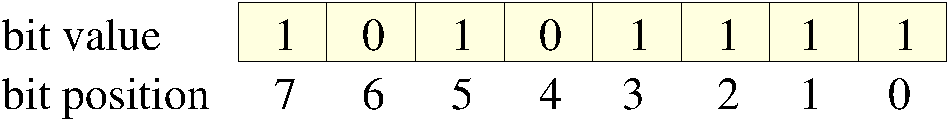
\includegraphics[width=0.6\textwidth]{175.pdf}
\end{figure}

The conversion from binary to decimal is straightforward. \index{decimal number!to binary}
It takes a little more ingenuity to convert from decimal to binary.
Let's examine the number 741.
The highest power of 2 less than (or equal to) 741 is $2^9 = 512$.
So we have 
\begin{align*}
 741 &= 512 + 229\\
     &= 2^9 + 229
\end{align*}

Now we need to work on 229.
The highest power of 2 less than 229 is $2^7 = 128$.
So we now have
\begin{align*}
741 &= 512 + 128 + 101 \\
    &= 2^9 + 2^7 + 101
\end{align*}

The process continues with 101.
The highest power of 2 less than 101 is $2^6 = 64$.
So we get
\begin{align*}
741 &= 512 + 128 + 64 + 37 \\
    &= 2^9 + 2^7 + 2^6 + 37
\end{align*}

Next we can find that 37 is greater than $2^5 = 32$, so
\begin{align*}
741 &= 512 + 128 + 64 + 32 + 5 \\
    &= 2^9 + 2^7 +2^6 + 2^5 + 5
\end{align*}

Working on the 5 we see that
\begin{align*}
741 &= 512 + 128 + 64 + 32 + 4 + 1 \\
    &= 2^9 + 2^7 +2^6 + 2^5 + 2^2 + 1 \\
    &= 1011100101
\end{align*}

Below is 741 expressed as a 16 bit integer.
\begin{figure}[h!]
\centering\includegraphics[width=0.95\textwidth]{741.pdf}
\end{figure}

A binary constant can be represented in the {\tt yasm} assembler by appending \index{binary constant}
``b'' to the end of a string of 0's and 1's.
So we could represent 741 as {\tt 1011100101b}.

An alternative method for converting a decimal number to binary is by repeated division \index{decimal number!to binary}
by 2.
At each step, the remainder yields the next higher bit.

Let's convert 741 again.  

\begin{center}
\begin{tabular}{rclcr}
\multicolumn{3}{c}{division} & remainder & bits \\
\hline
741/2 &=& 370 & 1 & 1 \\
370/2 &=& 185 & 0 & 01 \\
185/2 &=& 92  & 1 & 101 \\
92/2  &=& 46  & 0 & 0101 \\
46/2  &=& 23  & 0 & 00101 \\
23/2  &=& 11  & 1 & 100101 \\
11/2  &=& 5   & 1 & 1100101 \\
5/2   &=& 2   & 1 & 11100101 \\
2/2   &=& 1   & 0 & 011100101 \\
1/2   &=& 0   & 1 & 1011100101 \\
\end{tabular}
\end{center}

The repeated division algorithm is easier since you don't have to identify (guess?) powers of 2
less than or equal to the number under question.
It is also easy to program.

\section{Hexadecimal numbers}

Binary numbers are a fairly effective way of representing a string of bits,
but they can get pretty tedious if the string is long.
In a 64 bit computer it is fairly common to work with 64 bit integers.
Entering a number as 64 bits followed by a ``b'' would be tough.
Decimal numbers are a much more compact representation, but it is not
immediately apparent what bits are 0's and 1's in a decimal number.
Enter hexadecimal\ldots

A hexadecimal number is a number in base 16.
So we need ``digits'' from 0 to 15.
The digits from 0-9 are just like in decimal.
The digits from 10-15 are represented by the letters {\tt 'A'} through
{\tt 'F'}.  We can also use lower case letters.
Fortunately both {\tt yasm} and {\tt C/C++} represent hexadecimal numbers
using the prefix {\tt 0x}.
You could probably use {\tt 0X} but the lower case {\tt x} tends to make the
numbers more visually obvious.

Let's consider the value of {\tt 0xa1a}.
This number uses {\tt a} which means 10, so we have
\begin{align*}
{\tt 0xa1a} &= 10*16^2 + 1*16 + 10 \\
           &= 10*256 + 16 + 10 \\
           &= 2586
\end{align*}

Converting a decimal number to hexadecimal follows a pattern like the one used
before for binary numbers except that we have to find the highest power of 16
and divide by that number to get the correct ``digit''.
Let's convert 40007 to hexadecimal.
The first power of 16 to use is $16^3 = 4096$.
$40007/4096 = 9$ with a remainder of $3143$, so we have
$$40007 = 9*16^3 + 3143$$
$3143/16^2 = 3143/256 = 12$ with a remainder of $71$, so we get
$$40007 = 9*16^3 + 12*16^2 + 71$$
$71/16 = 4$ with a remainder of 7, so the final result is
$$40007 = 9*16^3 + 12*16^2 + 4*16 + 7 = {\tt 0x9c47}$$

As with conversion to binary we can perform repeated division and build the number by
keeping the remainders.

\begin{center}
\begin{tabular}{rclcr}
\multicolumn{3}{c}{division} & remainder & hex \\
\hline
40007/16 &=& 2500 & 7 & {\tt 7} \\
2500/16  &=& 156  & 4 & {\tt 47} \\
156/16   &=& 9    & 12 & {\tt c47} \\
9/16     &=& 0    & 9  & {\tt 9c47} \\
\end{tabular}
\end{center}

Converting back and forth between decimal and binary or decimal and
hexadecimal is a bit painful.
Computers can do that quite handily, but why would you want to convert from
decimal to hexadecimal?
If you are entering a value in the assembler, simply enter it in the form
which matches your interpretation.
If you're looking at the number 1027 and need to use it in your program, enter
it as a decimal number.
If you want to represent some pattern of bits in the computer, then your
choices are binary and hexadecimal.
Binary is pretty obvious to use, but only for fairly short binary strings.
Hexadecimal is more practical for longer binary strings.

The bottom line is conversion between binary and hexadecimal is all that
one normally needs to do.
This task is made easier since each hexadecimal ``digit'' represents exactly 4
bits (frequently referred to as a ``nibble'').
Consult the table below to convert between binary and hexadecimal.
\begin{center}
\begin{tabular}{|c|c|}
\hline
Hex & Binary \\
\hline
0   & 0000 \\
\hline
1   & 0001 \\
\hline
2   & 0010 \\
\hline
3   & 0011 \\
\hline
4   & 0100 \\
\hline
5   & 0101 \\
\hline
6   & 0110 \\
\hline
7   & 0111 \\
\hline
8   & 1000 \\
\hline
9   & 1001 \\
\hline
a   & 1010 \\
\hline
b   & 1011 \\
\hline
c   & 1100 \\
\hline
d   & 1101 \\
\hline
e   & 1110 \\
\hline
f   & 1111 \\
\hline
\end{tabular}
\end{center}

Let's now consider converting {\tt 0x1a5b} to binary.
1 = {\tt 0001}, {\tt a = 1010}, {\tt 5 = 0101} and {\tt b = 1011}, so we get

\begin{center}
{\tt 0x1a5b = 0001 1010 0101 1011 = 0001101001011011b}
\end{center}

Below {\tt 0x1a5b} is shown with each bit position labeled:

\begin{figure}[h!]
\centering\includegraphics[width=0.95\textwidth]{1a5b.pdf}
\end{figure}

\section{Integers}

On the x86-64 architecture integers can be 1 byte, 2 bytes, 4 bytes, or 8
bytes in length.
Furthermore for each length the numbers can be either signed or unsigned.
Below is a table listing minimum and maximum values for each type of integer.

\begin{center}
\begin{tabular}{|c|c|c|c|c|}
\hline
Variety & Bits & Bytes & Minimum & Maximum \\
\hline
unsigned & 8   & 1     & 0       & 255 \\
\hline
signed & 8     & 1     & -128    & 127 \\
\hline
unsigned & 16  & 2     & 0       & 65535 \\
\hline
signed & 16    & 2     & -32768  & 32767 \\
\hline
unsigned & 32  & 4     & 0       & 4294967295 \\
\hline
signed & 32    & 4     & -2147483648    & 2147483647 \\
\hline
unsigned & 64  & 8     & 0       & 18446744073709551615 \\
\hline
signed & 64    & 8     & -9223372036854775808    & 9223372036854775807 \\
\hline
\end{tabular}
\end{center}

The range of 64 bit integers is large enough for most needs.
Of course there are exceptions, like $20! = 51090942171709440000$.

Unsigned integers are precisely the binary numbers discussed earlier.
Signed integers are stored in a useful format called ``two's complement''.
The first bit of a signed integer is the sign bit.
If the sign bit is 0, the number is positive.
If the sign bit is 1, the number is negative.
The most obvious way to store negative numbers would be to use the remaining
bits to store the absolute value of the number.

\begin{figure}[h!]
\centering\includegraphics[width=0.95\textwidth]{signed.pdf}
\end{figure}

Let's consider 8 bit signed integers and what we would get if we used the
existing circuitry to add 2 such integers.
Let's add -1 and 1.
Well, if we store -1 with a sign bit and then the value we would get
\begin{verbatim}
       -1  =  1000 0001
        1  =  0000 0001
     ----     ---------
     -1+1  =  1000 0002
\end{verbatim}
Oops!  We end up with -2 rather than 0.

Let's try storing 8 bit numbers as a sign bit and invert the bits for 
the absolute value part of the number:
\begin{verbatim}
       -1  =  1111 1110
        1  =  0000 0001
     ----     ---------
     -1+1  =  1111 1111
\end{verbatim}
Now this is interesting: the result is actually -0, rather than 0.
This sounds somewhat hopeful.
Let's try a different pair of numbers:
\begin{verbatim}
       -1  =  1111 1110
        4  =  0000 0100
     ----     ---------
     -1+4  =  0000 0010  =  2
\end{verbatim}
Too bad!  It was close.  What we need it to add one to the complemented
absolute value for the number.
This is referred to as ``two's complement'' arithmetic.
It works out well using the same circuitry as for unsigned numbers and is
mainly a matter of interpretation.

So let's convert -1 to its two's complement format.
\begin{verbatim}
        -1   1 for the sign bit
             0000001 for the absolute value
             1111110 for the complement
             1111111 after adding 1 to the complement
        -1 = 11111111 after prefixing the sign bit
\end{verbatim}

Using two's complement numbers the largest negative 8 bit integer is
{\tt 10000000}.  To convert this back, complement the rightmost 7 bits and add
1.  This gives {\tt 1111111 + 1 = 10000000 = 128}, so {\tt 10000000 = -128}.
You may have noticed in the table of minimum and maximums that the minimum
values were all 1 larger in absolute value than the maximums.
This is due to complementing and adding 1.
The complement yields a string of 1's and adding 1 to that yields a single 1
with a bunch of 0's.
The result is that the largest value for an $n$-bit signed integer is
$2^{n-1}-1$ and the smallest value is $-2^{n-1}$.

Now let's convert the number -750 to a signed binary number.
$$750 = 512 + 128 + 64 + 32 + 8 + 4 + 2 = {\tt 1011101110b}$$
Now expressing this as a 15 bit binary number (with spaces to help keep track
of the bits) we get {\tt 000 0010 1110 1110}.
Next we invert the bits to get {\tt 111 1101 0001 0001}.
Finally we add 1 and prefix the number with the sign bit to get
{\tt -750 = 1111 1101 0001 0010 = 0xFD12}.

Next let's convert the hexadecimal value {\tt 0xFA13} from a 16 bit signed
integer to a decimal value.
Start by converting the rightmost 15 bits to binary: {\tt 111 1010 0001 0011}.
Then invert the bits: {\tt 000 0101 1110 1100}.
Add 1 to get the 2's complement: {\tt 000 0101 1110 1101}.
Convert this to decimal $1024 + 256 + 128 + 64 + 32 + 8 + 4 + 1 = 1517$,
so {\tt 0xFA13 = -1517}.

Let's add -750 and -1517 in binary:
\begin{verbatim}
           1111 1101 0001 0010
           1111 1010 0001 0011
           -------------------
         1 1111 0111 0010 0101
\end{verbatim}
We can ignore the leading 1 bit (a result of a carry).
The 16 bit sum is {\tt 1111 0111 0010 0101}, which is negative.
Inverting the lowermost 15 bits: {\tt 0000 1000 1101 1010}.
Next adding 1 to get the two's complement: {\tt 0000 1000 1101 1011}.
So the number is $2048 + 128 + 64 + 16 + 8 + 2 + 1 = 2267$.
So we have $-750 + -1517 = -2267$.

\subsection{Binary addition}

Performing binary addition is a lot like decimal addition.
Let's add 2 binary numbers

\begin{center}
\begin{tabular}{cr}
         & {\tt 10101111} \\
 {\tt +} & {\tt 11010010} \\
\hline
         & {\tt 1}
\end{tabular}
\end{center}

The first pair of bits was easy.
Adding the second pair of bits gives a value of 2, but 2 = {\tt 10b}, so we
place a 0 on the bottom and carry a 1

\begin{center}
\begin{tabular}{cr}
         & {\tt 1\ \ } \\
         & {\tt 10001111} \\
 {\tt +} & {\tt 01011010} \\
\hline
         & {\tt 01}
\end{tabular}
\end{center}

We continue in the same way:

\begin{center}
\begin{tabular}{cr}
         & {\tt 1\ \ \ } \\
         & {\tt 10001111} \\
 {\tt +} & {\tt 01011010} \\
\hline
         & {\tt 001}
\end{tabular}
\end{center}

\begin{center}
\begin{tabular}{cr}
         & {\tt 1\ \ \ \ } \\
         & {\tt 10001111} \\
 {\tt +} & {\tt 01011010} \\
\hline
         & {\tt 1001}
\end{tabular}
\end{center}

\begin{center}
\begin{tabular}{cr}
         & {\tt 1\ \ \ \ \ } \\
         & {\tt 10001111} \\
 {\tt +} & {\tt 01011010} \\
\hline
         & {\tt 01001}
\end{tabular}
\end{center}

\begin{center}
\ldots
\end{center}

\begin{center}
\begin{tabular}{cr}
         & {\tt 10001111} \\
 {\tt +} & {\tt 01011010} \\
\hline
         & {\tt 11101001}
\end{tabular}
\end{center}

\subsection{Binary multiplication}

Binary multiplication is also much like decimal multiplication.
You multiply one bit at a time of the second number by the top number and write these
products down staggered to the left.
Of course these ``products'' are trivial.
You are multiplying by either 0 or 1.
In the case of 0, you just skip it.
For 1 bits, you simply copy the top number in the correct columns.

After copying the top number enough times, you add all the partial products.
Here is an example:

\begin{center}
\begin{tabular}{cr}
       & {\tt 1010101} \\
    *  & {\tt 10101} \\
\hline
       & {\tt 1010101} \\
       & {\tt 1010101\ \ } \\
       & {\tt 1010101\ \ \ \ } \\
\hline
       & {\tt 11011111001}
\end{tabular}
\end{center}


\section{Floating point numbers}

The x86-64 architecture supports 3 different varieties of floating point
numbers: 32 bit, 64 bit and 80 bit numbers.
These numbers are stored in IEEE 754 format.
Below are the pertinent characteristics of these types

\begin{center}
\begin{tabular}{|l|c|c|c|c|c|}
\hline
Variety & Bits & Exponent & Exponent Bias & Fraction & Precision \\
\hline
float   &  32  & 8        &   127         & 23       & $\sim$7 digits \\
\hline
double  &  64  & 11       &  1023         & 52       & $\sim$16 digits \\
\hline
long double & 80 & 15     & 16383         & 64       & 19 digits \\
\hline
\end{tabular}
\end{center}

The IEEE format treats these different length numbers in the same way, but
with different lengths for the fields.
In each format the highest order bit is the sign bit.
A negative number has its sign bit set to 1 and the remaining bits are just
like the corresponding positive number.
Each number has a binary exponent and a fraction.
We will focus on the {\tt float} type to reduce the number of bits involved.
\begin{figure}[h!]
\centering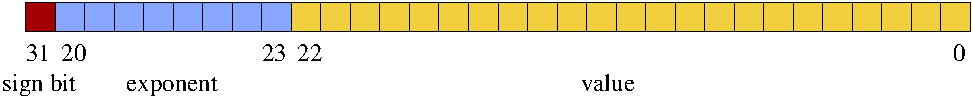
\includegraphics[width=0.95\textwidth]{float.pdf}
\end{figure}

The exponent for a float is an 8 bit field.
To allow large numbers or small numbers to be stored, the exponent is
interpreted as positive or negative.
The actual exponent is the value of the 8 bit field minus 127.
127 is the ``exponent bias'' for 32 bit floating point numbers.

The fraction field of a {\tt float} has a small surprise.
Since 0.0 is defined as all bits set to 0, there is no need to worry about
representing 0.0 as an exponent field equal to 127 and fraction field set to
all 0's.
All other numbers have at least one 1 bit, so
the IEEE 754 format uses an implicit 1 bit to save space.
So if the fraction field is {\tt 00000000000000000000000}, it is interpreted
as {\tt 1.00000000000000000000000}. 
This allows the fraction field to be effectively 24 bits.
This is a clever trick made possible by making exponent fields of {\tt 0x00}
and {\tt 0xFF} special.

A number with exponent field equal to {\tt 0x00} is defined to be 0.
Interestingly, it is possible to store a negative 0.
An exponent of {\tt 0xFF} is used to mean either negative or positive
infinity.
There are more details required for a complete description of IEEE 754,
but this is sufficient for our needs.

To illustrate floating point data, consider the following assembly file \index{segment!.data}
\begin{verbatim}
        segment .data
zero    dd      0.0
one     dd      1.0
neg1    dd      -1.0
a       dd      1.75
b       dd      122.5
d       dd      1.1
e       dd      10000000000.0
\end{verbatim}
This is not a program, it is simply a definition of 7 {\tt float} values
in the {\tt .data} segment.
The {\tt dd} command specifies a double word data item.
Other options include {\tt db} (data byte), {\tt dw} (data word) and
{\tt dq} (data quad-word).
A word is 2 bytes, a double word is 4 bytes and a quad-word is 8 bytes.

Now consider the listing file produced by {\tt yasm}
\begin{verbatim}
1                                 %line 1+1 fp.asm
2                                 [section .data]
3 00000000 00000000               zero dd 0.0
4 00000004 0000803F               one dd 1.0
5 00000008 000080BF               neg1 dd -1.0
6 0000000C 0000E03F               a dd 1.75
7 00000010 0000F542               b dd 122.5
8 00000014 CDCC8C3F               d dd 1.1
9 00000018 F9021550               e dd 10000000000.0
\end{verbatim}

The {\tt zero} variable is stored as expected - all 0 bits.
The other numbers might be a little surprising.
Look at {\tt one} - the bytes are backwards!
Reverse them and you get {\tt 3F800000}.
The most significant byte is {\tt 3F}.  The sign bit is 0.
The exponent field consists of the other 7 bits of the most significant byte
and the first bit of the next byte.
This means that the exponent field is 127 and the actual binary exponent is 0.
The remaining bits are the binary fraction field - all 0's.
Thus the value is $1.0 * 2^0 = 1.0$.

There is only 1 negative value shown: -1.0.
It differs in only the sign bit from 1.0.

You will notice that 1.75 and 122.5 have a significant number of 0's in the
fraction field.
This is because .75 and .5 are both expressible as sums of negative powers of
2.
$$0.75 = 0.5 + 0.25 = 2^{-1} + 2^{-2}$$
On the other hand 1.1 is a repeating sequence of bits when expressed in
binary.
This is somewhat similar to expressing 1/11 in decimal:
$$1/11 = 0.090909\cdots$$
Looking at 1.1 in the proper order {\tt 1.1 = 0x3F8CCCCD}.
The exponent is 0 and the fraction field in binary is
{\tt 00011001100110011001101}.
It looks like the last bit has been rounded up and that the repeated pattern
is {\tt 1100}.
$$1.1_{10} = 1.00011001100110011001100\cdots_2$$

Having seen that floating point numbers are backwards, then you might suspect
that integers are backwards also.
This is indeed true.
Consider the following code which defines some 32 bit integers
\begin{verbatim}
        segment data
zero    dd      0
one     dd      1
neg1    dd      -1
a       dd      175
b       dd      4097
d       dd      65536
e       dd      100000000
\end{verbatim}

The associated listing file shows the bits generated for each number.
The bytes are backwards.  Notice that 4097 is represented as {\tt 0x01100000}
in memory.
The first byte is the least significant byte.
We would prefer to consider this as {\tt 0x00001001}, but the CPU stores least
significant byte first.

\begin{verbatim}
1                                 %line 1+1 int.asm
2                                 [section .data]
3 00000000 00000000               zero dd 0
4 00000004 01000000               one dd 1
5 00000008 FFFFFFFF               neg1 dd -1
6 0000000C AF000000               a dd 175
7 00000010 01100000               b dd 4097
8 00000014 00000100               d dd 65536
9 00000018 00E1F505               e dd 100000000
\end{verbatim}

\subsection{Converting decimal numbers to floats}

Let's work on an example to see how to do the conversion.
Let's convert -121.6875 to decimal.

First let's note that the sign bit is 1.
Now we will work on 121.6875.

It's fairly easy to convert the integer portion of the number: 121 = {\tt 1111001b}.
Now we need to work on the fraction.

Let's suppose we have a binary fraction $x$ = {\tt 0.abcdefgh}, where the letters indicate either a 0 or a 1.
Then 2*$x$ = {\tt a.bcdefgh}.
This indicates that multiplying a fraction by 2 will expose a bit.

We have $2 \times 0.6875 = 1.375$ so the first bit to the right of the binary point is 1.
So far our number is {\tt 1111001.1b}.

Next multiply the next fraction: $2 \times 0.375 = 0.75$, so the next bit is 0.
We have {\tt 1111001.10b}

Multiplying again: $2 \times 0.75 = 1.5$, so the next bit is 1.
We now have {\tt 1111001.101b}.

Multiplying again: $2 \times 0.5 = 1$, so the last bit is 1.
We have {\tt 1111001.1011b}

So our number -121.6875 = {\tt -1111001.1011b}.
We need to get this into exponential notation with a power of 2.

\begin{center}
\begin{align*}
  -121.6875 &= -1111001.1011 \\
            &= -1.1110011011 * 2^6
\end{align*}
\end{center}

We now have all the pieces.
The sign bit is 1, the fraction (without the implied 1) is {\tt 11100110110000000000000} and the exponent field
is 127+6 = 133 = {\tt 10000101}.
So our number is {\tt 1 10000101 11100110110000000000000}.
Organized into nibbles, this is {\tt 1100 0010 1111 0011 0110 0000 0000 0000} or {\tt 0xc2f36000}.
Of course if you see this in a listing it will be reversed: {\tt 0060f3c2}.

\subsection{Converting floats to decimal}

An example will illustrate how to convert a float to a decimal number.
Let's work on the float value {\tt 0x43263000}.

The sign bit is 0, so the number is positive.
The exponent field is {\tt 010000110} which is 134, so the binary exponent is 7.
The fraction field is {\tt 010 0110 0011 0000 0000 0000 0000}, so the fraction with implied 1 is
{\tt 1.01001100011}.
\begin{center}
 \begin{align*}
  1.01001100011_2 * 2^7 &= 10100110.0011_2 \\
                     &= 166 + 2^{-3} + 2^{-4} \\
                     &= 166 + 0.125 + 0.0625 \\
                     &= 166.1875
 \end{align*}

\end{center}

\subsection{Floating point addition}

In order to add two floating point numbers, we must first convert the numbers to binary real numbers.
Then we need to align the binary points and add the numbers.
Finally we need to convert back to floating point.

Let's add the numbers 41.275 and 0.315.
In hexadecimal these numbers are {\tt 0x4225199a} and {\tt 0x3ea147ae}.
Now let's convert {\tt 0x4225199a} to a binary number with a binary exponent.
The exponent field is composed of the first two nibbles and a 0 bit from the next nibble.
This is ${\tt 10000100}_2 = 132$, so the exponent is $132-127=5$.
The fractional part with the understood 1 bit is
$$1.01001010001100110011010_2$$.
So we have
\begin{align*}
{\tt 0x4225199a} &= 1.01001010001100110011010_2 * 2^5 \\
                 &= 101001.010001100110011010_2
\end{align*}

Similarly {\tt 0x3ea147ae} has an exponent field of the first 2 nibbles and a 1 from the third nibble.
So the exponent field is ${\tt 01111101}_2 = 125$ yielding an exponent of -2.
The fractional part with the understood 1 bit is
$$1.01000010100011110101110_2$$
So we have
\begin{align*}
{\tt 0x3ea147ae} &= 1.01000010100011110101110_2 * 2^{-2} \\
                 &= 0.0101000010100011110101110_2
\end{align*}

Now we can align the numbers and add

\begin{tabular}{ll}
    & {\tt 101001.010001100110011010} \\
  + & {\tt \ \ \ \ \ 0.0101000010100011110101110}\\
  \hline
    & {\tt 101001.1001011100001010010101110}
\end{tabular}

Now we have too many bits to store in a 32 bit float.
The rightmost 7 bits will be rounded (dropped in this case) to get
\begin{align*}
    & {\tt 101001.100101110000101001}_2 \\
  = & {\tt 1.01001100101110000101001}_2 * 2^5
\end{align*}

So the exponent is 5 and the exponent field is again 132.
Dropping the leading 0, we get {\tt 0x42265c29} which is 41.59 (approximately).

You should be able to see that we lost some bits of precision on the smaller number.
In an extreme case we could try to add 1.0 to a number like $10^{38}$ and have no effect.

\subsection{Floating point multiplication}

Floating point multiplication can be performed in binary much like decimal multiplication.
Let's skip the floating point to/from binary conversion and just focus on the multiplication of
7.5 and 4.375.

\begin{center}
\begin{tabular}{crcr}
   &  7.5 & = & ${\tt 111.1}_2$ \\ 
 * &  4.375 & = & ${\tt 100.011}_2$ \\
    \hline
   &       &   & ${\tt 1111}_2$ \\
   &       &   & ${\tt 11110}_2$ \\
   &       &   & ${\tt 111100000}_2$ \\
   \hline
    &       &   & ${\tt 100000.1101}_2$
\end{tabular}
\end{center}


\vfill
\break
{\bf\large Exercises}

\begin{enumerate}

\item Convert the following integers to binary.

\begin{tabular}{p{2in}p{2in}}
a. 37    & -65 \\
b. 350   & -427
\end{tabular}

\item Convert the following 16 bit signed integers to decimal.

\begin{tabular}{p{2in}p{2in}}
a. {\tt 0000001010101010b}    & c. {\tt 0x0101} \\
b. {\tt 1111111111101101b}    & d. {\tt 0xffcc} \\
\end{tabular}

\item Convert the following 16 bit unsigned integers to binary.

\begin{tabular}{p{2in}p{2in}}
a. {\tt 0x015a}    & c. {\tt 0x0101} \\
b. {\tt 0xfedc}    & d. {\tt 0xacdc} \\
\end{tabular}

\item Convert the following numbers to 32 bit floating point.

\begin{tabular}{p{2in}p{2in}}
a. 1.375    & c. -571.3125 \\
b. 0.041015625    & d. 4091.125 \\
\end{tabular}

\item Convert the following numbers from 32 bit floating point to decimal.

\begin{tabular}{p{2in}p{2in}}
a. {\tt 0x3F82000}    & c. {\tt 0x4F84000} \\
b. {\tt 0xBF82000}    & d. {\tt 0x3C86000} \\
\end{tabular}

\item Perform the binary addition of 2 unsigned integers below.  Show each
carry as a 1 above the proper position.

\begin{verbatim}
       0001001011001011
      +1110110111101011
      -----------------
\end{verbatim}

\item Perform the binary multiplication of the following unsigned binary numbers.  Show each row where a 1 is multiplied times the top number.
You may omit rows where a 0 is multiplied times the top number.

\begin{verbatim}
           1011001011
      *       1101101
      ---------------
\end{verbatim}


\item Write an assembly ``program'' (data only) defining data values using
{\tt dw} and {\tt dd} for all the numbers in exercises 1-4.

\end{enumerate}

\chapter{Computer memory}

In this chapter we will discuss how a modern computer performs memory mapping
to give each process a protected address space and how the Linux system
manages the memory for a process.
A practical benefit of this chapter is a discussion of how to examine memory
using the {\tt gdb} debugger.

\section{Memory mapping}

The memory of a computer can be considered an array of bytes.
Each byte of memory has an address.
The first byte is at address 0, the second byte at address 1, and so on
until the last byte of the computer's memory.

In modern CPUs there are hardware mapping registers which
are used to give each process a protected address space.
This means that multiple people can each run a program which starts at
address {\tt 0x4004c8} at the same time.
These processes perceive the same ``logical'' addresses, while they are
using memory at different ``physical'' addresses.

The hardware mapping registers on an x86-64 CPU can map pages of 2 different
sizes - 4096 bytes and 2 megabytes.
Linux uses 2 MB pages for the kernel and 4 KB pages for most other uses.
In some of the more recent CPUs there is also support for 1 GB pages.

The operation of the memory system is to translate the upper bits of the
address from a process's logical address to a physical address.
Let's consider only 4 KB pages.
Then an address is translated based on the page number and the address
within the page.
Suppose a reference is made to logical address {\tt 0x4000002220}.
Since $4096 = 2^{12}$, the offset within the page is the right-most
12 bits ({\tt 0x220}).
The page number is the rest of the bits ({\tt 0c=x4000002}).
A hardware register (or multiple registers) translates this page number to
a physical page address, let's say {\tt 0x780000000}.
Then the two addresses are combined to get the physical address
{\tt 0x780000220}.

Amazingly the CPU generally performs the translations without slowing down
and this benefits the users in several ways.
The most obvious benefit is memory protection.
User processes are limited to reading and writing only their own pages.
This means that the operating system is protected from malicious or poorly
coded user programs.
Also each user process is protected from other user processes.
In addition to protection from writing, users can't read other users' data.

There are instructions used by the operating system to manage the hardware
mapping registers.
These instructions are not discussed in this book.
Our focus is on programming user processes.

So why bother to discuss paging, if we are not discussing the instructions to
manage paging?
Primarily this improves one's understanding of the computer.
When you write software which accesses data beyond the end of an array, you
sometimes get a segmentation fault.
However you only get a segmentation fault when your logical address reaches
far enough past the end of the array to cause the CPU to reference a page
table entry which is not mapped into your process.

\section{Process memory model in Linux}

In Linux memory for a process is divided into 4 logical regions: text, data,
heap and stack.
The stack is mapped to the highest address of a process and on x86-64 Linux
this is {\tt 0x7fffffffffff} or 131 TB.
This address is selected based on the maximum number of bits allowed in
logical addresses being 48 bits.
This address is 47 bits of all 1 bits.
The decision was made to not use bit 48, since canonical addresses have to
extend bit 48 through bits 49-63.

\begin{wrapfigure}{r}{1.3in}
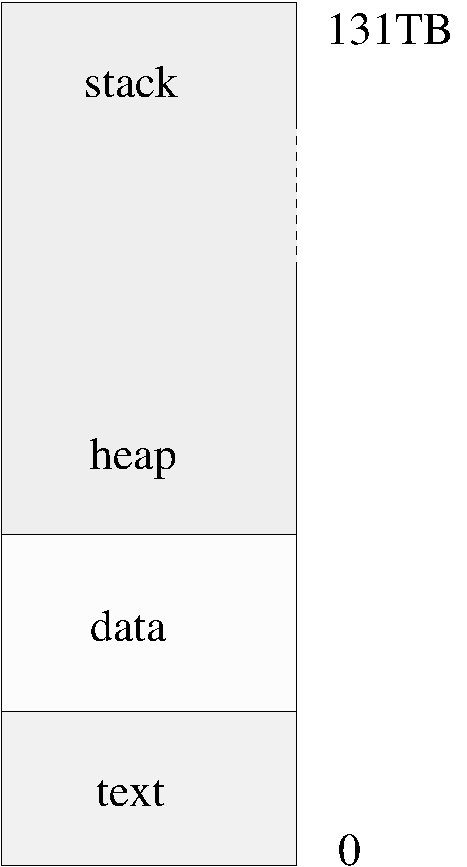
\includegraphics[width=1.3in]{process_memory.pdf}
\caption{Process memory layout}
\label{process:memory}
\end{wrapfigure}

In figure \ref{process:memory} we see the arrangement of the various memory
segments.
At the lowest address we have the text segment ({\tt .text} for {\tt yasm}).
This segment is shown starting at 0, though both {\tt \_start} and {\tt main} are at
higher addresses.
It appears that the lowest address in an x86-64 process is {\tt 0x400000}.
The text segment does not typically need to grow, so the data segment is
placed immediately above the text segment.
Above these two segments are the heap and stack segments.

The data segment starts with the {\tt .data} segment which contains \index{segment!.data}
initialized data.
Above that is the {\tt .bss} segment which stands for ``block started by \index{segment!.bss}
symbol''.
The {\tt .bss} segment contains data which is statically allocated in a
process, but is not stored in the executable file.
Instead this data is allocated when the process is loaded into memory.
The initial contents of the {\tt .bss} segment are all 0 bits.

The heap is not really a heap in the sense discussed in a data structures \index{heap}
course.
Instead is a dynamically resizable region of memory which is used to allocate
memory to a process through functions like {\tt malloc} in C and the {\tt new}
operator in C++.
In x86-64 Linux this region can grow to very large sizes.
The limit is imposed by the sum of physical memory and swap space.

The final segment of a process is the stack segment. \index{segment!stack}
This segment is restricted in size by the Linux kernel, typically to 16
megabytes.
This is not a large amount of space, but as long as the programmer avoids
putting large arrays on the stack it serves the purpose quite well of managing
the run-time stack keeping track of function calls, parameters, local
variables and return addresses.

Given the top of the stack as {\tt 0x7fffffffffff} and the stack size limited
to 16 megabytes we see that the lowest valid stack address is {\tt 0x7fffff000000}.
The stack automatically grows when needed by the operating system responding
to a page fault.
The operating system recognizes the faulting address as being in the range
from {\tt 0x7fffff000000} to {\tt 0x7fffffffffff}, which is only used for the
stack and allocates a new page of memory (4096 bytes) to the process.

This simple memory layout is not entirely accurate.
There are shared object files which can be mapped into a process after the
program is loaded which will result in regions in the heap range being used to
to store instructions and data.
This region is also used for mapping shared memory regions into a process.

If you wish to examine the memory used by one of your processes, you can
execute ``{\tt cat /proc/999/maps}'' where 999 needs to be replaced by your process id.
To see the memory used by your shell process, enter
\begin{verbatim}
        cat /proc/$$/maps
\end{verbatim}

\section{Memory example}

Here is a sample assembly program with several memory items defined:
\begin{verbatim}
        segment .data
a       dd      4
b       dd      4.4
c       times   10 dd 0
d       dw      1, 2
e       db      0xfb
f       db      "hello world", 0

        segment .bss
g       resd    1
h       resd    10
i       resb    100

        segment .text
        global  main        ; let the linker know about main
main:
        push    rbp         ; set up a stack frame for main
        mov     rbp, rsp    ; set rbp to point to the stack frame
        sub     rsp, 16     ; leave some room for local variables
                            ; leave rsp on a 16 byte boundary
        xor     eax, eax    ; set rax to 0 for return value
        leave               ; undo the stack frame manipulations
        ret
\end{verbatim}

After assembling the program we get the following listing file:
\begin{verbatim}
 1                                 %line 1+1 memory.asm
 2                                 [section .data]
 3 00000000 04000000               a dd 4
 4 00000004 CDCC8C40               b dd 4.4
 5 00000008 00000000<rept>         c times 10 dd 0
 6 00000030 01000200               d dw 1, 2
 7 00000034 FB                     e db 0xfb
 8 00000035 68656C6C6F20776F72-    f db "hello world", 0
 9 00000035 6C6400             
10                                 
11                                 [section .bss]
12 00000000 <gap>                  g resd 1
13 00000004 <gap>                  h resd 10
14 0000002C <gap>                  i resb 100
15                                 
16                                 [section .text]
17                                 [global main]
18                                 main:
19 00000000 55                      push rbp
20 00000001 4889E5                  mov rbp, rsp
21 00000004 4883EC10                sub rsp, 16
22 00000008 31C0                    xor eax, eax
23 0000000A C9                      leave
24 0000000B C3                      ret
\end{verbatim}

You can see from the listing the relative addresses of the defined data elements.
In the data section we have a double word (4 bytes) named {\tt a} at location 0.
Notice that the bytes of {\tt a} are reversed compared to what you might prefer.

Following {\tt a} is a double word defined as a floating point value
named {\tt b} at relative address 4.
The bytes for {\tt b} are also reversed.
Consider it as {\tt 0x408ccccd}.  Then the sign bit is 0, the exponent
field is the rightmost 7 bits of the ``first'' byte, {\tt 0x40}, with
the leftmost bit of the next byte, {\tt 0x8c}.
So the exponent field is {\tt 0x81} = 129, which is a binary exponent of 2.
The fraction field (with the implied initial 1 bit) is {\tt 0x8ccccd}.
So {\tt b} = {\tt 1.00011001100110011001101} $*$ $2^2$ = 4.4.

The next data item is the array {\tt c} defined with the {\tt times} pseudo-op which has 10 double word locations.
The relative location for {\tt c} is 8 and {\tt c} consists of 40 bytes, so the next item after {\tt c} is at relative address 48 or {\tt 0x30}.

Following {\tt c} is the length 2 array {\tt d} with values 1 and 2.
Array {\tt d} is of type word so each value is 2 bytes.
Again you can see that the bytes are reversed for each word of {\tt d}.

The next data item is the byte variable {\tt e} with initial value
{\tt 0xfb}.
After {\tt e} is the byte array {\tt f} which is initialized with a
string.
Notice that I have added a terminal null byte explicitly to {\tt f}.
Strings in {\tt yasm} do not end in null bytes.

After the data segment I have included a bss segment with 3 variables.
These are listed with their relative addresses as part of the bss segment.
After linking the bss data items will be loaded into memory beginning 
with {\tt g} defined by {\tt resd} op-code which means ``reserve'' double word.
With {\tt resd} the number 1 means 1 double word.
The next bss item is {\tt h} which has 10 reserved double words.
The last bss item is {\tt i} which has 100 reserved bytes.
All these data items are shown in the listing with addresses relative to the
start of the bss segment.
They will all have value 0 when the program starts.

\section{Examining memory with {\tt gdb}}

In this section we will focus on using the {\tt gdb} print ({\tt p}) and examine ({\tt x}) commands.
Print is a simple command which can print some data values and is versatile enough to print various forms of C expressions.
Examine is strictly for printing data from memory and is quite useful for
printing arrays of various types.

\subsection{Printing with {\tt gdb}}

The format for the {\tt p} command is either {\tt p expression} or \index{gdb!print}
{\tt p/FMT expression} where {\tt FMT} is a single letter defining the
format of data to print.
The format choices are
\begin{center}
\begin{tabular}{|c|l|}
\hline
letter & format \\
\hline
d      & decimal (default) \\
\hline
x 		& hexadecimal \\
\hline
t     & binary \\
\hline
u     & unsigned \\
\hline
f     & floating point \\
\hline
i     & instruction \\
\hline
c     & character \\
\hline
s     & string \\
\hline
a     & address \\
\hline
\end{tabular}
\end{center}

Let's see a few commands in action in {\tt gdb}:
\begin{verbatim}
(gdb) p a
$32 = 4
(gdb) p/a &a
$33 = 0x601018 <a>
(gdb) p b
$34 = 1082969293
(gdb) p/f b
$35 = 4.4000001
(gdb) p/a &b
$36 = 0x60101c <b>
(gdb) p/x &b
$37 = 0x60101c
(gdb) p/a &c
$39 = 0x601020 <c>
(gdb) p/a &d
$40 = 0x601048 <d>
(gdb) p/a &e
$41 = 0x60104c <e>
(gdb) p/a &f
$42 = 0x60104d <f>
(gdb) p/a &g
$43 = 0x601070 <g>
(gdb) p/a &h
$45 = 0x601074 <h>
(gdb) p/a &i
$46 = 0x60109c <i>

\end{verbatim}

We see that {\tt gdb} handles {\tt a} perfectly.
It gets the type right and the length.
It needs the {\tt /f} option to print {\tt b} correctly.
Notice that {\tt a} is located at address {\tt 0x601018} which is 24 bytes
after the start of a page in memory.
{\tt gdb} will prohibit accessing memory before {\tt a}, though there is
no hardware restriction to the previous 24 bytes.
We see that the data segment variables are placed in memory one after another until {\tt f} which starts at {\tt 0x60104d} and extends to
{\tt 0c601058}.
There is a gap until the bss segment which starts with {\tt g} at
address {\tt 0x601070}.
The bss data items are placed back to back in memory with no gaps.

\subsection{Examining memory}

Notice that there are no length specifiers with {\tt p}. \index{gdb!examine}
If you want to print doubles in memory it could be done with some mental gymnastics with {\tt p}.
The examine command handles this job readily.

The format for examine is {\tt x/NFS address} where {\tt N} is a number of items
to print (default 1), {\tt F} is a single letter format as used in the print
command and {\tt S} is the size of each memory location.
Unfortunately {\tt gdb} picked some size letters which conflict with
some of the size options in {\tt yasm}.
Here are the size options:
\begin{center}
\begin{tabular}{|c|l|c|}
\hline
letter & size & bytes \\
\hline
b      & byte & 1 \\
\hline
h 		& halfword & 2 \\
\hline
w     & word & 4 \\
\hline
g     & giant & 8 \\
\hline
\end{tabular}
\end{center}

Here are some examples of examining memory:
\begin{verbatim}
(gdb) x/w &a
0x601018 <a>:	0x4
(gdb) x/fw &b
0x60101c <b>:	4.4000001
(gdb) x/fg &b
0x60101c <b>:	5.3505792317228316e-315
(gdb) x/10dw &c
0x601020 <c>:	0	0	0	0
0x601030 <c+16>:	0	0	0	0
0x601040 <c+32>:	0	0
(gdb) x/2xh &d
0x601048 <d>:	0x0001	0x0002
(gdb) x/12cb &f
0x60104d <f>:	104 'h'	101 'e'	108 'l'	108 'l'	111 'o'	32 ' '	119 'w'	111 'o'
0x601055 <f+8>:	114 'r'	108 'l'	100 'd'	0 '\000'
(gdb) x/s &f
0x60104d <f>:	 "hello world"
\end{verbatim}

Things match what you expect if you use the correct format and size.
I first printed {\tt b} with the correct size and then with the giant size (8 bytes).
{\tt gdb} interpreted 8 bytes of memory starting at the address of {\tt b} 
as a double getting the wrong exponent and fraction.
The use of the count field is quite useful for dumping memory.

\vfill
\break
{\bf\large Exercises}

\begin{enumerate}
 \item Write a data-only program like the one in this chapter to define an array of 10 8 byte integers
 in the data section, an array of 5 2 byte integers in the bss section, and a string terminated by 0 in the 
 data section.
 Use {\tt gdb}'s examine command to print the 8 byte integers in hexadecimal, the 2 byte integers as unsigned
 values, and the string as a string.
 \item Assuming that the stack size limit is 16MB, about how large can you declare an array of {\tt double}s inside
 a C++ function.  Do not use the keyword {\tt static}.
 \item Find out the stack size limit using the {\tt ulimit} command in bash.  If bash is not your shell, simply
 type in {\tt bash} to start a sub-shell.
 \item Print the value of {\tt rsp} in {\tt gdb}.  How many bits are required to store this value?
\end{enumerate}

\chapter{Memory mapping in 64 bit mode}

In this chapter we discuss the details of how virtual addresses are translated to
physical addresses in the x86-64 architecture.\index{virtual address} \index{physical address}
Some of the data for translation is stored in the CPU and some of it is stored
in memory.

\section{The memory mapping register}

Well the CPU designers named this register ``Control Register 3'' or just CR3.
A simplified view of CR3 is that it is a pointer to the top level of a hierarchical collection of tables in memory which define the translation \index{CR3}
from virtual addresses (the addresses your program sees) to physical addresses.
The CPU retains quite a few page translations internally, but let's consider
first how the CPU starts all this translation process.

Somewhere in the kernel of the operating system, an initial hierarchy of the
translation tables is prepared and CR3 is filled with the address of the
top level table in the hierarchy.
This table is given the illustrious name ``Page Map Level 4'' or PML4. \index{PML4}
When the CPU is switched to using memory mapping on the next memory reference it
starts by using CR3 to fetch the address of PML4.
Surely it must retain PML4's address for future use.

\section{Page Map Level 4}

A virtual address can be broken into fields like this:

\begin{center}
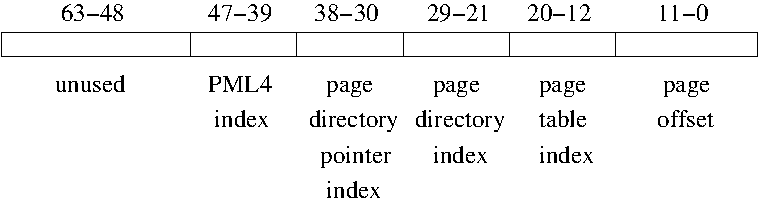
\includegraphics[width=0.95\textwidth]{address.pdf}
\end{center}

Here we see that a virtual or logical address is broken into 6 fields.
The top-most 16 bits are ignored.
They are supposed to be a sign extension of bit 47,
but they are not part of the address translation.
Following the unused bits are four 9 bit fields which undergo translation
and finally a 12 bit page offset.
The result of the translation process will be a physical address like
{\tt 0x7fffff008000} which is combined with the offset (let's say it was {\tt 0x1f0} to yield a physical address of {\tt 0x7fffff0081f0}.

Pages of memory are $2^{12}=4096$ bytes, so the 12 bit offset makes sense.
What about those 9 bit fields?
Well, addresses are 8 bytes so you can store 512 addresses in a page and
$512=2^9$, so 9 bit fields allow storing each of the 4 types of mapping
tables in a page of memory.

Bits 47-39 of a virtual address as used as an index into the PML4 table.
The PML4 table is essentially an array of 512 pointers.
These pointers point to pages of memory, so the rightmost 12 bits of each
pointer can be used for other purposes like indicating whether an entry is
valid or not.
Generally not all entries in the PML4 will be valid.\index{PML4}

Let's suppose that CR3 has the physical address {\tt 0x4ffff000}.
Then let's suppose that bits 47-39 of our sample address are {\tt 0x001},
then we would have an array in memory at {\tt 0x4ffff000} and we would
access the second entry (index 1) to get the address of a page directory
pointer table - {\tt 0x3467000}. \index{page directory pointer table}

\begin{center}
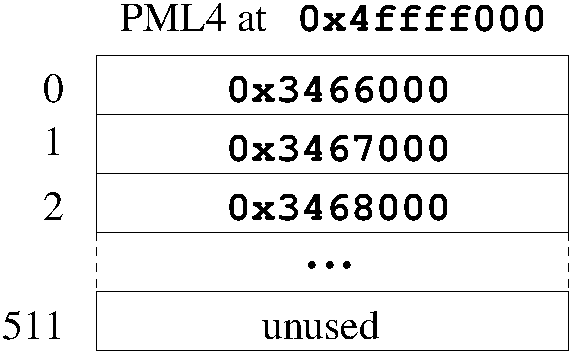
\includegraphics[width=0.35\textwidth]{pml4.pdf}
\end{center}

\section{Page Directory Pointer Table}

The next level in the memory translation hierarchy is the collection
of page directory pointer tables.
Each of these tables is also an array of 512 pointers.
These pointers are to page directory tables.
Let's assume that our sample address has the value {\tt 0x002} for bits
38-30.
Then the computer will fetch the third entry of the page directory pointer
table to lead next to a page directory table at address {\tt 0x3588000}.
\index{page directory table}

\begin{center}
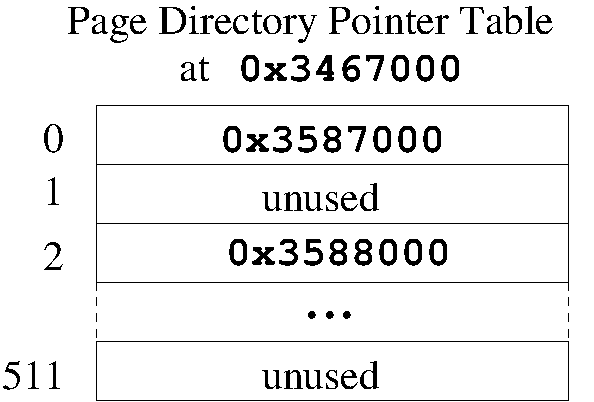
\includegraphics[width=0.35\textwidth]{pdptable.pdf}
\end{center} \index{page directory pointer table}

\section{Page Directory Table}

The third level in the memory translation hierarchy is the collection
of page directory tables.
Each of these tables is also an array of 512 pointers,
which point to page tables.
Let's assume that our sample address has the value {\tt 0x000} for bits
29-21.
Then the computer will fetch the first entry of the page directory
table to lead next to a page table at address {\tt 0x3678000}.
\index{page directory table} \index{page table}
\begin{center}
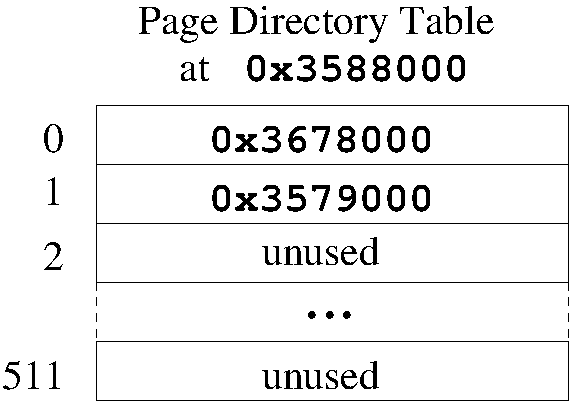
\includegraphics[width=0.35\textwidth]{pdtable.pdf}
\end{center}
\section{Page Table}

The fourth and last level in the memory translation hierarchy is the collection
of page tables.
Again each of these tables is an array of 512 pointers to pages.
Let's assume that our sample address has the value {\tt 0x1ff} for bits
20-12.
Then the computer will fetch the first entry of the page directory pointer
table to lead next to a page table at address {\tt 0x5799000}.
\begin{center}
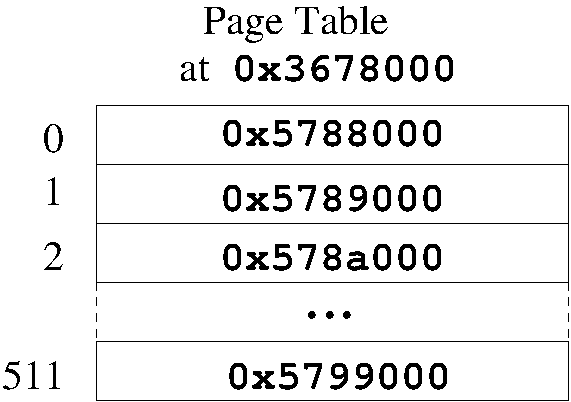
\includegraphics[width=0.35\textwidth]{ptable.pdf}
\end{center}  
\index{page table}

After using 4 tables we reach the address of the page of memory which was
originally referenced.
Then we can or in the page offset (bits 11-0) of the original - say {\tt 0xfa8}.
This yields a final physical address of {\tt 0x5799fa8}.
\index{physical address}

\section{Large pages}

The normal size page is 4096 bytes. \index{large page}
The CPU designers have added support for large pages using three levels of
the existing translation tables.
By using 3 levels of tables, there are $9+12=21$ bits left for the within page
offset field.
This makes large pages $2^{21}= 2097152$ bytes.

\section{CPU Support for Fast Lookups}

This process would be entirely too slow if done every time by traversing through
all these tables. \index{translation lookaside buffer} \index{TLB}
Instead whenever a page translation has been performed, the CPU adds this translation into a cache called a ``Translation Lookaside Buffer'' or TLB.
Then hopefully this page will be used many times without going back through the
table lookup process.

A TLB operates much like a hash table.
It is presented with a virtual page address and produces a physical page address
or failure within roughly $1/2$ of a clock cycle.
In the case of a failure the memory search takes from 10 to 100 cycles.
Typical miss rates are from 0.01\% to 1\%.


Clearly there is a limit to the number of entries in the TLB for a CPU.
The Intel Core 2 series has a total of 16 entries in a level 1 TLB and 
256 entries in a level 2 TLB.
The Core i7 has 64 level 1 TLB entries and 512 level 2 entries.
The AMD Athlon II CPU has 1024 TLB entries.

I wrote a small test program to step through a character array repeatedly
to see how performance degraded as the array size increased.
The program was fairly quick for 1 billion bytes in the array.
This consisted of 244140 pages which is far more than the size of the TLB,
however the CPU's cache apparently retained the 3 levels of mapping tables.
When I switched to 10 billion bytes, the situation degraded dramatically.
The program only fetched 110000 bytes per second from the array.  Clearly
in this case the cache was not large enough to hold the required entries from the PML4, page
descriptor pointer tables, page descriptor tables and page tables.
Fetching 110000 bytes per second is phenomenally slow.
The moral of this story is ``Don't do random accesses from a 10 billion
byte array!''

Given the relatively small number of TLB entries in a CPU it seems like it would
be a good idea to migrate to allocating 2 MB pages for programs.
Linux supports the use of 2 MB pages through its {\tt HUGETLB} option.
It requires adjusting the system parameters and allocating shared memory regions
using the {\tt SHM\_HUGETLB} option.
This could improve the performance of processes using large arrays. \index{TLB}

\vfill
\break
{\bf\large Exercises}

\begin{enumerate}
    \item Suppose you were given the opportunity to redesign the memory mapping
    hierarchy for a new CPU.
    We have seen that 4 KB pages seem a little small.
    Suppose you made the pages $2^{17} = 131072$ bytes.
    How many 64 bit pointers would fit in such a page?
    How many bits would be required for the addressing of a page table?
    How would you break up the bit fields of virtual addresses?
    
    \item Having much larger pages seems desirable.
    Let's design a memory mapping system with $2^20=1048576$ bytes but use partial pages for memory mapping tables.
    Design a system with 3 levels of page mapping tables with at least 48 bits
    of useable virtual address space.
    
\end{enumerate}

\chapter{Registers}

Computer memory is essentially an array of bytes
which software uses for instructions and data.
While the memory is relatively fast, there is a need for a small amount of
faster data to permit the CPU to execute instructions faster.
One type of faster memory is cache memory, which is perhaps 10 times as fast \index{cache}
as main memory.
A second type of faster memory is the CPU's registers. \index{register}
Cache might be several megabytes, but the CPU has only a few registers.

The x86-64 CPUs have 16 general purpose 64 bit registers and 16 modern
floating point registers.
These floating point registers are either 128 or 256 bits depending on the
CPU model and can operate on multiple integer or floating point values.
There is also a floating point register stack which we will not use in this book.
The CPU has a 64 bit instruction pointer register ({\tt rip}) which contains \index{rip}
the address of the next instruction to execute.
There is also a 64 bit flags register ({\tt rflags}).  \index{rflags}
There are additional registers which we probably won't use.
Having 16 registers mean that a register's ``address'' is only 4 bits.
This makes instructions using registers much smaller, than if instructions
had to use only memory addresses.

The 16 general purpose registers are 64 bit values stored within the CPU.  Software can
access the registers as 64 bit values, 32 bit values, 16 bit values and 8 bit
values.  Since the CPU evolved from the 8088 CPU, the registers have evolved
from 16 bit registers to 32 bit registers and finally to 64 bit registers.

On the 8088 registers were more special purpose than general purpose:
\begin{itemize}
\item {\tt ax} - accumulator for numeric operations
\item {\tt bx} - base register (array access)
\item {\tt cx} - count register (string operations)
\item {\tt dx} - data register
\item {\tt si} - source index
\item {\tt di} - destination index
\item {\tt bp} - base pointer (for function frames)
\item {\tt sp} - stack pointer
\end{itemize}
In addition the 2 halves of the first 4 registers can be accessed using
{\tt al} for the low byte of {\tt ax}, {\tt ah} for the high byte of {\tt ax},
and {\tt bl, bh, cl, ch, dl} and {\tt dh} for the halves of {\tt bx, cx} and {\tt dx}.

When the 386 CPU was designed the registers were expanded to 32 bits and
renamed as {\tt eax}, {\tt ebx}, {\tt ecx}, {\tt edx}, {\tt esi}, {\tt edi},
{\tt ebp}, and {\tt esp}.
Software could also use the original names to access to lower 16 bits of each
of the registers.
The 8 bit registers were also retained without allowing access to individual
bytes of the upper halves of the registers.

For the x86-64 architecture the registers were expanded to 64 bits and 8
additional general purpose registers were added.
The names used to access the 64 bit registers are 
{\tt rax}, {\tt rbx}, {\tt rcx}, {\tt rdx}, {\tt rsi}, {\tt rdi},
{\tt rbp}, and {\tt rsp} for the compatible collection and {\tt r8}-{\tt r15}
for the 8 new registers. \index{register!r8} \index{register!r15}
As you might expect you can still use {\tt ax} to access the lowest word of
the {\tt rax} register along with {\tt eax} to access the lower half of the
register.
You can also access registers {\tt r8}-{\tt r15} as byte, word, double word
registers by appending {\tt b}, {\tt w} or {\tt d} to the register name.

The {\tt rflags} register is a 64 bit register, but currently only the lower \index{rflags}
32 bits are used, so it is generally sufficient to refer to {\tt eflags}.
In addition the flags register is usually not referred to directly.  Instead
conditional instructions are used which internally access 1 or more flags of
the flags register to determine what action to take.

Moving data seems to be a fundamental task in assembly language.
In the case of moving values to/from the integer registers, the basic command
is {\tt mov}.
It can move constants, addresses and memory contents into registers, move data
from 1 register to another and move the contents of a register into memory.

\section{Moving a constant into a register}

The first type of move is to move a constant into a register. \index{mov!immediate}
A constant is usually referred to as an immediate value. \index{immediate}
It consists of some bytes stored as part of the instruction.
Immediate operands can be 1, 2 or 4 bytes for most instructions.
The {\tt mov} instruction allows 8 byte immediate values.
\begin{verbatim}
        mov     rax, 100
        mov     eax, 100
\end{verbatim}

Surprisingly, these two instructions have the same effect - moving the value
100 into {\tt rax}.
Arithmetic operations and moves with 4 byte register references are sign-extended
to 8 bytes.
Below is a {\tt gdb} session illustrating moving constants. \index{gdb}
\begin{verbatim}
(gdb) list 21,24
21          mov     rax, 0x1a1a1a1a1a1a1a1a
22          mov     eax, 100
23          mov     rax, 0x1a1a1a1a1a1a1a1a
24          mov     rax, 100
(gdb) break 21
Breakpoint 1 at 0x400508: file test.asm, line 21.
(gdb) run
Starting program: /home/seyfarth/teaching/asm/test 

Breakpoint 1, main () at test.asm:21
21	        mov     rax, 0x1a1a1a1a1a1a1a1a
(gdb) nexti
22	        mov     eax, 100
(gdb) print/x $rax
$2 = 0x1a1a1a1a1a1a1a1a
(gdb) nexti
23	        mov     rax, 0x1a1a1a1a1a1a1a1a
(gdb) print/x $rax
$3 = 0x64
(gdb) nexti
24	        mov     rax, 100
(gdb) print/x $rax
$4 = 0x1a1a1a1a1a1a1a1a
(gdb) nexti
25	        mov     rax, 0
(gdb) print/x $rax
$5 = 0x64
\end{verbatim}

You can see that the {\tt gdb} prompt is {\tt (gdb)}.
The first command entered is ``{\tt list 21,24}''.   \index{gdb!list}
This command lists line 21 through 24 of the source file.
You can abbreviate ``{\tt list}'' as ``{\tt l}''.

The next command is ``{\tt break 21}'', which sets a break point at line 21.
``{\tt break}'' can be abbreviated as ``{\tt b}''. \index{gdb!breakpoint}
A break point is a statement which will not be executed when the program in
executed.  Instead the control will be passed back to the debugger.
After issuing the ``{\tt run}'' command the debugger starts running the \index{gdb!run}
program, processing instructions until it reaches line 21.
It breaks there without executing that instruction.

The next command is ``{\tt nexti}'' which means execute the next instruction
and return to the debugger.     \index{gdb!nextinstruction}
``{\tt nexti}'' can be abbreviated as ``{\tt ni}''.
After executing that move, the value of register {\tt rax} is printed in
hexadecimal.
``{\tt print}'' can be abbreviated as ``{\tt p}''.  \index{gdb!print}
The purpose of loading the large value is to show that moving to {\tt eax} is
sufficient for small values.

You can follow the sequence of statements and observe that moving 100 into {\tt
eax} will clear out the top half of {\tt rax}.
It turns out that a 32 bit constant is stored in the instruction stream for
the moves which move 100.
Also the instruction to move into {\tt eax} is 1 byte long and the move into
{\tt rax} is 3 bytes long.
The shorter instruction is preferable.
You might be tempted to move 100 into {\tt al}, but this instruction does not
clear out the rest of the register.

\section{Moving values from memory into registers}

In order to move a value from memory into a register, you must use the address \index{mov!from memory}
of the value.
Consider the code below
\begin{verbatim}
        segment .data
a       dq      175
b       dq      4097
\end{verbatim}

The label {\tt a} is will be replaced by the address of {\tt a} if included
in an instruction.
Consider the following statement in the {\tt .text} section.
\begin{verbatim}
        mov     rax, a
\end{verbatim}
The instruction has a 32 bit constant field which is replaced with the address
of {\tt a} when the program is executed.
When tested, the {\tt rax} register received the value 0x601018.

The proper syntax to get the value of {\tt a}, 175, is given below:
\begin{verbatim}
        mov     rax, [a]
\end{verbatim}
This is technically a different instruction from the other {\tt mov}.
The other is a `` load constant'' and the latest one is ``load from memory''.

Let's throw in an add instruction and do something real. \index{add}
\begin{verbatim}
        segment .data
a       dq      175
b       dq      4097
        segment .text
        global  main
main:
        mov     rax, [a]    ; mov a into rax
        add     rax, [b]    ; add b to rax
        xor     rax, rax
        ret
\end{verbatim}

You will notice that my main routine calls no other function.
Therefore there is no need to establish a stack frame and no need to force the
stack pointer to be a multiple of 16.
Here is the result of running this in the debugger. \index{gdb}
\begin{verbatim}
(gdb) b main
Breakpoint 1 at 0x4004c0: file add1.asm, line 7.
(gdb) r
Starting program: /home/seyfarth/teaching/asm/add1 

Breakpoint 1, main () at add1.asm:7
7           mov     rax, [a]    ; mov a into rax
(gdb) n
8           add     rax, [b]    ; add b to rax
(gdb) p $rax
$1 = 175
(gdb) n
9           xor     rax, rax
(gdb) p $rax
$2 = 4272
(gdb) p a
$3 = 175
(gdb) p b
$4 = 4097
(gdb) p a+b
$5 = 4272
\end{verbatim}

We see that the correct sum is placed in {\tt rax} by the {\tt add}
instruction.
We also see that {\tt gdb} knows about the labels in the code.
It can print {\tt a} and {\tt b}, and can even compute their sum.
Unfortunately the code produced by {\tt yasm} does not inform {\tt gdb}
of the data types, so {\tt gdb} assumes that the variables are double word
integers.
Still, this ability to print arithmetic expressions can be quite convenient.

There are other ways to move data from memory into a register, but this
is sufficient for simpler programs.
The other methods involve storing addresses in registers and using registers
to hold indexes or offsets in arrays.

You can move integer values less than 8 bytes in size into a register.
If you specify a an 8 bit register such as {\tt al} or a 16 bit register such as
{\tt ax}, the remaining bits of the register are unaffected.
However it you specify a 32 bit register such as {\tt eax}, the remaining bits are set to 0.
This may or may not be what you wish.

Alternatively you can use move and sign extend ({\tt movsx}) or move and zero extend ({\tt movzx}) \index{mov!sign extend} \index{mov!zero extend}
to control the process. In these cases you would use the 64 bit register as a destination and
add a length qualifier to the instruction.  Here are some examples:

\begin{verbatim}
        movsx  rax, byte [data]     ; move byte, sign extend
        movzx  rbx, word [sum]      ; move word, zero extend
        movsx  rcx, dword [count]   ; move double word, sign extend
\end{verbatim}



\section{Moving values from a register into memory}

Moving data from a register to memory is very similar to moving from memory to \index{mov!to memory}
a register - you simply swap the operands so that the memory address is on the
left (destination).
\begin{verbatim}
        mov     [a], rax
\end{verbatim}

\section{Moving data from one register to another}

Moving data from one register to another is done as you might expect - simply \index{mov!register to register}
place 2 register names as operands to the {\tt mov} instruction.
\begin{verbatim}
        mov     rbx, rax    ; move value in rax to rbx
\end{verbatim}

\vfill
\break
{\bf\large Exercises}

\begin{enumerate}
\item Write an assembly program to define 4 integers in the {\tt .data}
section.  Give two of these integers positive values and 2 negative values.
Define one of your positive numbers using hexadecimal notation.
Write instructions to load the 4 integers into 4 different registers and add
them with the sum being left in a register.
Use {\tt gdb} to single-step through your program and inspect each register as
it is modified.
\item Write an assembly program to define 4 integers - one each of length 1, 2, 4 and
8 bytes.
Load the 4 integers into 4 registers using sign extension for the shorter values.
Add the values and store the sum in a memory location.
\end{enumerate}

\chapter{A little bit of math}

So far the only mathematical operation we have discussed is addition.
With negation, addition, subtraction, multiplication and division it
is possible to write some interesting programs.
For now we will stick with integer arithmetic.

\section{Negation}

The {\tt neg} instruction performs the two's complement of its operand, which \index{neg}
can be either a general purpose register or a memory reference.
You can precede a memory reference with a size specifier from the following
table:
\begin{center}
\begin{tabular}{|l|c|}
\hline
Specifier & Size in bytes \\
\hline
byte      & 1 \\
\hline
word      & 2 \\
\hline
dword      & 4 \\
\hline
qword      & 8 \\
\hline
\end{tabular}
\end{center}

The {\tt neg} instruction sets the sign flag ({\tt SF}) and the zero flag \index{zero flag} \index{sign flag} \index{sign flag}
({\tt ZF}), so it is possible to do conditional operations afterwards.

The following code snippet illustrates a few variations of {\tt neg}:

\begin{verbatim}
        neg     rax       ; negate the value in rax
        neg     dword [x] ; negate a 4 byte integer at address x
        neg     byte [x]  ; negate a byte at address x
\end{verbatim}

\section{Addition}

Integer addition is performed using the {\tt add} instruction. \index{add}
This instruction has 2 operands: a destination and a source.
It adds the contents of the source and the destination and stores the
result in the destination.

The source operand can be an immediate value (constant) of 32 bits, a memory
reference or a register.
The destination can be either a memory reference or a register.
Only one of the operands can be a memory reference.

The {\tt add} instruction sets or clears several flags in the {\tt rflags}  \index{rflags}
register based on the results of the operation.
These flags can be used in conditional statements following the {\tt add}.
The overflow flag ({\tt OF}) is set if the addition overflows. \index{overflow}
The sign flag ({\tt SF}) is set to the sign bit of the result. \index{sign flag}
The zero flag ({\tt ZF}) is set if the result is 0. \index{zero flag}
Some other flags are set related to performing binary-coded-decimal
arithmetic.

There is no special add for signed numbers versus unsigned numbers since
the operations are the same.
There are special signed and unsigned instructions for division and multiplication.

There is a special increment instruction ({\tt inc}), which can be used to \index{inc}
add 1 to either a register or a memory location.

Here is a sample program with some {\tt add} instructions.
\begin{verbatim}
        segment .data
a       dq      151
b       dq      310
sum     dq      0
        segment .text
        global  main
main:
        push    rbp
        mov     rbp, rsp
        sub     rsp, 16
        mov     rax, 9      ; set rax to 9
        add     [a], rax    ; add rax to a
        mov     rax, [b]    ; get b into rax
        add     rax, 10     ; add 10 to rax
        add     rax, [a]    ; add the contents of a
        mov     [sum], rax  ; save the sum in sum
        mov     rax, 0
        leave
        ret
\end{verbatim}

Below is a {\tt gdb} session illustrating this program. \index{gdb}
\begin{verbatim}
(gdb) b 11
Breakpoint 1 at 0x4004c8: file add2.asm, line 11.
(gdb) run
Starting program: /home/seyfarth/teaching/asm/add2 

Breakpoint 1, main ( at add2.asm:11
11          mov     rax, 9      ; set rax to 9
(gdb) ni
12          add     [a], rax    ; add rax to a
(gdb) p $rax
$1 = 9
(gdb) ni
13          mov     rax, [b]    ; get b into rax
(gdb) p a
$2 = 160
(gdb) ni
14          add     rax, 10     ; add 10 to rax
(gdb) p $rax
$3 = 310
(gdb) ni
15          add     rax, [a]    ; add the contents of a
(gdb) p $rax
$4 = 320
(gdb) ni
16          mov     [sum], rax  ; save the sum in sum
(gdb) p $rax
$5 = 480
(gdb) ni
17          mov     rax, 0
(gdb) p sum
$6 = 480
\end{verbatim}

\section{Subtraction}

Integer subtraction is performed using the {\tt sub} instruction. \index{sub}
This instruction has 2 operands: a destination and a source.
It subtracts the contents of the source from the destination and stores the
result in the destination.

The source operand can be an immediate value (constant) of 32 bits, a memory
reference or a register.
The destination can be either a memory reference or a register.
Only one of the operands can be a memory reference.

The {\tt sub} instruction sets or clears 
the overflow flag ({\tt OF}), \index{overflow}
the sign flag ({\tt SF}), \index{sign flag}
and the zero flag ({\tt ZF}) like {\tt add}. \index{zero flag}
Some other flags are set related to performing binary-coded-decimal
arithmetic.

As with addition there is no special subtract for signed numbers versus unsigned numbers.

There is a decrement instruction ({\tt dec}) which can be used to decrement \index{dec}
either a register or a value in memory.

Here is come code with some {\tt sub} instructions:
\begin{verbatim}
        segment .data
a       dq      100
b       dq      200
diff    dq      0
        segment .text
        global  main
main:
        push    rbp
        mov     rbp, rsp
        sub     rsp, 16
        mov     rax, 10
        sub     [a], rax    ; subtract 10 from a
        sub     [b], rax    ; subtract 10 from b
        mov     rax, [b]    ; move b into rax
        sub     rax, [a]    ; set rax to b-a
        mov     [diff], rax ; move the difference to diff
        mov     rax, 0
        leave
        ret
\end{verbatim}

Here is a {\tt gdb} session illustrating the {\tt sub} instructions: \index{gdb}
\begin{verbatim}
(gdb) b 11
Breakpoint 1 at 0x4004c8: file sub.asm, line 11.
(gdb) run
Starting program: /home/seyfarth/teaching/asm/sub 

Breakpoint 1, main ( at sub.asm:11
11          mov     rax, 10
(gdb) ni
12          sub     [a], rax    ; subtract 10 from a
(gdb) p $rax
$1 = 10
(gdb) ni
13          sub     [b], rax    ; subtract 10 from b
(gdb) p a
$2 = 90
(gdb) ni
14          mov     rax, [b]    ; move b into rax
(gdb) p b
$3 = 190
(gdb) ni
15          sub     rax, [a]    ; set rax to b-a
(gdb) p $rax
$4 = 190
(gdb) ni
16          mov     [diff], rax ; move the difference to diff
(gdb) p $rax
$5 = 100
(gdb) ni
17          mov     rax, 0
(gdb) p diff
$6 = 100
\end{verbatim}

\section{Multiplication}

Multiplication of unsigned integers is performed using the {\tt mul} \index{mul} \index{imul}
instruction, while multiplication of signed integers is done using {\tt imul}.
The {\tt mul} instruction is fairly simple, but we will skip it in favor of
{\tt imul}.

The {\tt imul} instruction, unlike {\tt add} and {\tt sub}, has 3 different
forms.
One form has 1 operand (the source operand), a second has 2 operands (source
and destination) and the third form has 3 operands (destination and 2 sources
operands).

The 1 operand version multiples the value in {\tt rax} by the source operand
and stores the result in {\tt rdx:rax}.
The source could be a register or a memory reference.
The reason for using 2 registers is that multiplying two 64 bit integers
yields a 127 bit result.
Perhaps you are using large 64 bit integers and need all 127 bits of the
product.
Then you need this instruction.
The low order bits of the answer are in {\tt rax} and the high order bits are
in {\tt rdx}.

\begin{verbatim}
        imul    qword [data]    ; multiply rax by data
        mov     [high], rdx     ; store the upper part of the product
        mov     [low], rax      ; store the lower part of the product
\end{verbatim}

Note that {\tt yasm} requires the quad-word attribute for the source.
It issued a warning during testing, but did the correct operation.

Quite commonly 64 bit products are sufficient and either of the other forms will
allow selecting any of the general purpose registers as the destination
register.

The two-operand form allows specifying the source operand as a register, a
memory reference or an immediate value.  The source is multiplied times the
destination register and the result is placed in the destination.

\begin{verbatim}
        imul    rax, 100        ; multiply rax by 100; store in rax
        imul    r8, [x]         ; multiply rax by x; store in rax
        imul    r9, r10         ; multiply r9 by r10; store in r9
\end{verbatim}

The three-operand form is the only form where the destination register is not
one of the factors in the product.
Instead the second operand, which is either a register or a memory reference,
is multiplied by the third operand which must be an immediate value.

\begin{verbatim}
        imul    rbx, [x], 100   ; store 100*x in rbx
        imul    rdx, rbx, 50    ; store 50*rbx in rdx
\end{verbatim}

The carry flag ({\tt CF}) and the overflow flag ({\tt OF}) are set when the \index{overflow} \index{carry flag}
product exceeds 64 bits (unless you explicitly request a smaller multiply).
The zero flag and sign flags are undefined, so testing for a zero, positive \index{zero flag} \index{sign flag}
or negative result requires an additional operation.



\section{Division}

Division is different from the other mathematics operations in that it returns \index{div} \index{idiv}
2 results: a quotient and a remainder.
The {\tt idiv} instruction behaves a little like the inverse of the single
operand {\tt imul} instruction in that it uses {\tt rdx:rax} for the dividend.

The {\tt idiv} instruction uses a single source operand which can be 
either a register or a memory reference.
The unsigned division instruction {\tt div} operates similarly on unsigned
numbers.
The dividend is the two registers {\tt rdx} and {\tt rax} with {\tt rdx}
holding the most significant bits.
The quotient is stored in {\tt rax} and the remainder is stored in {\tt rdx}.

\begin{verbatim}
    mov     rax, [x]        ; x will be the dividend
    mov     rax, 0          ; 0 out rax, so that rdx:rax == rax
    idiv    [y]             ; divide by y
    mov     [quot], rax     ; store the quotient
    mov     [rem], rdx      ; store the remainder
\end{verbatim}

The {\tt idiv} instruction does not set any status flags, so testing the
results must be done separately.


\section{Conditional move instructions}

There are a collection of conditional move instructions which can be used \index{conditional move} \index{cmov}
profitably rather than using branching.
Branching causes the CPU to perform branch prediction which will be correct
sometimes and incorrect other times.
Incorrect predictions slow down the CPU dramatically by
interrupting the instruction pipeline, so it is worthwhile to
learn to use conditional move instructions to avoid branching in simple cases.

The conditional move instructions have operands much like the {\tt mov}
instruction.  There are a variety of them which all have the same 2 operands
as the {\tt mov}, except that there is no provision for immediate operands. \index{zero flag}
\begin{center}
\begin{tabular}{|l|l|}
\hline
Instruction & effect \\
\hline
cmovz       & move if zero flag set \\
\hline
cmovnz       & move if zero flag not set (not zero) \\
\hline
cmovl       & move if result was negative \\
\hline
cmovle       & move if result was negative or zero \\
\hline
cmovg       & move if result was positive \\
\hline
cmovge       & result was positive or zero \\
\hline
\end{tabular}
\end{center}

There are lot more symbolic patterns which have essentially the same meaning,
but these are an adequate collection.

The following code snippet converts the value in {\tt rax} to its absolute
value:
\begin{verbatim}
        mov     rbx, rax    ; save original value
        neg     rax         ; negate rax
        cmovl   rax, rbx    ; replace rax if negative
\end{verbatim}

The code below loads a number from memory, subtracts 100 and replaces
the difference with 0 if the difference is negative:
            
\begin{verbatim}
        mov     rbx, 0      ; set rbx to 0
        mov     rax, [x]    ; get x from memory
        add     rax, 100    ; subtract 100 from x
        cmovl   rax, rbx    ; set rax to 0 if rax was negative
\end{verbatim}

\section{Why move to a register?}

Both the {\tt add} and {\tt sub} instructions can operate on values stored in
memory.
Alternatively you could explicitly move the value into a register, perform the
operation and then move the result back to the memory location.
In this case it is 1 instruction versus 3.
It's seems obvious that 1 instruction is better.

Now if the value from memory is used in more than 1 operation, it might be
faster to move it into a register first.
This is a simple optimization which is fairly natural.
It has the disadvantage of requiring the programmer to keep track of which
variables are in which registers.
If this code is not going to be executed billions of times, then the time
required will probably not matter.
In that case don't overwhelm yourself with optimization tricks.
If the 2 uses are more than a few instructions apart, then keep it simple.

\vfill
\break
{\bf\large Exercises}

\begin{enumerate}
\item Write an assembly language program to compute the distance squared
between 2 points in the plane identified as 2 integer coordinates each, stored in memory.

Remember the Pythagorean Theorem!

\item If we could do floating point division, this exercise would have you compute the slope of the line segment connecting 2 points.
Instead you are to store the difference in x coordinates in 1 memory location and the difference in y coordinates in another.
The input points are integers stored in memory.
Leave register {\tt rax} with the value 1 if the line segment it vertical
(infinite or undefined slope)
and 0 if it is not.
You should use a conditional move to set the value of {\tt rax}.

\item Write an assembly language program to compute the average of 4 grades.
Use memory locations for the 4 grades.
Make the grades all different numbers from 0 to 100.
Store the average of the 4 grades in memory and also store the remainder from
the division in memory.

\item Write an assembly language program to compute the cost of electricity
for a home.
The cost per kilowatt hour will be an integer number of pennies stored in a memory location.
The kilowatt hours used will also be an integer stored in memory.
The bill amount will be \$5.00 plus the cost per kilowatt hour times the
number of kilowatt hours over 1000.
You can use a conditional move to set the number of hours over 1000 to 0 if
the number of hours over 1000 is negative.
Move the number of dollars into one memory location and the number of pennies
into another.

\end{enumerate}

\chapter{Bit operations}

A computer is a machine to process bits.
So far our we have discussed using bits to represent numbers.
In this chapter we will learn about a handful of computer instructions which
operate on bits without any implied meaning for the bits like signed or
unsigned integers.

Individual bits have the values 0 and 1 and are frequently interpreted as
false for 0 and true for 1.
Individual bits could have other interpretations.
A bit might mean male or female or any assignment of an entity to one of 2
mutually exclusive sets.
A bit could represent an individual cell in Conway's game of Life.

Sometimes data occurs as numbers with limited range.
Suppose you need to process billions of numbers in the range of 0 to 15.
Then each number could be stored in 4 bits.
Is it worth the trouble to store your numbers in 4 bits when 8 bit bytes are
readily available in a language like C++?
Perhaps not if you have access to a machine with sufficient memory.
Still it might be nice to store the numbers on disk in half the space.
So you might need to operate on bit fields.

\section{Not operation}

The not operation is a unary operation, meaning that it has only 1 operand. \index{not}
The everyday interpretation of not is the opposite of a logical statement.
In assembly language we apply not to all the bits of a word.
C has two version of not, ``{\tt !}'' and ``{\tt \~{}}''.  ``{\tt !}'' is used for the opposite of
true or false, while ``{\tt \~{}}'' applies to all the bits of a word.
It is common to distinguish the two nots by referring to ``{\tt !}'' as the
``logical'' not and ``{\tt \~{}}'' as the ``bit-wise'' not.
We will use ``{\tt \~{}}'' since the assembly language {\tt not} instruction inverts
each bit of a word.  Here are some examples, illustrating the mean of not.

\begin{verbatim}
        ~0 == 1
        ~1 == 0
        ~10101010b == 01010101b
        ~0xff00 == 0x00ff
\end{verbatim}

The {\tt not} instruction has a single operand which serves as both the source
and the destination.
It can applied to bytes, words, double words and quad-words in registers or in
memory.
Here is a code snippet illustrating its use.
\begin{verbatim}
        mov     rax, 0
        not     rax         ; rax == 0xffffffffffffffff
        mov     rdx, 0      ; preparing for divide
        mov     rbx, 15     ; will divide by 15 (0xf)
        div     rbx         ; unsigned divide
                            ; rax == 0x1111111111111111
        not     rax         ; rax == 0xeeeeeeeeeeeeeeee
\end{verbatim}

\section{And operation}


The and operation is also applied in programming in 2 contexts. \index{and}
First it is common to test for both of 2 conditions being true - {\tt \&\& in C}.
Secondly you can do an and operation of each pair of bits in 2 variables -
{\tt \& in C}.
We will stick with the single {\tt \&} notation, since the assembly language
{\tt and} instruction matches the bit-wise and operation.

Here is a truth table for the and operation:

\begin{center}
\begin{tabular}{c|cc}
{\tt \&} & 0 & 1 \\
\hline
0       & 0 & 0 \\
1       & 0 & 1 \\
\end{tabular}
\end{center}

Applied to some bit fields we get:

\begin{verbatim}
        11001100b & 00001111b == 00001100b
        11001100b & 11110000b == 11000000b
        0xabcdefab & 0xff == 0xab
        0x0123456789abcdef & 0xff00ff00ff00ff00 == 0x010045008900cd00
\end{verbatim}

You might notice that the examples illustrate using {\tt \&} as a bit field
selector.
Wherever the right operand has a 1 bit, the operation selected the bit from the
left operand.
You could say the same thing about the left operand, but in these examples the
right operand has more obvious ``masks'' used to select bits.

Below is a code snippet illustrating the use of the {\tt and} instruction:

\begin{verbatim}
        mov     rax, 0x12345678
        mov     rbx, rax
        and     rbx, 0xf         ; rbx has the right-most nibble 0x8
        mov     rdx, 0           ; prepare to divide
        mov     rcx, 16          ; by 16
        idiv    rcx              ; rax has 0x1234567
        and     rax, 0xf         ; rax has the nibble 0x7
\end{verbatim}

It is a little sad to use a divide just to shift the number 4 bits to the
right, but shift operations have not been discussed yet.

\section{Or operation}

The or operation is the final bit operation with logical and bit-wise \index{or}
meanings.
First it is common to test for either (or both) of 2 conditions being true - {\tt || in C}.
Secondly you can do an or operation of each pair of bits in 2 variables -
{\tt | in C}.
We will stick with the single {\tt |} notation, since the assembly language
{\tt and} instruction matches the bit-wise and operation.

You need to be aware that the ``or'' of everyday speech is commonly used to
mean 1 or the other but not both.
When someone asks you if you want of cup of ``decaf'' or ``regular'', you 
probably should not answer ``Yes''.
The ``or'' of programming means one or the other or both.

Here is a truth table for the or operation:

\begin{center}
\begin{tabular}{c|cc}
{\tt |} & 0 & 1 \\
\hline
0       & 0 & 1 \\
1       & 1 & 1 \\
\end{tabular}
\end{center}


Applied to some bit fields we get:

\begin{verbatim}
        11001100b | 00001111b == 11001111b
        11001100b | 11110000b == 11111100b
        0xabcdefab | 0xff == 0xabcdefff
        0x0123456789abcdef | 0xff00ff00ff00ff00 == 0xff23ff67ffabffef
\end{verbatim}

You might notice that the examples illustrate using {\tt |} as a bit 
setter.
Wherever the right operand has a 1 bit, the operation sets the
corresponding bit of the left operand.
Again, since or is commutative, we could say the same thing about the left
operand, but the right operands have more obvious masks.

Here is a code snippet using the {\tt or} instruction to set some bits:
\begin{verbatim}
        mov     rax, 0x1000
        or      rax, 1          ; make the number odd
        or      rax, 0xff00     ; set bits 15-8
\end{verbatim}

\section{Exclusive or operation}

The final bit-wise operation is exclusive-or. \index{xor} \index{exclusive or}
This operation matches the everyday concept of 1 or the other but not both.
The C exclusive-or operator is ``{\tt \textasciicircum}''.

Here is a truth table for the exclusive-or operation:
\begin{center}
\begin{tabular}{c|cc}
{\tt \&} & 0 & 1 \\
\hline
0       & 0 & 1 \\
1       & 1 & 0 \\
\end{tabular}
\end{center}

From examining the truth table you can see that exclusive-or could also
be called ``not equals''.
In my terminology exclusive-or is a ``bit-flipper''.
Consider the right operand as a mask which selects which bits to flip
in the left operand.
Consider these examples:
\begin{verbatim}
        00010001b ^ 00000001b == 00010000b
        01010101b ^ 11111111b == 10101010b
        01110111b ^ 00001111b == 01111000b
        0xaaaaaaaa ^ 0xffffffff == 0x55555555
        0x12345678 ^ 0x12345678 == 0x00000000
\end{verbatim}

The x86-64 exclusive-or instruction is named {\tt xor}.
The most common use of {\tt xor} is as an idiom for setting a register to 0.
This is done because moving 0 into a register requires 7 bytes for a 64 bit
register, while {\tt xor} requires 3 bytes.
You can get the same result using the 32 bit version of the intended register
which requires only 2 bytes for the instruction.

Observe some uses of {\tt xor}:
\begin{verbatim}
        mov     rax, 0x1234567812345678
        xor     eax, eax                ; set to 0
        mov     rax, 0x1234
        xor     rax, 0xf                ; change to 0x123b
\end{verbatim}

\section{Shift operations}

In the code example for the {\tt and} instruction I divided by 16 to achieve \index{shift}
the effect of converting {\tt 0x12345678} into {\tt 0x1234567}.
This effect could have been obtained more simply by shifting the register's
contents to the right 4 bits.
Shifting is an excellent tool for extracting bit fields and for building
values with bit fields.

In the x86-64 architecture there are 4 varieties of shift instructions:
shift left ({\tt shl}), shift arithmetic left ({\tt sal}), shift right ({\tt
shr}), and shift arithmetic right ({\tt sar}).
The {\tt shl} and {\tt sal} left instructions are actually the same
instruction.
The {\tt sar} instruction propagates the sign bit into the newly vacated
positions on the left which preserves the sign of the number, while {\tt shr}
introduces 0 bits from the left.

\begin{figure}[h!]
\centering\includegraphics[width=0.8\textwidth]{shr.pdf}
\caption{Shifting right 1 bit at a time ({\tt shr})}
\end{figure}


There are 2 operands for a shift instruction.
The first operand is the register or memory location to shift and the second
is the number of bits to shift.
The number to shift can be 8, 16, 32 or 64 bits in length.
The number of bits can be an immediate value or the {\tt cl} register.
There are no other choices for the number of bits to shift.

C contains a shift left operator ({\tt <<}) and a shift right operators
({\tt >>}).
The decision of logical or arithmetic shift right in C depends on the data
type being shifted.

Here are some examples of shifting:
\begin{verbatim}
        10101010b >> 2 == 00101010b
        10011001b << 4 == 100110010000b
        0x12345678 >> 4 == 0x01234567
        0x1234567 << 4 == 0x12345670
        0xabcd >> 8 == 0x00ab
\end{verbatim}

To extract a bit field from a word, you first shift the word right until the  \index{bit field}
right most bit of the field is in the least significant bit position (bit 0)
and then and the word with a value having a string of 1 bits in bit 0 through 
$n-1$ where $n$ is the number of bits in the field to extract.
For example to extract bits 4-7, shift right four bits, and then and with {\tt
0xf}.

To place some bits into position, you first need to clear the bits and then
or the new field into the value.
The first step is to build the mask with the proper number of 1's for the
field width starting at bit 0.
Then shift the mask left to align the mask with the value to hold the new
field.
Negate the mask to form an inverted mask.
And the value with the inverted mask to clear out the bits.
Then shift the new value left the proper number of bits and or this with the
value.

It's time to see some examples:
\begin{verbatim}
        mov     rax, 0x12345678
        shr     rax, 8              ; I want to get bits 8-15
        and     rax, 0xff           ; rax now holds 0x56
        mov     rax, 0x12345678     ; Now I want to replace bits 8-15
        mov     rdx, 0xaa           ; rdx hold the replacement bit field
        mov     rbx, 0xff           ; I need an 8 bit mask
        shl     rbx, 8              ; Shift the mask to align at bit 8
        neg     rbx                 ; rcx is the inverted mask
        and     rax, rbx            ; Now bits 8-15 are all 0
        shl     rdx, 8              ; shift the new field into alignment
        or      rax, rdx            ; rax now has 0x1234aa78
\end{verbatim}

The x86-64 instruction set also includes rotate left ({\tt rol}) and \index{rotate}
rotate right ({\tt ror}) instructions.
These could be used to shift particular parts of a bit string into proper position for testing while preserving the bits.
After rotating the proper number of bits in the opposite direction, the original bit string will be left in the register or memory location.


\section{Bit testing and setting}

It takes several instructions to extract or insert a bit field. \index{bt - bit test}
Sometimes you need to extract or insert a single bit.
This can be done using masking and shifting as just illustrated.
However it can be simpler and quicker to use the
bit test instruction ({\tt bt}) and
either the bit test and set instruction ({\tt bts}) or the \index{bts - bit test and set}
bit test and reset instruction ({\tt btr}). \index{btr - bit test and reset}

The {\tt bt} instruction has 2 operands.
The first operand is a 16, 32 or 64 bit word in memory or a register which
contains the bit to test.
The second operand is the bit number from 0 to the number of bits minus 1 for
the word size which is either an immediate value or a value in a register.
The {\tt bt} instructions set the carry flag ({\tt CF}) to the value of
the bit being tested.

The {\tt bts} and {\tt btr} instructions operate somewhat similarly.
Both instructions test the current bit in the same fashion as {\tt bt}.
They differ in that {\tt bts} sets the bit to 1 and {\tt btr} sets the bit to 0.

One particular possibility for using these instructions is to implement a set \index{set}
of fairly large size where the members of the set are integers from 0 to $n-1$
where $n$ is the universe size.
A membership test translates into determining a word and bit number in memory
and testing the correct bit in the word.
Following the {\tt bt} instruction the {\tt setc} instruction can be used to
store the value of the carry flag into an 8 bit register.
There are {\tt set\_} instructions for each of the condition flags in the
{\tt eflags} register.
Insertion into the set translates into determining the word and bit number and
using {\tt bts} to set the correct bit.
Removal of an element of the set translates into using {\tt btr} to clear the
correct bit in memory.

In the code below we assume that the memory for the set is at a memory
location named {\tt data} and that the bit number to work on is in register
{\tt rax}.
The code preserves {\tt rax} and performs testing, insertion and removal.

\begin{verbatim}
        mov  rbx, rax           ; copy bit number to rbx
        shr  rbx, 6             ; qword number of data to test
        mov  rcx, rax           ; copy bit number to rcx
        and  rcx, 0x3f          ; extract rightmost 6 bits
        xor  edx, edx           ; set rdx to 0
        bt   [data+8*rbx],rcx   ; test bit
        setc dl                 ; edx is now equal to the bit tested
        bts  [data+8*rbx],rcx   ; set the bit, insertion into set
        btr  [data+8*rbx],rcx   ; clear the bit, removal from set
\end{verbatim}

You will notice the use of {\tt data+8*rbx} where we have previously used only
a variable name.  The use of a register times 8 allows indexing an array
starting at {\tt data} in memory.
The instruction format includes options for multiplying an index register by
2, 4 or 8 to be added to the address specified by {\tt data}.
Use 2 for a word array, 4 for a double word array and 8 for a quad-word array.
Register {\tt rbx} holds the quad-word index into the {\tt data} array.

Operating on the quad-word of the set in memory as opposed to moving to
a register is likely to be the fastest choice, since in real code we will not
need to test, insert and then remove in 1 function call.
We will do only one of these operations.

\section{Extracting and filling a bit field}

To extract a bit field you need to shift the field so that its least significant bit is in position 0 and then \index{bit field} mask the field with an {\tt and} operation with the appropriate mask.  Let's suppose we need to extract bits 23-51 from a quad-word stored in a memory location.
Then, after loading the quad-word, we need to shift it right 23 bits to get the least significant bit into the proper position.
The bit field is of length 29.
The simplest way to get a proper mask (29 1 bits) is using the value {\tt 0x1fffffff}.  Seven {\tt f}'s is 28 bits and the 1 gives a total of 29 bits.
Here is the code to do the work:
\begin{verbatim}
        mov    rax, [sample]    ; move quad-word into rax
        shr    rax, 23          ; shift to align bit 23 at position 0
        and    rax, 0x1fffffff  ; select the 29 low bits
        mov    [field], rax     ; save the field
\end{verbatim}

Now suppose we wish to fill in bits 23-51 of {\tt sample} with the bits in {\tt field}.
The easy method is to rotate the value to align the field, mask out the bits, or in the field,
and then rotate the register to get the field back into bits 23-51.
Here is the code:

\begin{verbatim}
        mov    rax, [sample]    ; move quad-word into rax
        ror    rax, 23          ; rotate to align bit 23 at position 0
        movsz  rbx, 0xe0000000  ; set rbx to 0xffffffffe0000000
        and    rax, rbx         ; clear the bits for the field in rax
        or     rax, [field]     ; trusting that the field is only 29 bits
        rol    rax, 23          ; realign the collection of bit fields
        mov    [sample], rax    ; store the bit fields back in memory
\end{verbatim}

\vfill
\break
{\bf\large Exercises}

\begin{enumerate}
\item Write an assembly program to count all the 1 bits in a byte stored in
memory.  Use repeated code rather than a loop.

\item Write an assembly program to swap 2 quad-words in memory using
{\tt xor}.  Use the following algorithm:
\begin{verbatim}
            a = a ^ b
            b = a ^ b
            a = a ^ b
\end{verbatim}

\item Write an assembly program to move a quad-word stored in memory into a register and then compute the exclusive-or of the
8 bytes of the word.
Use either {\tt ror} or {\tt rol} to manipulate the bits of the register so that the original value is retained.

\item Write an assembly program to dissect a double stored in memory.
This is a 64 bit floating point value.
Store the sign bit in one memory location.
Store the exponent after subtracting the bias value into a second memory location.
Store the fraction field with the implicit 1 bit at the front of the bit string into a third memory location.

\item Write an assembly program to perform a product of 2 float values using integer arithmetic and bit operations.
Start with 2 float values in memory and store the product in memory.

\end{enumerate}

\chapter{Branching and looping}

So far we have not used any branching statements in our code.
Using the conditional move instructions added a little flexibility to the code while preserving the CPU's pipeline contents.
We have seen that it can be tedious to repeat instructions to process each byte in a quad-word or each bit in a byte.
In the next chapter we will work with arrays.
It would be fool-hardy to process an array of 1 million elements by repeating the instructions.
It might be possible to do this, but it would be painful coping with variable sized arrays.
We need loops.

In many programs you will need to test for a condition and perform one of 2 actions based on the results.
The conditional move is efficient if the 2 actions are fairly trivial.
If each action is several instructions long, then we need a conditional jump statement to branch to one alternative while allowing 
the CPU to handle the second alternative by not branching.
After completing the second alternative we will typically need to branch around the code for the first alternative.
We need conditional and unconditional branch statements.

\section{Unconditional jump}

The unconditional jump instruction ({\tt jmp}) is the assembly version of the {\tt goto} statement.\index{jmp} \index{goto}
However there is clearly no shame in using {\tt jmp}.
It is a necessity in assembly language, while {\tt goto} can be avoided in higher level languages.

The basic form of the {\tt jmp} instruction is 
\begin{verbatim}
        jmp     label
\end{verbatim}
where {\tt label} is a label in the program's text segment.
The assembler will generate a {\tt rip} relative jump instruction. \index{rip}
The simplest relative jump uses an 8 bit signed immediate value and is encoded in 2 bytes.
This allows jumping forwards or backwards about 127 bytes.
The next variety of relative jump in 64 bit mode uses a 32 bit signed immediate value and requires a total of 5 bytes.
Fortunately the assembler figures out which variety it can use and chooses the shorter form.
The programmer simply specifies a label.

The effect of the {\tt jmp} statement is that the CPU transfers control to the instruction at the labeled address.
This is generally not too exciting except when used with a conditional jump.
However, the {\tt jmp} instruction can jump to an address contained in a register or memory location.
Using a conditional move one could manage to use an unconditional jump to an address contained in a register to
implement a conditional jump.
This isn't very exciting, since there are conditional jump statements which handle this more efficiently.

There is one more possibility which is more interesting - implementing a switch statement.
Suppose you have a variable {\tt i} which is known to contain a value from 0 to 2.
Then you can form an array of instruction addresses and use a {\tt jmp} instruction to jump to the correct section
of code based on the value of {\tt i}.
Here is an example:
\begin{verbatim}
        segment .data
switch: dq      main.case0
        dq      main.case1
        dq      main.case2
i:      dq      2
        segment .text
        global  main                ; let the linker know about main
main:
        mov     rax, [i]            ; move i to rax
        jmp     [switch+rax*8]      ; switch ( i )
.case0:
        mov     rbx, 100            ; go here if i == 0
        jmp     .end
.case1:
        mov     rbx, 101            ; go here if i == 1
        jmp     .end     
.case2:
        mov     rbx, 102            ; go here if i == 2
.end:
        xor     eax, eax
        ret
\end{verbatim}

In this code we have used a new form of label with a dot prefix.
These labels are referred to as ``local'' labels.
They are defined within the range of enclosing regular labels.
Basically the local labels could be used for all labels inside a function and
this would allow using the same local labels in multiple functions.
Also we used {\tt main.case0} outside of {\tt main} to refer to the {\tt .case0}
label inside {\tt main}.

From this example we see that an unconditional jump instruction can be used to implement some forms of conditional jumps.
Though conditional jumps are more direct and less confusing, in larger
switch statements it might be advantageous to build an array of locations to
jump to.


\section{Conditional jump}

To use a conditional jump we need an instruction which can set some flags. \index{conditional jump}
This could be an arithmetic or bit operation.
However doing a subtraction just to learn whether 2 numbers are equal might wipe out a needed value in a register.
The x86-64 CPU provides a compare instruction ({\tt cmp}) which subtracts its second operand from its first
and sets flags without storing the difference.

There are quite a few conditional jump instructions with the general pattern:
\begin{verbatim}
        jCC     label  ; jump to location 
\end{verbatim}
The {\tt CC} part of the instruction name represents any of a wide variety of condition codes.
The condition codes are based on specific flags in {\tt eflags} such as the zero flag, the sign flag, \index{zero flag} \index{sign flag}
and the carry flag.
Below are some useful conditional jump instructions. \index{zero flag}
\begin{center}
  \begin{tabular}{|l|l|l|l|}
    \hline
    instruction & meaning & aliases & flags \\
    \hline
    jz   & jump if zero & je & ZF=1 \\
    \hline
    jnz  & jump if not zero & jne & ZF=0 \\
    \hline
    jg   & jump if greater than zero & jnle ja & ZF=0 and SF=0 \\
    \hline
    jge  & jump if greater than or equal to zero & jnl & SF=0 \\
    \hline
    jl   & jump if less than zero & jnge js & SF=1 \\
    \hline
    jle  & jump if less than or equal to zero & jng & ZF=1 or SF=1 \\
    \hline
    jc   & jump if carry & jb jnae & CF=1 \\
    \hline
    jnc  & jump if not carry & jae jnb & CF=0 \\
    \hline
  \end{tabular}
\end{center}

It is possible to generate ``spaghetti'' code using jumps and conditional jumps.
It is probably best to stick with high level coding structures translated to
assembly language.
The general strategy is to start with C code and translate it to assembly.
The rest of the conditional jump section discusses how to implement C if statements.

\subsection{Simple if statement}

Let's consider how to implement the equivalent of a C simple if statement. \index{if}
Suppose we are implementing the following C code:
\begin{verbatim}
        if ( a < b ) {
           temp = a;
           a = b;
           b = temp;
        }
\end{verbatim}
Then the direct translation to assembly language would be
\begin{verbatim}
        mov   rax, [a]
        mov   rbx, [b]
        cmp   rax, rbx
        jge   in_order
        mov   [temp], rax
        mov   [a], rbx
        mov   [b], rax
    in_order:
\end{verbatim}

You will notice that the if condition was less than, but the conditional jump used greater than or equal to.
Perhaps it would appeal to you more to use {\tt jnl} rather than {\tt jge}.
The effect is identical but the less than mnemonic is part of the assembly instruction (with not).
You should select the instruction name which makes the most sense to you.

\subsection{If/else statement}

It is fairly common to do 2 separate actions based on a test. \index{else}
Here is a simple C if statement with an else clause:
\begin{verbatim}
        if ( a < b ) {
            max = b;
        } else {
            max = a;
        }
\end{verbatim}
This code is simple enough that a conditional move statement is likely to be a faster solution, but nevertheless
here is the direct translation to assembly language:
\begin{verbatim}
        mov   rax, [a]
        mov   rbx, [b]
        cmp   rax, rbx
        jnl   else
        mov   [max], rbx
        jmp   endif
else:   mov   [max], rax
endif:
\end{verbatim}

\subsection{If/else-if/else statement}

Just as in C/C++ you can have an if statement for the else clause, you can continue to do tests in the else clause of
assembly code conditional statements.
Here is a short if/else-if/else statement in C:
\begin{verbatim}
        if ( a < b ) {
            result = 1;
        } else if ( a > c ) {
            result = 2;
        } else {
            result = 3;
        }
\end{verbatim}
This code is possibly a good candidate for 2 conditional move statements, but simplicity is bliss.
Here is the assembly code for this:
\begin{verbatim}
        mov   rax, [a]
        mov   rbx, [b]
        cmp   rax, rbx
        jnl   else_if
        mov   [result], 1
        jmp   endif
else_if:
        mov   rcx, [c]
        cmp   rax, rcx
        jng   else
        mov   [result], 2
        jmp   endif
else:
        mov   [result], 3
endif:
\end{verbatim}

It should be clear that an arbitrary sequence of tests can be used to simulate multiple else-if clauses in C.

\section{Looping with conditional jumps}

The jumps and conditional jumps introduced so far have been jumping forward.
By jumping backwards, it is possible to produce a variety of loops.
In this section we discuss while loops, do-while loops and counting loops.
We also discuss how to implement the effects of C's {\tt continue} and {\tt break} statements
with loops.

\subsection{While loops}

The most basic type of loop is possibly the while loop. \index{while loop}
It generally looks like this in C:
\begin{verbatim}
        while ( condition ) {
            statements;
        }
\end{verbatim}

C while loops support the {\tt break} statement which gets out of the loop and the
{\tt continue} statement which immediately goes back to the top of the loop.
Structured programming favors avoiding break and continue.
However they can be effective solutions to some problems and, used carefully,
are frequently clearer than alternatives based on setting condition variables.
They are substantially easier to implement in assembly than using condition
variables and faster.


\subsubsection{Counting 1 bits in a memory quad-word}

The general strategy is to shift the bits of a quad-word 1 bit at a time and add the
bit 0 of the value at each iteration of a loop to the sum of the 1 bits.
This loop needs to be done 64 times.
Here is the C code for the loop:
\begin{verbatim}
        sum = 0;
        i = 0;
        while ( i < 64 ) {
            sum += data & 1;
            data = data >> 1;
            i++;
        }
\end{verbatim}

The program below implements this loop with only the minor change that values are in registers
during the execution of the loop.
It would be pointless to store these values in memory during the loop.

\begin{verbatim}
        segment .data
data    dq      0xfedcba9876543210
sum     dq      0

        segment .text
        global  main
main:
        push    rbp
        mov     rbp, rsp
        sub     rsp, 16

;       Register usage
;
;       rax: bits being examined
;       rbx: carry bit after bt, setc
;       rcx: loop counter, 0-63
;       rdx: sum of 1 bits
;
        mov     rax, [data]
        xor     ebx, ebx
        xor     ecx, ecx
        xor     edx, edx
while:
        cmp     rcx, 64
        jnl     end_while
        bt      rax, 0
        setc    bl
        add     edx, ebx
        shr     rax, 1
        inc     rcx
        jmp     while
end_while:
        mov     [sum], rdx
        xor     eax, eax
        leave
        ret
\end{verbatim}

The first instruction of the loop is {\tt cmp} which is comparing {\tt i} ({\tt rcx}) versus 64.
The conditional jump selected, {\tt jnl}, matches the inverse of the C condition.
Hopefully this is less confusing than using {\tt jge}.
The last instruction of the loop is a jump to the first statement of the loop.
This is the typical translation of a {\tt while} loop.

Coding this in C and running {\tt gcc -O3 -S countbit.c} yields an assembly language file named
{\tt countbits.s} which is unfortunately not quite matching our {\tt yasm} syntax.
The assembler for {\tt gcc}, {\tt gas}, uses the AT\&T syntax which differs from the Intel
syntax used by {\tt yasm}.
Primarily the source and destination operands are reversed and some slight changes are made to
instruction mnemonics.
Here is the loop portion of the program produced by {\tt gcc}:
\begin{verbatim}
        movq    data(%rip), %rax
        movl    $64, %ecx
        xorl    %edx, %edx
.L2:
        movq    %rax, %rsi
        sarq    %rax
        andl    $1, %esi
        addq    %rsi, %rdx
        subl    $1, %ecx
        jne     .L2
\end{verbatim}

You will notice that the compiler eliminated one jump instruction by shifting the test to the end of the loop.
Also the compiler did not do a compare instruction.
In fact it discovered that the counting up to 64 of {\tt i} was not important, only the number of iterations
mattered, so it decremented down from 64 to 0.
Thus it was possible to do a conditional jump after the decrement.
Overall the compiler generated a loop with 6 instructions, while the hand-written assembly loop used 8 instructions.
As stated in the introduction a good compiler is hard to beat.
You can learn a lot from studying the compiler's generated code.
If you are interested in efficiency you may be able to do better than the compiler.
You could certainly copy the generated code and do exactly the same, but if you can't improve on the compiler's code
then you should stick with C.

There is one additional compiler option, {\tt -funroll-all-loops} which tends to speed up code considerably.
In this case the compiler used more registers and did 8 iterations of a loop which added up 8 bits in each iteration.
The compiler did 8 bits in 24 instructions where before it did 1 bit in 6 instructions.
This is about twice as fast.
In addition the instruction pipeline is used more effectively in the unrolled version, so perhaps this is 3 times as fast.

Optimization issues like loop unrolling are highly dependent on the CPU architecture.
Using the CPU in 64 bit mode gives 16 general-purpose registers while 32 bit mode gives only 8 registers.
Loop unrolling is much easier with more registers.
Other details like the Intel Core i series processors' use of a queue of micro-opcodes might eliminate most of the effect of loops
interrupting the CPU pipeline.
Testing is required to see what works best on a particular CPU.

\subsection{Do-while loops}

We saw in the last section that the compiler converted a {\tt while} loop into a {\tt do-while} loop. \index{do-while loop}
The {\tt while} structure translates directly into a conditional jump at the top of the loop and an
unconditional jump at the bottom of the loop.
It is always possible to convert a loop to use a conditional jump at the bottom.

A C {\tt do-while} loop looks like 
\begin{verbatim}
        do {
            statements;
        } while ( condition );
\end{verbatim}
A {\tt do-while} always executes the body of the loop at least once.

Let's look at a program implementing a search in a character array, terminated by a 0 byte.
We will do an explicit test before the loop to not execute the loop if the first
character is 0.
Here is the C code for the loop:
\begin{verbatim}
        i = 0;
        c = data[i];
        if ( c != 0 ) do {
            if ( c == x ) break;
            i++;
            c = data[i];
        } while ( c != 0 );
        n = c == 0 ? -1 : i;
\end{verbatim}

Here's an assembly implementation of this code:
\begin{verbatim}
        section .data
data    db      "hello world", 0
n       dq      0
needle  db      'w'

        section .text
        global  main
main:
        push    rbp
        mov     rbp, rsp
        sub     rsp, 16

;       Register usage
;
;       rax: byte of data array
;       rbx: byte to search for
;       rcx: loop counter, 0-63
;
        mov     bl, [needle]
        xor     ecx, ecx
        mov     al, [data+rcx]
        cmp     al, 0
        jz      end_while
while:
        cmp     al, bl
        je      found
        inc     rcx
        mov     al, [data+rcx]
        cmp     al, 0
        jnz     while
    end_while:
        mov     rcx, -1
found:  mov     [n], rcx
        xor     eax, eax
        leave
        ret
\end{verbatim}

The assembly code looks simpler than the C code.
The C code would look better with a {\tt while} loop.
The conditional operator in C was not necessary in the assembly code, since
the conditional jump on finding the proper character jumps past the movement of -1 to {\tt rcx}.

It might seem rational to try to use more structured techniques, but the only reasons
to use assembly are to improve efficiency or to do something which can't be done in a high level
language.
Bearing that in mind, we should try to strike a balance between
structure and efficiency.

\subsection{Counting loops}

The normal counting loop in C is the {\tt for} loop, which can be used to implement any type of loop. \index{for loop}
Let's assume that we wish to do array addition.
In C we might use

\begin{verbatim}
        for ( i = 0; i < n; i++ ) {
            c[i] = a[i] + b[i];
        }
\end{verbatim}

Translated into assembly language this loop might be

\begin{verbatim}
        mov     rdx, [n]
        xor     ecx, ecx
for:    cmp     rcx, rdx
        je      end_for
        mov     rax, [a+rcx*8]
        add     rax, [b+rcx*8]
        mov     [c+rcx*8], rax
        inc     rcx
        jmp     for
end_for:
\end{verbatim}

Once again it is possible to do a test on {\tt rdx} being 0 before executing the loop.
This could allow the compare and conditional jump statements to be placed at the end of the loop.

\section{Loop instructions}

There is a {\tt loop} instruction along with a couple of variants which operate by decrementing the \index{loop instruction}
{\tt rcx} register and branching until the register reaches 0.
Unfortunately, it is about 5 times faster to subtract 1 explicitly from {\tt rcx} and use {\tt jnz} to
perform the conditional jump.
Furthermore the {\tt loop} instruction is limited to branching to a 8 bit immediate field, meaning that it
can branch backwards or forwards about 127 bytes.
All in all, it doesn't seem to be worth using.

Despite the forgoing tale of gloom, perhaps you still wish to use {\tt loop}.
Consider the following code which looks in an array for the right-most occurrence of a specific
character:

\begin{verbatim}
        mov    ecx, [n]
more:   cmp    [data+rcx-1],al
        je     found
        loop   more
        sub    ecx, 1
        mov    [loc], ecx
\end{verbatim}


\section{Repeat string (array) instructions}

The x86-64 repeat instruction ({\tt rep}) repeats a string instruction the number of times specified \index{rep} \index{repeat}
in the count register ({\tt rcx}).
There are a handful of variants which allow early termination based on conditions which may occur during the execution of the loop.
The repeat instructions allow setting array elements to a specified value, copying one array to another, and
finding a specific value in an array.

\subsection{String instructions}

There are a handful of string instructions.
The ones which step through arrays are suffixed with {\tt b}, {\tt w}, {\tt d} or {\tt q} to indicate the size
of the array elements (1, 2, 4 or 8 bytes).

The string instructions use registers {\tt rax}, {\tt rsi} and {\tt rdi} for special purposes.
Register {\tt rax} or its sub-registers {\tt eax}, {\tt ax} and {\tt al} are used to hold a specific value.
Resister {\tt rsi} is the source index register and {\tt rdi} is the destination index.
None of the string instructions need operands.

All of the string operations working with 1, 2 or 4 bytes quantities are encoded in 1 byte, while the 8 byte variants are encoded as 2 bytes.
Combined with a 1 byte repeat instruction, this effectively encodes some fairly simple loops in 2 or 3 bytes.
It is hard to beat a repeat.

The string operations update the source and/or destination registers after each use.
This updating is managed by the direction flag ({\tt DF}).
If {\tt DF} is 0 then the registers are increased by the size of the data item after each use.
If {\tt DF} is 1 then the registers are decreased after each use.

\subsubsection{Move}

The {\tt movsb} instruction moves  bytes from the address specified by {\tt rsi} to the address specified by \index{rep!movsb}
{\tt rdi}..
The other {\tt movs} instructions move 2, 4 or 8 byte data elements using from {\tt [rdi]} to {\tt [rsi]}.
The data moved is not stored in a register and no flags are affected.
After each data item is moved, the {\tt rdi} and {\tt rsi} registers are advanced 1, 2, 4 or 8 bytes
depending on the size of the data item.

Below is some code to move 100000 bytes from one array to another:

\begin{verbatim}
        lea     rsi, [source]
        lea     rdi, [destination]
        mov     rcx, 100000
        rep     movsb
\end{verbatim}


\subsubsection{Store}

The {\tt stosb} instruction moves the byte in register {\tt al} to the address specified by \index{rep!stosb}
{\tt rdi}.
The other variants move data from {\tt ax}, {\tt eax} or {\tt rax} to memory.
No flags are affected.
A repeated store can fill an array with a single value.
You could also use {\tt stosb} in non-repeat loops taking advantage of the automatic destination
register updating.

Here is some code to fill an array with 1000000 double words all equal to 1:

\begin{verbatim}
        mov     eax, 1
        mov     ecx, 1000000
        lea     rdi, [destination]
        rep     stosd
\end{verbatim}

\subsubsection{Load}

The {\tt lodsb} instruction moves the byte from the address specified by {\tt rsi} to the {\tt al} \index{lodsb}
register.
The other variants move more bytes of data into {\tt ax}, {\tt eax} or {\tt rax}.
No flags are affected.
Repeated loading seems to be of little use.
However you can use {\tt lods} instructions in other loops taking advantage of the automatic
source register updating.

Here is a loop which copies data from 1 array to another removing characters equal to 13:

\begin{verbatim}
        lea     rsi, [source]
        lea     rdi, [destination]
        mov     ecx, 1000000
more:   lodsb
        cmp     al, 13
        je      skip
        stosb
skip:   sub     ecx, 1
        jnz     more
\end{verbatim}

\subsubsection{Scan}

The {\tt scasb} instruction searches through an array looking for a byte matching the byte in {\tt al}. \index{rep!scasb}
It uses the {\tt rdi} register.
Here is an implementation of the C strlen function:
\begin{verbatim}
        segment .text
        global  strlen
strlen: cld                 ; prepare to increment rdi in scasb
        mov     rcx, -1     ; maximum number of iterations for repne
        xor     al, al      ; will scan for 0
        repne   scasb       ; repeatedly scan for 0
        mov     rax, -2     ; we started at -1 and ended up 1 past the end
        sub     rax, rcx   
        ret
\end{verbatim}

The function starts by setting {\tt rcx} to -1, which would allow quite a long repeat loop since the code
uses {\tt repne} to loop.
It would decrement {\tt rcx} about $2^{64}$ times in order to reach 0.
Memory would run out first.

It just so happens that the Linux C ABI places the first parameter to a function in {\tt rdi}, so
{\tt strlen} starts with the proper address set for the scan.
The standard way to return a value is to place it in {\tt rax}, so we place the length there.


\subsubsection{Compare}

The {\tt cmpsb} instruction compares value of 2 arrays. \index{rep!cmpsb}
Typically it is used with {\tt repe} which will continue to compare values until either the count in
{\tt ecx} reaches 0 or two different values are located.
At this point the comparison is complete.

This is almost good enough to write a version of the C {\tt strcmp} function, but {\tt strcmp} expects
strings terminated by 0 and lengths are not usually known for C strings.
It is good enough for memcmp:

\begin{verbatim}
        segment .text
        global  memcmp
memcmp: mov     rcx, rdx
        repe    cmpsb      ; compare bytes until end or a difference
        cmp     rcx, 0
        jz      equal      ; reached the end
        movzx   eax, byte [rdi-1]
        movsx   ecx, byte [rsi-1]
        sub     eax, ecx
        ret
equal:  xor     eax, eax
        ret

\end{verbatim}

In the {\tt memcmp} function the repeat loop advances the {\tt rdi} and {\tt rsi}
registers one too many times.
Thus there is a -1 in the move and zero extend instructions to get the 2 bytes.
Subtraction is sufficient since {\tt memcmp} returns 0, a positive or a negative value.
It was designed to be implemented with a subtraction yielding the return value.

\subsubsection{Set/clear direction}

The clear direction {\tt cld} instruction clears the direction flag to 0, which means \index{std - set direction} \index{cld - clear direction}
to process increasing addresses with the string operations.
The set direction {\tt std} instruction sets the direction flag to 1.
Programmers are supposed to clear the direction flag before exiting any function which sets it.



\vfill
\break
{\bf\large Exercises}

\begin{enumerate}
 \item Write an assembly program to compute the dot product of 2 arrays, i.e.
$$p = \sum_{i=0}^{n-1}a_i * b_i$$
You arrays should be double word arrays in memory and the dot product should be stored in memory.

 \item Write an assembly program to compute Fibonacci numbers storing all the computed Fibonacci
 numbers in a quad-word array in memory.
 Fibonacci numbers are defined by
 \begin{align*}
     {\tt fib}(0) &= 0 \\
     {\tt fib}(1) &= 1 \\
     {\tt fib}(i) &= {\tt fib}(i-1) + {\tt fib}(i-2) {\it \ for\ } i > 1
 \end{align*}

 What is the largest i for which you can compute {\tt fib}$(i)$?
 
 \item Write an assembly program to sort an array of double words using bubble sort.
 Bubble sort is defined as
 \begin{verbatim}
     swapped = false;
     do {
         for ( i = 0; i < n-1; i++ ) {
             if ( a[i] > a[i+1] } {
                 swap a[i] and a[i+1]
                 swapped = true;
             }
         }
     } while ( swapped );
 \end{verbatim}
 
 \item Write an assembly program to determine if a string stored in memory is a
 palindrome.  A palindrome is a string which is the same after being reversed, like ``{\tt refer}''.
 Use at least one repeat instruction.
 
 \item Write an assembly program to perform a ``find and replace'' operation on a string in memory.
 Your program should have an input array and an output array.
 Make your program replace every occurrence of ``{\tt amazing}'' with ``{\tt incredible}''.
 
 \item A Pythagorean triple is a set of three integers $a$, $b$ and $c$ such that
 $a^2+b^2=c^2$.  Write an assembly program to determine if an integer, $c$ stored in memory has 2 smaller
 integers $a$ and $b$ making the 3 integers a Pythagorean triple.
 If so, then place $a$ and $b$ in memory.
 
\end{enumerate}

\chapter{Functions}

In this chapter we will discuss how to write assembly functions which can be called from C or C++ \index{function}
and how to call C functions from  assembly.
Since the C or C++ compiler generally does a very good job of code generation, it is usually not
important to write complete programs in assembly.
There might be a few algorithms which are best done in assembly, so we might write 90\% of a program
in C or C++ and write a few functions in assembly language.

It is also useful to call C functions from assembly.
This gives your assembly programs full access to all C libraries.
We will use {\tt scanf} to input values from {\tt stdin} and we will use
{\tt printf} to print results.
This will allow us to write more useful programs.

\section{The stack}

So far we have had little use for the run-time stack, but it is an integral part of using functions. \index{stack}
We stated earlier that the stack extends to the highest possible address: {\tt 0x7fffffffffff}.
This is not quite true.
Inspection of the memory map
using ``{\tt cat /proc/\$\$/maps}'' shows the top stack address is {\tt 0x7fffa6b79000} for my {\tt bash} process and different values for
other processes always matching the pattern {\tt 0x7fffXXXXX000}.
Perhaps this is a result of ``stack randomization'' which is an attempt
to avoid rogue code which modifies stack values.

Items are pushed onto the stack using the {\tt push} instruction. \index{push}
The effect of {\tt push} is to subtract 8 from the stack pointer {\tt rsp} and then place the value
being pushed at that address.
Initially the stack pointer would be set to {\tt 0x7ffffffff000} (or some address ending in {\tt 000}) by the operating system when a process
is started.
On the first {\tt push}, {\tt rsp} would be decreased to {\tt 0x7fffffffeff8} and an 8 byte value would be
placed in bytes {\tt 0x7fffffffeff8} through {\tt 0x7fffffffefff}.

Many different values are pushed onto the stack by the operating system.
These include the environment (a collection of variables and values defining things like the search path)
and the command line parameters for the program.

Values can be removed from the stack using the {\tt pop} instruction.\index{pop}
{\tt pop} operates in the reverse pattern of {\tt push}.
It moves the value at the location specified by the stack pointer ({\tt rsp}) to a register or memory
location and then adds 8 to {\tt rsp}.

You can push and pop smaller values than 8 bytes, at some peril.
It works as long as the stack remains bounded appropriately for the current operation.
So if you push a word and then push a quad-word, the quad-word push will fail.
It is simpler to push and pop only 8 byte quantities.

\section{Call instruction}

The assembly instruction to call a function is {\tt call}. \index{call instruction}
A typical use would be like
\begin{verbatim}
        call   my_function
\end{verbatim}

The operand {\tt my\_function} is a label in the text segment of a program.
The effect of the {\tt call} instruction is to push the address of the instruction
following the call onto the stack and to transfer control to the address associated with
{\tt my\_function}.
The address pushed onto the stack is called the ``return address''. \index{return address}
Another way to implement a call would be
\begin{verbatim}
        push   next_instruction
        jmp    my_function
next_instruction:
\end{verbatim}
While this does work, the {\tt call} instruction has much more capability which we will generally
ignore.

\section{Return instruction}

To return from a function you use the {\tt ret} instruction. \index{ret - return}
This instruction pops the address from the top of the stack and transfers control
to that address.
In the previous example {\tt next\_instruction} is the label for the return address.

\section{Function parameters and return value}

Most function have parameters which might be integer values, floating point values, \index{function!parameters}\index{function!return value} 
addresses of data values, addresses of arrays, or any other type of data or address.
The parameters allow us to use a function to operate on different data with each
call.
In addition most functions have a return value which is commonly an indicator of success or failure.

x86-64 Linux uses a function call protocol called the ``System V Application Binary Interface'' or System V ABI.
Unfortunately Windows uses a different protocol called the ``Microsoft x64 Calling Convention''.
In both protocols some of the parameters to functions are passed in registers.
Linux allows the first 6 integer parameters to be passed in registers, which Windows allows the first 4 (using
different registers).
Linux allows the first 8 floating point parameters to be passed in floating pointer registers {\tt xmm0-xmm7},
while Windows allows the first 4 floating point parameters to be passed in registers {\tt xmm0-xmm3}.

Both Linux and Windows use register {\tt rax} for integer return values and register {\tt xmm0} for
floating point return values.

Both Linux and Windows expect the stack pointer to be maintained on 16 byte boundaries in memory.
This means that the hexadecimal value for {\tt rsp} should end in 0.
The reason for this requirement is to allow local variables in functions to
be placed at 16 byte alignments for SSE and AVX instructions.
Executing a {\tt call} would then decrement {\tt rsp} leaving it ending with an 8.
Conforming functions should either push something or subtract from {\tt rsp} to get it back
on a 16 byte boundary.
If your function calls any external function, it seems wise to stick with the 16 byte bounding requirement.

The first 6 integer parameters in a function under Linux are passed in registers
{\tt rdi}, {\tt rsi}, {\tt rdx}, {\tt rcx}, {\tt r8} and {\tt r9}, while Windows uses {\tt rcx}, {\tt rdx},
{\tt r8} and {\tt r9} for the first 4 integer parameters.
If a function requires more parameters, they are pushed onto the stack in reverse order.

Functions like {\tt scanf} and {\tt printf} which have a variable number of parameters pass the number of floating point parameters in the function call using the {\tt rax} register.

For 32 bit programs the protocol is different.
Registers {\tt r8-r15} are not available, so there is not much value in passing function parameters in
registers.
These programs use the stack for all parameters.

We are finally ready for ``Hello World!''

\begin{verbatim}
        section .data
msg:    db      "Hello World!",0x0a,0

        section .text
        global  main
        extern  printf
main:
        push    rbp
        mov     rbp, rsp
        lea     rdi, [msg]  ; parameter 1 for printf
        xor     eax, eax    ; 0 floating point parameters
        call    printf
        xor     eax, eax    ; return 0
        pop     rbp
        ret
\end{verbatim}

We use the ``load effective address'' ({\tt lea}) to load the effective address
of the message to print with {\tt printf} into {\tt rdi}.
This could also be done with {\tt mov}, but {\tt lea} allows specifying more
items in the brackets so that we could load the address of an array element.

Interestingly when the system starts a program in {\tt \_start} the parameters to {\tt \_start} are pushed onto the
stack.
However, the parameters to {\tt main} are in registers like any other C function.

\section{Stack frames}

One of the most useful features of the {\tt gdb} debugger is the ability to trace backwards through the \index{stack frame}
functions which have been called (command {\tt bt} or {\tt backtrace}).
To perform this trick each function must keep a pointer in {\tt rbp} to a 2 quad-word object on the stack
identifying the previous value of {\tt rbp} along with the return address.
You might notice the sequence ``{\tt push rbp}, {\tt mov rbp, rsp}'' in the hello world program.
The first instruction pushes {\tt rbp} immediately below the return address.
The second instruction makes {\tt rbp} point to that object.

Assuming all functions obey this rule of starting with the standard 2 instructions, there will be a linked
list of objects on the stack - one for each function invocation.
The debugger can traverse through the list to identify the function (based on the location of the return
address) called and use other information stored in the executable to identify the line number for this
return address.

These 2 quad-word objects are simple examples of ``stack frames''.
In functions which do not call other functions (leaf functions), the local variables for the function might all
fit in registers.
If there are too many local variables or if the function calls other functions, then there might need to be some
space on the stack for these local variables.
To allocate space for the local variables, you simply subtract from {\tt rsp}.
For example to leave 32 bytes for local variables in the stack frame do this:
\begin{verbatim}
        push    rbp
        mov     rbp, rsp
        sub     rsp, 32
\end{verbatim}
Be sure to subtract a multiple of 16 bytes to avoid possible problems with stack alignment.

To establish a stack frame, you use the following 2 instructions at the
start of a function:
\begin{verbatim}
        push    rbp
        mov     rbp, rsp
\end{verbatim}
The effect of the these 2 instructions can be undone using
\begin{verbatim}
        leave
\end{verbatim}
just before a {\tt ret} instruction.
For a leaf function there is no need to do the standard 2 instruction
prologue and no need for the {\tt leave} instruction.
They can also be omitted in general though it will prevent {\tt gdb} from
being able to trace backwards though the stack frames.

When you have local variables in the stack frame it makes sense to access these variables using names rather than adding 8 or 16 to {\tt rsp}.
This can be done by using {\tt yasm}'s {\tt equ} pseudo-op.
The following sets up symbolic names for 0 and 8 for two local variables.
\begin{verbatim}
x       equ     0
y       equ     8
\end{verbatim}
Now we can easily save 2 registers in {\tt x} and {\tt y} prior to a function call using
\begin{verbatim}
        mov     [rsp+x], r8
        mov     [rsp+y], r9
\end{verbatim}

With any function protocol you must specify which registers must be preserved in a function. \index{register preservation}
For the System V ABI, registers {\tt rbx}, {\tt rbp} and {\tt r12-15} must be preserved, while the
Windows calling convention requires that registers {\tt rbx}, {\tt rbp}, {\tt rsi}, {\tt rdi} and
{\tt r12-15} must be preserved.

\section{Recursion}

One of the fundamental problem solving techniques in computer programming is recursion. \index{recursion}
A recursive function is a function which calls itself.
The focus of recursion is to break a problem into smaller problems.
Frequently these smaller problems can be solved by the same function.
So you break the problem into smaller problems repeatedly and eventually you reach such a small
problem that it is easy to solve.
The easy to solve problem is called a ``base case''. \index{base case}
Recursive functions typically start by testing to see if you have reached the base case or not.
If you have reached the base case, then you prepare the easy solution.
If not you break the problem into subproblems and make recursive calls.
As you return from recursive calls you assemble solutions to larger problems from 
solutions to smaller problems.

Recursive functions generally require stack frames with local variable storage for each
stack frame.
Using the complete stack frame protocol can help in debugging.

Using the function call protocol it is easy enough to write recursive functions.
As usual, recursive functions test for a base case prior to making a recursive call.

The factorial function can be defined recursively as
$$f(n) = \left\{
   \begin{array}{l l}
       1 & \text{if $n <= 1$}\\
       n * f(n) & \text{if $n > 1$}
   \end{array}
   \right.
$$
Here is a program to read an integer {\tt n}, compute ${\tt n}!$ recursively
and print ${\tt n}!$.
\begin{verbatim}
        segment .data
x       dq      0
scanf_format    db    "%ld",0
printf_format   db    "fact(%ld) = %ld",0x0a,0

        segment .text
        global  main                ; let the linker know about main
        global  fact                ; tell the world about fact
        extern  scanf               ; resolve scanf and printf from libc
        extern  printf
main:
        push    rbp
        mov     rbp, rsp
        lea     rdi, [scanf_format] ; set arg 1 for scanf
        lea     rsi, [x]            ; set arg 2 for scanf
        xor     eax, eax            ; set rax to 0 (2 byte instruction)
        call    scanf
        mov     rdi, [x]            ; move x to rdi for fact call
        call    fact
        lea     rdi, [printf_format]    ; set arg 1 for printf
        mov     rsi, [x]            ; set arg 2 for printf
        mov     rdx, rax            ; set arg 3 to be x!
        xor     eax, eax            ; set rax to 0
        call    printf
        xor     eax, eax            ; set rax to 0 for return value
        leave
        ret
fact:                               ; recursive factorial function
n       equ     8
        push    rbp
        mov     rbp, rsp
        sub     rsp, 16             ; make room for storing n
        cmp     rdi, 1              ; compare argument with 1
        jg      greater             ; if n <= 1, return 1
        mov     eax, 1              ; set return value to 1
        leave
        ret
greater:
        mov     [rsp+n], rdi        ; save n
        dec     rdi                 ; call fact with n-1
        call    fact
        mov     rdi, [rsp+n]        ; restore original n
        imul    rax, rdi            ; multiply fact(n-1)*n
        leave
        ret
\end{verbatim}

You will notice that I have set {\tt rax} prior to calling {\tt scanf} and
{\tt printf}.
The value of {\tt rax} is the number of floating point parameters when you
make a call to a function with a variable number of parameters.

In the {\tt fact} function I have used an equate for the variable {\tt n}. \index{equate} \index{equ}
The {\tt equ} statement defines the label {\tt n} to have the value 8.
In the body of the function I save the value of {\tt n} on the stack prior to
making a recursive call.
The reference {\tt [rsp+n]} is equivalent to {\tt [rsp+8]}, but it allows more
flexibility in coding while being clearer.

\vfill
\break
{\bf\large Exercises}

\begin{enumerate}
    \item Write an assembly program to produce a billage report for an electric company.
    It should read a series of customer records using {\tt scanf} and print one output line per
    customer giving the customer details and the amount of the bill.
    The customer data will consist of a name (up to 64 characters not including the terminal 0) and
    a number of kilowatt hours per customer.
    The number of kilowatt hours is an integer.
    The cost for a customer will be \$20.00 if the number of kilowatt hours is less than or equal to 1000 or \$20.00
    plus 1 cent per kilowatt hour over 1000 if the usage is greater than 1000.
    Use quotient and remainder after dividing by 100 to print the amounts as normal dollars and cents.
    Write and use a function to compute the bill amount (in pennies).
    
    \item Write an assembly program to generate an array of random integers (by calling the C library
    function {\tt random}), to sort the array using a bubble sort function and to print the array.
    The array should be stored in the {\tt .bss} segment and does not need to be dynamically allocated.
    The number of elements to fill, sort and print should be stored in a memory location.
    Write a function to loop through the array elements filling the array with random integers.
    Write a function to print the array contents.
    If the array size is less than or equal to 20, call your print function before and after printing.
    
    \item A Pythagorean triple is a set of three integers $a$, $b$ and $c$ such that
     $a^2+b^2=c^2$.  Write an assembly program to print all the Pythagorean triples where $c <= 500$.
     Use a function to test whether a number is a Pythagorean triple.
     
    \item Write an assembly program to keep track of 10 sets of size 1000000.
    Your program should read accept the following commands: {\tt add}, {\tt union}, {\tt print} and {\tt quit}.
    The program should have a function to read the command string and determine which it is and return
    0, 1, 2 or 3 depending on the string read.
    After reading {\tt add} your program should read a set number from 0 to 9 and an element number
    from 0 to 999999 and insert the element into the proper set.
    You need to have a function to add an element to a set.
    After reading {\tt union} your program should read 2 set numbers and make the first set be equal to the
    union of the 2 sets.
    You need a set union function.
    After reading {\tt print} your program should print all the elements of the set.
    You can assume that the set has only a few elements.
    After reading {\tt quit} your program should exit.
    
    \item A sequence of numbers is called bitonic if it consists of an increasing sequence followed by
    a decreasing sequence or if the sequence can be rotated until it consists of an increasing sequence
    followed by a decreasing sequence.
    Write an assembly program to read a sequence of integers into an array and print out whether the
    sequence is bitonic or not.
    The maximum number of elements in the array should be 100.
    You need to write 2 functions: one to read the numbers into the array and a second to determine
    whether the sequence is bitonic.
    Your bitonic test should not actually rotate the array.
    
    \item Write an assembly program to read two 8 byte integers with {\tt scanf} and compute their
    greatest common divisor using Euclid's algorithm, which is based on the recursive definition
    $$\text{gcd}(a,b) = \left\{
       \begin{array}{l l}
           a & \text{if $b = 0$} \\
           gcd(b, a\ mod\ b) & \text{otherwise}
       \end{array}
        \right.
    $$
    
    \item Write an assembly program to read a string of left and right parentheses and determine
    whether the string contains a balanced set of parentheses.
    You can read the string with {\tt scanf} using ``{\tt \%79s}'' into a character array of
    length 80.
    A set of parentheses is balanced if it is the empty string or if it consists
    of a left parenthesis followed by a sequence of balanced sets and a right parenthesis.
    Here's an example of a balanced set of parentheses: ``{\tt ((()())())}''.
    
\end{enumerate}

\chapter{Arrays}

An array is a contiguous collection of memory cells of a specific type. \index{array}
This means that an array has a start address.
The start address is the lowest address in the array and is identified by the label used when defining an
array in the text or bss segment.

Elements of the array are accessed by index with the smallest index being 0 as in C. \index{array!index}
Subsequent indices access higher memory addresses.
The final index of an array of size {\tt n} is {\tt n-1}.

It would be possible to define arrays with different starting indices.
In fact the default for Fortran is for arrays to start at index 1 and you can define the range of indices in
many high level languages.
However it is quite natural to use 0 as the first index for arrays.
The assembly code is simpler in this way which helps with efficiency in C and C++.

\section{Array address computation}

There can be arrays of many types of data. \index{array!address computation}
These include the basic types: bytes, words, double words, and quad-words.
We can also have arrays of structs (defined later).

Array elements are of a specific type so each array element occupies the same number of bytes of memory.
This makes it simple to compute the location of any array element.
Suppose that the array {\tt a} with base address {\tt base} uses {\tt m} bytes per element,
then element {\tt a[i]} is located at {\tt base + i*m}.

Let's illustrate the indexing of arrays using the following program:
\begin{verbatim}
        segment .bss
a       resb      100
b       resd      100
        align     8
c       resq      100
        segment .text
        global  main                ; let the linker know about main
main:
        push    rbp
        mov     rbp, rsp
        sub     rsp, 16
        leave
        ret
\end{verbatim}

The program has 3 arrays of different types.
We will run {\tt gdb} \index{gdb} and print addresses of various array elements to see the effect.
Unfortunately {\tt gdb} is unaware of the types of variables.
It know the location of variables {\tt a}, {\tt b} and {\tt c} by
name and, without knowing the type, it assumes that each is a double word
integer.
To overcome this problem I have written scripts named {\tt yld} and {\tt ygcc}
to use instead of {\tt ld} and {\tt gcc} to link programs.
These scripts prepare macros for {\tt gdb} which will be automatically loaded
when invoking {\tt gdb} using the {\tt ygdb} script.

Here is {\tt ygdb} session:
\begin{verbatim}
(gdb) p a
$1 = (unsigned char *) 0x6010d8 ""
(gdb) p &a[1]
$2 = (unsigned char *) 0x6010d9 ""
(gdb) p &a[2]
$3 = (unsigned char *) 0x6010da ""
(gdb) p b
$4 = (int *) 0x60113c
(gdb) p &b[1]
$5 = (int *) 0x601140
(gdb) p &b[2]
$6 = (int *) 0x601144
(gdb) p c
$7 = (long *) 0x6012d0
(gdb) p &c[1]
$8 = (long *) 0x6012d8
(gdb) p &c[2]
$9 = (long *) 0x6012e0
\end{verbatim}

The macros used by {\tt ygdb} essentially treat every variable as an array.
When we use ``{\tt p a}'', it prints the address of {\tt a}.
You can see from the first 3 results that the elements of {\tt a} are at 1 byte
intervals in memory.
Next we see the same pattern repeated for array {\tt b} which is an array of
double words (int in C and {\tt gdb}) and that the array elements are placed
at 4 byte intervals in memory.
Finally we see the results for inspecting {\tt c} which is an array of quad-word
integers (long in C and {\tt gdb}) and that these array elements are placed at
8 byte intervals.

\section{General pattern for memory references}

So far we have used array references in sample code without discussing the options for memory references.
A memory reference can be expressed as

\begin{description}
 \item [{\tt [label]}] the value contained at label
 \item [{\tt [label+2*ind]}] the value contained at the memory address obtained by adding the label and index register times 2
 \item [{\tt [label+4*ind]}] the value contained at the memory address obtained by adding the label and index register times 4
 \item [{\tt [label+8*ind]}] the value contained at the memory address obtained by adding the label and index register times 8
 \item [{\tt [reg]}]   the value contained at the memory address in the register
 \item [{\tt [reg+k*ind]}] the value contained at the memory address obtained by adding the register and index register times k
 \item [{\tt [label+reg+k*ind]}] the value contained at the memory address obtained by adding the label,
       the register and index register times k
 \item [{\tt [number+reg+k*ind]}] the value contained at the memory address obtained by adding the number,
       the register and index register times k
\end{description}

This allows a lot of flexibility in array accesses.
For arrays in the text and data segments it is possible to use the label along with an index register with a multiplier for the 
array element size (as long as the array element size is 1, 2, 4 or 8).
With arrays passed into functions, the address must be placed in a register.
Therefore the form using a label is not possible.
Instead we could use a base register along with an index register.
Any of the 16 general purpose registers may be used as a base register or an index register, however it is unlikely that you would
use the stack pointer register as an index register.

Let's look at an example using a base register and an index register.
Let's suppose we wish to copy an array to another array in a function.
Then the two array addresses could be the first 2 parameters ({\tt rdi} and {\tt rsi}) and the number of array
elements could be the third parameter {\tt rdx}.
Let's assume that the arrays are double word arrays.
\begin{verbatim}
        segment .text
        global  copy_array
copy_array:
        xor     ecx, ecx
more:   mov     eax, [rsi+4*rcx]
        mov     [rdi+4*rcx], eax
        add     rcx, 1
        test    rcx, rdx
        jne     more
        xor     eax, eax
        ret
\end{verbatim}

In the {\tt copy\_array} function we used the parameters as they were provided.
We used {\tt rsi} as the base address register for the source array and
{\tt rdi} as the base address register for the destination array.
For both accesses we used {\tt rcx} as the index register with a multiplier of 4 since the arrays
have 4 byte elements.
This allows use to compare {\tt rcx} versus {\tt rdx} to see if there are more elements to copy.

Note that multiplying by 2, 4 or 8 is a shift of 1, 2 or 3 bits, so there is effectively 0 cost to using
the multiplier.
Alternatively we could add 4 to {\tt ecx} in each loop iteration after shifting {\tt rdx} left 2 positions.

The last pattern would be useful for accessing an array of structs.
If you had an array of structs with each struct having a character array and a pointer, then the number part of the
reference could be the offset of the struct element within the struct, while the base register and index register
could define the address of a particular struct in the array.

\section{Allocating arrays}

The simplest way to allocate memory in assembly is probably to use the C library {\tt malloc} function.
The prototype for {\tt malloc} is
\begin{verbatim}
        void *malloc ( long size );
\end{verbatim}

On success {\tt malloc} returns a pointer to the allocated memory, while failure results in {\tt malloc}
returning 0.
The memory returned by {\tt malloc} is bounded on 16 byte boundaries, which is useful as an address for
any type of object.
The memory can be returned for potential reuse by calling the {\tt free} function with the pointer
returned by {\tt malloc}
\begin{verbatim}
        void free ( void *ptr );
\end{verbatim}

Here is an assembly segment to allocate an array of 1000000000 bytes
\begin{verbatim}
        extern  malloc
        ...
        mov     rdi, 1000000000
        call    malloc
        mov     [pointer], rax
\end{verbatim}

There are several advantages to using allocated arrays.
The most obvious one is that you can have arrays of exactly the right size.
Frequently you can compute the size of array needed in your code and allocate an
array of the correct size.
If you use statically defined arrays either in the data or bss segment, you have to know the
size needed before running the program (or guess).

Another less obvious reason for using allocated arrays is due to size limitations imposed on the
data and bss sections by either the assembler, linker or operating system.
{\tt yasm} reports {\tt FATAL: out of memory} when you try to allocate an array of 3 billion bytes or greater.
It succeeds with an array of 2 billion bytes in the bss segment.
It took approximately 104 seconds on a 2.4 GHz Opteron system to assemble and link a test program.
In addition both the object file and the executable file exceeded 2 billion bytes in size.
It is much faster (less than 1 second) to assemble and link a program using {\tt malloc} and the
executable size was about 10 thousand bytes.

The program using {\tt malloc} was modified to allocate 20 billion bytes and still assembled and linked in
less than 1 second.
It executed in 3 milliseconds.
There is no more practical way to use large amounts of memory other than using allocated memory.

The user should be cautioned not to attempt to assemble programs with large static memory needs on
a computer with less RAM than required.
This will cause disk thrashing while assembling and linking, using far more than 100 seconds and nearly crippling the computer during the process.
Also it can be quite painful to use arrays larger than memory even if they are allocated.
Disk thrashing is not cool.

\section{Processing arrays}

Here we present an example application with several functions which process
arrays.
This application allocates an array using {\tt malloc}, fills the array with \index{malloc}
random numbers by calling {\tt random} and computes the minimum value in \index{random}
the array.
If the array size is less than or equal to 20, it prints the values in the array.

\subsection{Creating the array}

The array is created using a {\tt create} function shown below.
This function is perhaps too short to be a separate function.
It multiplies the array size by 4 to get the number of bytes in the array
and then calls {\tt malloc}.

\begin{verbatim}
;       array = create ( size );
create:
        push    rbp
        mov     rbp, rsp
        imul    rdi, 4
        call    malloc
        leave
        ret
\end{verbatim}

\subsection{Filling the array with random numbers}

The {\tt fill} function uses storage on the stack for local copies of the
array pointer and its size.
It also stores a local variable on the stack.
These are necessary since {\tt fill} calls {\tt random} and we do not know
which registers {\tt random} might destroy. \index{random}
These 3 variables require 24 bytes of storage, so we subtract 32 from {\tt rsp}
to maintain the 16 byte alignment of the stack.
We store data in the array using ``{\tt mov [rdi+rcx*4], rax}'', where {\tt rdi}
holds the address of the start of the array and {\tt rcx} contains the index
of the current array element.

Here we use several local labels.
A local label is a label beginning with a dot.
Their scope is between normal labels.
So in the {\tt fill} function, labels {\tt .array}, {\tt .size}, {\tt .i}
and {\tt .more} are local.
This allows reusing these same labels in other functions, which simplifies
the coding of this application.

\begin{verbatim}
;       fill ( array, size );
fill:
.array  equ     0
.size   equ     8
.i      equ     16
        push    rbp
        mov     rbp, rsp
        sub     rsp, 32
        mov     [rsp+.array], rdi
        mov     [rsp+.size], rsi
        xor     ecx, ecx
.more   mov     [rsp+.i], rcx
        call    random
        mov     rcx, [rsp+.i]
        mov     rdi, [rsp+.array]
        mov     [rdi+rcx*4], eax
        inc     rcx
        cmp     rcx, [rsp+.size]
        jl      .more
        leave
        ret
\end{verbatim}

\subsection{Printing the array}

Printing the array is done with {\tt printf}.
The {\tt print} function, just like {\tt fill}, needs to save 3 values
on the stack since it calls another function.
The code is somewhat similar to {\tt fill}, except that array values are
loaded into a register rather than values being stored in the array.
You will notice that the data segment is used to store the {\tt printf} format
in a spot near the {\tt printf} call.
You will also notice that I have reused several local labels.

\begin{verbatim}
;       print ( array, size );
print:
.array  equ     0
.size   equ     8
.i      equ     16
        push    rbp
        mov     rbp, rsp
        sub     rsp, 32
        mov     [rsp+.array], rdi
        mov     [rsp+.size], rsi
        xor     ecx, ecx
        mov     [rsp+.i], rcx
        segment .data
.format:
        db      "%10d",0x0a,0
        segment .text
.more   lea     rdi, [.format]
        mov     rdx, [rsp+.array]
        mov     rcx, [rsp+.i]
        mov     rsi, [rdx+rcx*4]
        mov     [rsp+.i], rcx
        call    printf
        mov     rcx, [rsp+.i]
        inc     rcx
        mov     [rsp+.i], rcx
        cmp     rcx, [rsp+.size]
        jl      .more
        leave
        ret
\end{verbatim}

\subsection{Finding the minimum value}

The {\tt min} function does not call any other functions, so there is no
real need for a stack frame and no need to align the stack at a 16 byte boundary.
A conditional move instruction is used to avoid interrupting the instruction
pipeline.

\begin{verbatim}
;       x = min ( array, size );
min:
        mov     eax, [rdi]
        mov     rcx, 1
.more   mov     r8d, [rdi+rcx*4]
        cmp     r8d, eax
        cmovl   eax, r8d
        inc     rcx
        cmp     rcx, rsi
        jl      .more
        ret
\end{verbatim}

\subsection{Main program for the array minimum}

The main program is shown below.
It uses stack space for the local variables {\tt .array} and {\tt .size}.
It uses a command line parameter for the array size, which is discussed
in the next section.
Comments in the code outline the behavior.

\begin{verbatim}
main:
.array  equ     0
.size   equ     8
        push    rbp
        mov     rbp, rsp
        sub     rsp, 16

;       set default size
        mov     ecx, 10
        mov     [rsp+.size], rcx

;       check for argv[1] providing a size
        cmp     edi, 2
        jl      .nosize
        mov     rdi, [rsi+8]
        call    atoi
        mov     [rsp+.size], rax
.nosize:

;       create the array
        mov     rdi, [rsp+.size]
        call    create
        mov     [rsp+.array], rax

;       fill the array with random numbers
        mov     rdi, rax
        mov     rsi, [rsp+.size]
        call    fill

;       if size <= 20 print the array
        mov     rsi, [rsp+.size]
        cmp     rsi, 20
        jg      .toobig
        mov     rdi, [rsp+.array]
        call    print
.toobig:
;       print the minimum
        segment .data
.format:
        db      "min: %ld",0xa,0
        segment .text
        mov     rdi, [rsp+.array]
        mov     rsi, [rsp+.size]
        call    min
        lea     rdi, [.format]
        mov     rsi, rax
        call    printf

        leave
        ret
\end{verbatim}


\section{Command line parameter array}

The command line parameters are available to a C program as parameters to {\tt main}. \index{command line}
The number of command line parameters is the first argument to {\tt main} and an array
of character pointers is the second argument to {\tt main}.
The first parameter is always the name of the executable file being run.
The remaining parameters are the expansion by the user's shell of the rest of the command line.
This expansion makes it convenient to use patterns like {\tt *.dat} on the command line.
The shell replaces that part of the command line with all the matching file names.

Here is a simple C program to print the command line parameters:
\begin{verbatim}
    #include <stdio.h>

    int main ( int argc, char *argv[] )
    {
        int i;
        for ( i = 0; i < argc; i++ ) {
            printf("%s\n", argv[i]);
        }
        return 0;
    }
\end{verbatim}

When executed as ``{\tt ./args hello world}'', it prints
\begin{verbatim}
    ./args
    hello
    world
\end{verbatim}

The {\tt argv} array is passed like all C arrays by placing the address of the first element
of the array in a register or on the stack.
In the case of {\tt argv} its address is in register {\tt rsi}.
Below is a translation of the program to assembly, though the assembly code takes advantage of the
fact that there is a {\tt NULL} pointer at the end of the {\tt argv} array.
\begin{verbatim}
        segment .data
format  db      "%s",0x0a,0
        segment .text
        global  main            ; let the linker know about main
        extern  printf          ; resolve printf from libc
main:   push    rbp             ; prepare stack frame for main
        mov     rbp, rsp
        sub     rsp, 16
        mov     rcx, rsi        ; move argv to rcx
        mov     rsi, [rcx]      ; get first argv string
start_loop:   
        lea     rdi, [format]
        mov     [rsp], rcx      ; save argv
        call    printf
        mov     rcx, [rsp]      ; restore rsi
        add     rcx, 8          ; advance to the next pointer in argv
        mov     rsi, [rcx]      ; get next argv string
        cmp     rsi, 0          ; it's sad that mov doesn't also test
        jnz     start_loop      ; end with NULL pointer
end_loop:
        xor     eax, eax
        leave
        ret
\end{verbatim}


\vfill
\break
{\bf\large Exercises}

\begin{enumerate}
    \item Write 2 test programs: one to sort an array of random 4 byte integers using bubble sort and
    a second program to sort an array of random 4 bytes integers using the {\tt qsort} function
    from the C library.
    Your program should use the C library function {\tt atol} to convert a number supplied on the command
    line from ASCII to {\tt long}.
    This number is the size of the array (number of 4 byte integers).
    Then your program can allocate the array using {\tt malloc} and fill the array
    using {\tt random}.
    You call qsort like this
    \begin{verbatim}
        qsort ( array, n, 4, compare );
    \end{verbatim}
    The second parameter is the number of array elements to sort and the third is the size in bytes of
    each element.
    The fourth parameter is the address of a comparison function.
    Your comparison function will accept two parameters.
    Each will be a pointer to a 4 byte integer.
    The comparison function should return a negative, 0 or positive value based on the ordering of the
    2 integers.  All you have to do is subtract the second integer from the first.
    
    \item Write a program to use {\tt qsort} to sort an array of random integers and use a binary search
    function to search for numbers in the array.
    The size of the array should be given as a command line parameter.
    Your program should use {\tt random()\%1000} for values in the array.
    This will make it simpler to enter values to search for.
    After building the array and sorting it, your program should enter a loop reading numbers with
    {\tt scanf} until {\tt scanf} fails to return a 1.
    For each number read, your program should call your binary search function and either report that the
    number was found at a particular index or that the number was not found.
    
    \item Write an assembly program to compute the Adler-32 checksum value for the sequence of bytes
    read using {\tt fgets} to read 1 line at a time until end of file.
    The prototype for {\tt fgets} is
    \begin{verbatim}
        char *fgets ( char *s, int size, FILE *fp );
    \end{verbatim}
    The parameter {\tt s} is a character array which should be in the bss segment.
    The parameter {\tt size} is the number of bytes in the array {\tt s}.
    The parameter {\tt fp} is a pointer and you need {\tt stdin}.
    Place the following line in your code to tell the linker about {\tt stdin}
    \begin{verbatim}
        extern stdin
    \end{verbatim}
    {\tt fgets} will return the parameter {\tt s} when it succeeds and will return 0 when it fails. \index{Adler-32}\index{checksum}
    You are to read until it fails.
    The Adler-32 checksum is computed by 
    \begin{verbatim}
        long adler32(char *data, int len)
        {
            long a = 1, b = 0;
            int i;
 
            for ( i = 0; i < len; i++ ) {
                a = (a + data[i]) % 65521;
                b = (b + a) % 65521;
            }
            return (b << 16) | a;
        } 
    \end{verbatim}
    Your code should compute 1 checksum for the entire file.  If you use the function shown for 1 line, it
    works for that line, but calling it again restarts...

    \item Write a test program to evaluate how well the hashing function below works.
    \begin{verbatim}
     int multipliers[] = {
        123456789,
        234567891,
        345678912,
        456789123,
        567891234,
        678912345,
        789123456,
        891234567
    };

    int hash ( unsigned char *s )
    {
        unsigned long h = 0;
        int i = 0;
        
        while ( s[i] ) {
            h = h + s[i] * multipliers[i%8];
            i++;
        }
        return h % 99991;
    }
    \end{verbatim}

    Your test program should read a collection of strings using {\tt scanf} with the format string ``{\tt \%79s}''
    where you are reading into a character array of 80 bytes.
    Your program should read until {\tt scanf} fails to return 1.
    As it reads each string it should call {\tt hash} (written in assembly) to get a number {\tt h} from 0 to 99990.
    It should increment location {\tt h} of an array of integers of size 99991.
    After entering all the data, this array contains a count of how many words mapped to a particular location in
    the array.
    What we want to know is how many of these array entries have 0 entries, how many have 1 entry, how many
    have 2 entries, etc.
    When multiple words map to the same location, it is called a ``collision''.
    So the next step is to go through the array collision counts and increment another array by the index there.
    There should be no more than 1000 collisions, so this could be done using 
    \begin{verbatim}
    for ( i = 0; i < 99991; i++ ) {
        k = collisions[i];
        if ( k > 999 ) k = 999;
        count[k]++;
    }
    \end{verbatim}

    After the previous loop the count array has interesting data.
    Use a loop to step through this array and print the index and the value for all non-zero locations.
   
    An interesting file to test is ``{\tt /usr/share/dict/words}''.

    \item Write an assembly program to read a sequence of integers using {\tt scanf} and determine
    if the first number entered can be formed as a sum of some of the other numbers
    and print a solution if it exists.
    You can assume that there will be no more than 20 numbers.
    Suppose the numbers are 20, 12, 6, 3, and 5.  Then $20 = 12+3+5$.
    Suppose the numbers are 25, 11, 17, 3.  In this case there are no solutions.
    
\end{enumerate}

\chapter{Floating point instructions}

The 8088 CPU used a floating point coprocessor called the 8087 to perform floating point arithmetic. \index{8087} \index{8088}
Many computers lacked the 8087 chip and performed floating point operations in software.
This arrangement continued until the 486 which contained a coprocessor internally. \index{486}
The 8087 used instructions based on manipulating a stack of 80 bit floating point values.
These instructions are still part of modern CPUs, though there is a completely separate
floating point facility available which has 16 128 bit registers (256 bits for the Intel Core i series)
in 64 bit mode.
We will study the newer instructions.

If you study the Intel 64 and IA-32 Architectures Software Developer’s Manual, you will find
many instructions such as {\tt fadd} which work with registers named {\tt ST(0)}, {\tt ST(1)}, \ldots.
These instructions are for the math coprocessor.
There are newer instructions such as {\tt addsd} which work with Streaming SIMD Extensions (SSE) registers {\tt xmm0}, {\tt xmm1}, \ldots
{\tt xmm15}. \index{SSE} \index{Streaming SIMD Extensions}
SIMD is an acronym for ``Single Instruction - Multiple Data''.
These instructions are the focus of this chapter.

\section{Moving data to/from floating point registers}

The SSE registers are 128 bits on most x86-64 CPUs (256 bits on newer models).
These registers can be used to do 1 operation at a time or multiple operations at a time.
There are instructions for moving 1 data value and instructions from moving multiple data items,
referred to as ``packed'' data.

\subsection{Moving scalars}

There are two instructions for moving scalar (1 value) floating point values to/from SSE registers:
{\tt movss} which moves 32 bit floating point values (floats) and
{\tt movsd} which moves 64 bit floating point values (doubles).
These two instructions move a floating value from memory to/from the lower part of a XMM register or from
one XMM register to another.
There is no implicit data conversion - after {\tt movss} a 32 bit value exists in the destination.
Here is a sample
\begin{verbatim}
        movss   xmm0, [x]   ; move value at x into xmm0
        movsd   [y], xmm1   ; move value from xmm1 to y
        movss   xmm2, xmm0  ; move from xmm0 to xmm2
\end{verbatim}

\subsection{Moving packed data}

There are instructions for loading integer packed data and floating point packed data.
We will concentrate here on packed floating point data.
You can move packed floats or packed doubles.
There are instructions for moving aligned or unaligned packed data.
The aligned instructions are {\tt movaps} for moving four floats and
{\tt movapd} for moving two doubles.
The unaligned versions are {\tt movups} and {\tt movupd}.

Aligned data means that it is on a 16 byte boundary in memory.
This can be arranged by using {\tt align 16} for an array in the data section.
The {\tt alignb} pseudo-op for an array in the bss section does not do the job properly.
Arrays allocated by {\tt malloc} will be on 16 byte boundaries.
Your program will fail with a segmentation fault if you attempt to use an aligned move to an unaligned address.
Fortunately on the Core i series of CPUs the unaligned moves are just as fast
as the aligned moves when the data is aligned.
Here is a sample
\begin{verbatim}
        movups  xmm0, [x]   ; move 4 floats to xmm0
        movupd  [a], xmm15  ; move 2 doubles to a
\end{verbatim}

\section{Addition}

The instructions for adding floating point data come in scalar and packed varieties.
The scalar add instructions are {\tt addss} to add two floats and
{\tt addsd} to add two doubles.
Both these operate on a source operand and destination operand.
The source can be in memory or in an XMM register while the destination must be in
an XMM register.
Unlike the integer add instruction the floating point add instructions do not set any flags,
so testing must be done using a compare instruction.

The packed add instructions are {\tt addps} which adds 4 floats from the source to 4 floats
in the destination and {\tt addps} which adds 2 doubles from the source to 2 doubles in the
destination.
Like the scalar adds the source can be either memory or an XMM register, while the destination
must be an XMM register.

\begin{verbatim}
        movss   xmm0, [a]  ; load a
        addss   xmm0, [b]  ; add b to a
        movss   [c], xmm0  ; store sum in c
        movapd  xmm0, [a]  ; load 2 doubles from a
        addpd   xmm0, [b]  ; add a[0]+b[0] and a[1]+b[1]
        movapd  [c], xmm0  ; store 2 sums in c
\end{verbatim}



\section{Subtraction}

Subtraction operates like addition on either scalar floats or doubles or packed floats or doubles.
The scalar subtract instructions are {\tt subss} which subtracts the source float from the
destination float and {\tt subsd} which subtracts the source double from the destination double.
The source can be either in memory or in an XMM register, while the destination must be an XMM register.
No flags are affected by the floating point subtraction instructions.

The packed subtract instructions are {\tt subps} which subtracts 4 source floats from 4 floats in
the destination and the {\tt subpd} which subtracts 2 source doubles from 2 doubles in the destination.
Again the source can be in memory or in an XMM register, while the destination must be an XMM register.

\begin{verbatim}
        movss   xmm0, [a]  ; load a
        subss   xmm0, [b]  ; add b from a
        movss   [c], xmm0  ; store a-b in c
        movapd  xmm0, [a]  ; load 2 doubles from a
        subpd   xmm0, [b]  ; add a[0]-b[0] and a[1]-b[1]
        movapd  [c], xmm0  ; store 2 differences in c
\end{verbatim}

\section{Multiplication and division}

Multiplication and division follow the same pattern as addition and subtraction in that they operate on
memory or register operands.
They support floats and doubles and they support scalar and packed data.
The basic mathematical instructions for floating point data are

\begin{center}
\begin{tabular}{|l|l|}
\hline
instruction & effect \\
\hline
{\tt addsd} & add scalar double \\
\hline
{\tt addss} & add scalar float \\
\hline
{\tt addpd} & add packed double \\
\hline
{\tt addps} & add packed float \\
\hline
{\tt subsd} & subtract scalar double \\
\hline
{\tt subss} & subtract scalar float \\
\hline
{\tt subpd} & subtract packed double \\
\hline
{\tt subps} & subtract packed float \\
\hline
{\tt mulsd} & multiply scalar double \\
\hline
{\tt mulss} & multiply scalar float \\
\hline
{\tt mulpd} & multiply packed double \\
\hline
{\tt mulps} & multiply packed float \\
\hline
{\tt divsd} & divide scalar double \\
\hline
{\tt divss} & divide scalar float \\
\hline
{\tt divpd} & divide packed double \\
\hline
{\tt divps} & divide packed float \\
\hline
\end{tabular}
\end{center}

\section{Conversion}

It is relatively common to need to convert numbers from one length integer to another, from
one length floating point to another, from integer to floating point or from floating point to
integer.
Converting from one length integer to another is accomplished using the various move instructions
presented so far.
The other operations take special instructions.

\subsection{Converting to a different length floating point}

There are 2 instructions to convert floats to doubles: 
{\tt cvtss2sd} which converts one float to a double and
{\tt cvtps2pd} which converts 2 packed floats to 2 packed doubles.
The source can be a memory location or an XMM register while the destination must be an XMM register.

Similarly there are 2 instructions for convert doubles to floats:
{\tt cvtsd2ss} which converts a double to a float and
{\tt cvtpd2ps} converts 2 packed doubles to 2 packed floats.
It has the same restriction that the destination must be an XMM register.

\begin{verbatim}
        cvtss2sd    xmm0, [a]  ; get a into xmm0 as a double
        addsd       xmm0, [b]  ; add a double to a
        cvtsd2ss    xmm0, xmm0 ; convert to float
        movss       [c], xmm0
\end{verbatim}

\subsection{Converting floating point to/from integer}

There are 2 instructions which convert floating point to double word integers by rounding:
{\tt cvtss2si} which converts a float to a double or quad word integer and
{\tt cvtsd2si} which converts a double to a double or quad word integer.
The source can be an XMM register or a memory location, while the destination must be a general purpose
register.
There are 2 instructions which convert by truncating: {\tt cvttss2si} and {\tt cvttsd2si}.

There are 2 instructions which convert integers to floating point:
{\tt cvtsi2ss} which converts a double or quad word integer to a float and
{\tt cvtsi2sd} which converts a double or quad word integer to a double.
The source can be a general purpose register or a memory location, while the 
destination must be an XMM register.
When using a register for the source the size if implicit in the register name.
When using a memory location you need to add ``{\tt dword}'' or ``{\tt qword}'' to the
instruction to specify the size.

\begin{verbatim}
        cvtss2si    eax, xmm0   ; convert to double word integer
        cvtsi2sd    xmm0, rax   ; convert quad word integer to double
        cvtsi2sd    xmm0, dword [x] ; convert double word integer
\end{verbatim}


\section{Floating point comparison}

Floating point comparison is considered to be either ``ordered'' or ``unordered''.
An ordered comparison causes a floating point exception if either operand is QNaN or SNaN.
An unordered comparison causes an exception for only SNaN.
The {\tt gcc} compiler uses unordered comparisons, so I will do the same.

The unordered floating point comparison instructions are {\tt ucomiss} for comparing floats
and {\tt ucomisd} for comparing doubles.
The first operand must be an XMM register, while the second operand can be memory or an XMM register.
They set the zero flag, parity flag and carry flag to indicate the type of result: unordered
(at least 1 operand is NaN), less than, equal or greater than.
A conditional jump seems like a natural choice after a comparison.


\begin{verbatim}
        movss   xmm0, [a]
        mulss   xmm0, [b]
        ucomiss xmm0, [c]
        jmple   less_eq   ; jmp if a*b <= c
\end{verbatim}

\section{Mathematical functions}

The 8087 coprocessor implemented a useful collection of transcendental functions like
sine, cosine and arctangent.
These instructions still exist in the modern CPUs, but they use the floating point register stack and
are no longer recommended.
Instead efficient library functions exist for the these functions.

The SSE instructions include floating point functions to compute minimum and maximum, perform rounding,
and compute square roots and reciprocals of square roots.

\subsection{Minimum and maximum}

The minimum and maximum scalar instructions are {\tt minss} and {\tt maxss} to compute minimums and
maximums for floats and {\tt minsd} and {\tt maxsd} to do the same for doubles.
The first operand (destination) must be an XMM register, while the second operand (source) can be either
an XMM register or a memory location.
The result is placed in the destination register.

There are packed versions of the minimum and maximum instructions:
{\tt minps}, {\tt maxps}, {\tt minpd} and {\tt maxpd} which operate on either 4 floats (the {\tt ps} versions)
or 2 doubles (the {\tt pd} versions).
The packed instructions require an XMM register for the first operand and either an XMM register or memory
for the second.
The float versions compute 4 results while the double versions compute 2 results.

\begin{verbatim}
        movss   xmm0, [x]   ; move x into xmm0
        maxss   xmm0, [y]   ; xmm0 has max(x,y)
        movapd  xmm0, [a]   ; move a[0] and a[1] into xmm0
        minpd   xmm0, [b]   ; xmm0[0] has min(a[0],b[0])
                            ; xmm0[1] has min(a[1],b[1])
\end{verbatim}



\subsection{Rounding}

The SSE instructions include 4 instructions for rounding floating point numbers to whole numbers:
{\tt roundss} which rounds 1 float, {\tt roundps} which rounds 4 floats,
{\tt roundsd} which rounds 1 double and {\tt roundpd} which rounds 2 doubles.
The first operand must be an XMM register, while the second operand can be either an XMM register or
a memory location.
There is a third operand which selects a rounding mode.
A simplified view of the possible rounding modes is in the table below:

\begin{center}
    \begin{tabular}{|c|l|}
        \hline
        mode & meaning \\
        \hline
        0    & round, giving ties to even numbers \\
        \hline
        1    & round down \\
        \hline
        2    & round up \\
        \hline
        3    & round toward 0 (truncate) \\
        \hline
    \end{tabular}
\end{center}


\subsection{Square roots}

The SSE instructions include 4 square root instructions:
{\tt sqrtss} which computes 1 float square root,
{\tt sqrtps} which computes 2 float square roots,
{\tt sqrtsd} which computes 1 double square root
and {\tt sqrtpd} which computes 2 double square roots.
As normal the first operand (destination) must be an XMM register, and the second operand can be either
an XMM register or a memory location.
Bounding to 16 byte boundaries is required for packed instruction with a memory reference.

\section{Sample code}

Here we illustrate some of the instructions we have covered in some fairly practical functions.

\subsection{Distance in 3D}

We can compute distance in 3D using a function which accepts 2 float arrays with x, y and z coordinates.
The 3D distance formula is
$$d = \sqrt{((x_1-x_2)^2+(y_1-y_2)^2+(z_1-z_2)^2)}$$

\begin{verbatim}
    distance3d:
        movss   xmm0, [rdi]     ; x from first point
        subss   xmm0, [rsi]     ; subtract x from second point
        mulss   xmm0, xmm0      ; (x1-x2)^2
        movss   xmm1, [rdi+4]   ; y from first point
        subss   xmm1, [rsi+4]   ; subtract y from second point
        mulss   xmm1, xmm1      ; (y1-y2)^2
        movss   xmm2, [rdi+8]   ; z from first point
        subss   xmm2, [rsi+8]   ; subtract z from second point
        mulss   xmm2, xmm2      ; (z1-z2)^2
        addss   xmm0, xmm1      ; add x and y parts
        addss   xmm0, xmm2      ; add z part
        sqrt    xmm0, xmm0
        ret
\end{verbatim}

\subsection{Dot product of 3D vectors}

The dot product of two 3D vectors is used frequently in graphics and is computed by
$$d = x_1x_2 + y_1y_2 + z_1z_2.$$

Here is a function computing the dot product of 2 float vectors passed as 2 arrays
\begin{verbatim}
        movss   xmm0, [rdi]
        mulss   xmm0, [rsi]
        movss   xmm1, [rdi+4]
        mulss   xmm1, [rsi+4]
        addss   xmm0, xmm1
        movss   xmm2, [rdi+8]
        mulss   xmm2, [rsi+8]
        addss   xmm0, xmm2
        ret
\end{verbatim}

\subsection{Polynomial evaluation}

The evaluation of a polynomial of 1 variable could be done at least 2 ways.
First is the obvious definition:
$$P(x) = p_0 + p_1x + p_2x^2 \cdots p_nx^n.$$

A more efficient way to compute the value is using Horner's Rule:
\begin{align*}
    b_n      &= p_n \\
   b_{n-1}   &= p_{n-1} + b_nx \\
   b_{n-2}   &= p_{n-2} + b_{n-1}x \\
    b_0      &= p_0 + b_1x
\end{align*}
Then $P(x) = b_0$.

Written as a function with an array of double coefficients as the first parameter ({\tt rdi}),
a value for x as the second parameter ({\tt xmm0})
and the degree of the polynomial as the third parameter ({\tt rsi}) we have:
\begin{verbatim}
horner: movsd   xmm1, xmm0          ; use xmm1 as x
        movsd   xmm0, [rdi+rsi*8]   ; accumulator for b_k
        test    esi, 0              ; is the degree 0?
        jz      done
more:   sub     esi, 1
        mulsd   xmm0, xmm1          ; b_k * x
        addsd   xmm0, [rdi+rsi*8]   ; add p_k
        jnz     more
done:   ret
\end{verbatim}




\vfill
\break
{\bf\large Exercises}

\begin{enumerate}
    \item Write a program testing a function to compute $\sin(x)$.
    The formula for $\sin(x)$ is given as the Taylor's series:
    $$\sin(x) = x - \frac{x^3}{3!} + \frac{x^5}{5!} - \frac{x^7}{7!} \cdots$$
    Your function should work with doubles.
    Your program should read 2 numbers at a time using {\tt scanf}.
    The first number is $x$ and the second number is the number of terms of the
    expansion to compute.
    Your program should call your sine function and print the value it computes using {\tt scanf}.
    The reading and computing should continue until {\tt scanf} fails to return 2.
    
    \item Write a program to compute the area of a polygon.
    You can use this formula for the area:
    $$A = \frac{1}{2} \sum_{i=0}^{n-1}{(x_iy_{i+1}-x_{i+1}y_i)}$$
    Your area function should have 3 parameters.
    The first parameter is an array of doubles holding x values.
    The second is an array of doubles holding y values.
    The third is the value $n$.
    Your arrays should be size $n+1$ and location {\tt n} of both arrays should be repeats of
    location 0.
    The number of vertices will be read using {\tt scanf}.
    Then your program should allocate arrays of size $n+1$ and
    read the coordinates using {\tt scanf}.
    Lastly your program should compute and print the area.
    
    \item Write a program to approximate the definite integral of a polynomial function
    of degree 5 using the trapezoidal rule.
    A polynomial of degree 5 is defined by 6 coefficients $p_0, p_1, \ldots p_5$, where
    $$p(x) = p_0 + p_1x + p_2x^2 + p_3x^3 + p_4x^4 + p_5x^5$$
    The trapezoidal rule states that the integral from $a$ to $b$ of a function $f(x)$ can
    be approximated as 
    $$(b - a)\frac{f(a)+f(b)}{2}$$
    To use this to get a good approximation you divide the interval from $a$ to $b$ into a
    collection of sub-intervals and use the trapezoidal rule on each sub-interval.
    Your program should read the values of $a$ and $b$.
    Then it should read the number of sub-intervals $n$.
    Last it should read the coefficients of the polynomial in the order $p_0, p_1, \ldots p_5$. 
    Then it should perform the computation and print the approximate integral.
    
\end{enumerate}


\chapter{System calls}

A system call is essentially a function call which changes the CPU into kernel mode and executes \index{system call}
a function which is part of the kernel. \index{kernel} \index{kernel mode}
When you run a process on Linux it runs in user mode which means that it is limited to executing
only ``safe'' instructions.
It can move data within the program, do arithmetic, do branching, call functions, \ldots, but there
are instructions which your program can't do directly.
For example it would be unsafe to allow any program to read or write directly to the disk device, so
this is prevented by preventing user programs from executing input or output instructions.
Another prohibited action is directly setting page mapping registers.

When a user program needs to do something like open a disk file, it makes a system call.
This changes the CPU's operating mode to kernel mode where the CPU can execute input and output
instructions.
The kernel open function will verify that the user program has permission to open the file and then
open it, performing any input or output instructions required on behalf of the program.

The Linux system call interface is different for 32 bit mode and 64 bit mode.
Under 64 bit Linux the 32 bit interface is still available to support 32 bit applications
and this will work to some extent for 64 bit programs.

\section{32 bit system calls}

Each system call is identified by an integer defined in ``{\tt /usr/include/asm/unistd\_32.h}''.
To execute the system call you must place the system call number in register {\tt eax} and
use the software interrupt instruction to effect the call: {\tt int 0x80}.
System calls have parameters which are placed in registers {\tt ebx}, {\tt ecx},
{\tt edx}, {\tt esi}, {\tt edi}, and {\tt ebp}.
Return values are placed in {\tt eax}.

Here is a system call to write to stdout:
\begin{verbatim}
        segment .data
hello:  db      "Hello world!",0x0a
        segment .text
        ...
        mov     eax, 4        ; syscall 4 is write
        mov     ebx, 1        ; file descriptor
        lea     ecx, [hello]  ; array to write
        mov     rdx, 13       ; write 13 bytes
        int     0x80
\end{verbatim}

\section{64 bit system calls}

The system calls for 64 bit Linux are different integers than for 32 bit Linux and are defined
in ``{\tt /usr/include/asm/unistd\_64.h}''.
Again the system calls use registers for parameters, though the registers are different.
The system call number is placed in {\tt rax} and the parameters
are placed in {\tt rdi}, {\tt rsi}, {\tt rdx}, {\tt r10}, {\tt r8} and {\tt r9}.
Return values are placed in {\tt rax}.
The registers are the same as in C function calls except that {\tt r10} has replaced {\tt rcx}
for parameter 4.

Instead of using the software interrupt instruction, x86-64 Linux uses the {\tt syscall}
instruction to execute a system call.
Here is the 64 bit version of ``Hello world'':

\begin{verbatim}
        segment .data
hello:  db      "Hello world!",0x0a
        segment .text
        global  _start
_start: mov     eax, 1        ; syscall 1 is write
        mov     edi, 1        ; file descriptor
        lea     rsi, [hello]  ; array to write
        mov     edx, 13       ; write 13 bytes
        syscall
        mov     eax, 60       ; syscall 60 is exit
        xor     edi, edi      ; exit(0)
        syscall
\end{verbatim}

\section{C wrapper functions}

The {\it lingua franca} of UNIX is C, so every system call is usable via a C wrapper function.
For example there is a {\tt write} function in the C library which does very little other than
use the {\tt syscall} instruction to perform the write request.
Using these functions rather than the explicit {\tt syscall} instruction is the preferred way to use
the system calls.
You won't have to worry about finding the numbers and you won't have to cope with the slightly different
register usage.

The Linux system calls are documented in section 2 of the on-line manual, so you can do
\begin{verbatim}
    man 2 write
\end{verbatim}
to learn how to use the write system call.

The previous ``Hello world'' program can be rewritten using {\tt write} and {\tt exit} as

\begin{verbatim}
        segment .data
msg:    db      "Hello World!",0x0a     ; String to print
len:    equ     $-msg                   ; Length of the string
        segment .text
        global  main                    ; Announce main to the linker
        extern  write, exit
main:
        mov     edx, len                ; Argument 3 is the length to write
        mov     rsi, msg                ; Argument 2 for the write call
        mov     edi, 1                  ; Argument 1 for the write
        call    write
        xor     edi, edi                ; 0 return status = success
        call    exit
\end{verbatim}

Here you will notice that I have used a {\tt yasm} equate to define {\tt len} to be the current assembly point, {\tt \$}, minus the address of {\tt msg}. \index{equ} \index{equate}
{\tt equ} is a pseudo-op which defines a symbolic name for an expression.
This saves the trouble of counting characters and insulates the program from slight changes.

You might also have noticed the use of {\tt extern} to tell the linker that {\tt write} and {\tt exit}
are to be defined in some other place, in this case from the C library.


\subsection{open system call}

In order to read and write  file, it must be opened.  \index{open}
For ordinary files this is done using the {\tt open} system call:
\begin{verbatim}
        int open ( char *pathname, int flags [, int mode ] );
\end{verbatim}

The {\tt pathname} is a C string (character array terminated with a 0 byte).
The {\tt flags} are a set of bit patterns which are or'ed together to
define how the file is to be opened: read-only mode, write mode or read-write mode and
other characteristics like whether the file is to be created.
If the file is to be created the {\tt mode} parameter defines the permissions to assign
to the new file.

The {\tt flags} are defined in the table below:

\begin{center}
    \begin{tabular}{|c|l|}
        \hline
        bits & meaning \\
        \hline
        0    & read-only \\
        \hline
        1    & write-only \\
        \hline
        2    & read and write \\
        \hline
        0x40 & create if needed \\
        \hline
        0x200 & truncate the file \\
        \hline
        0x400 & append \\
        \hline
    \end{tabular}
\end{center}

The basic permissions are read, write and execute. \index{permissions}
A process must have read permission to read an object, write permission to write it, and
execute permission to execute it.
Execute permission for a file means that the file (either a program or a script) can be executed.
Execute permission for a directory allows traversal of the directory.

These three permissions are granted or denied for 3 categories of accounts: user, group and other.
When a user logs in to a Linux system the user's shell is assigned the user's user-id which is an
integer identifying the user.
In addition the user has a group-id (also an integer) which identifies the user as being in a particular group of users.
A user can belong to multiple groups though only one is the active group.
You can use the ``{\tt id}'' command in the shell to print your user-id, group-id and the list of groups you
belong to.

The basic permissions are 3 permissions for 3 groups.
The permissions are 1 bit each for read, write and execute.
This makes an ideal situation for using octal numbers.
One octal ``digit'' represents 3 bits.
Using 9 bits you can specify the basic permissions for user, group and others.
Using {\tt yasm} an octal number can be represented by a sequence of digits ending in either ``{\tt o}'' or
``{\tt q}''.
Thus you could specify permissions for read and write for the user as 6, read for the group as 4 and no
permissions for others as 0.
Putting all these together we get {\tt 640o}.

The return value from {\tt open} is a file descriptor if the value is greater than or equal to 0.
An error is indicated by a negative return.
A file descriptor is an integer identifying the connection made by {\tt open}.
File descriptors start at 0 and increase for each opened file.
Here is some code to open a file:
\begin{verbatim}
        segment .data
fd:     dd      0
name:   db      "sample",0
        segment .text
        extern  open
        lea     rdi, [name] ; pathname
        mov     esi, 42     ; read-write | create
        mov     rdx, 600o   ; read-write for me
        call    open
        test    eax, 0
        jz      error       ; failed to open
        mov     [fd], eax
\end{verbatim}


\subsection{read and write system calls}

The system calls to read and write data to files are {\tt read} and {\tt write}. \index{read} \index{write}
Their prototypes are quite similar:
\begin{verbatim}
    int read ( int fd, void *data, long count );
    int write ( int fd, void *data, long count );
\end{verbatim}
The data array can be any type of data.
Whatever the type is, the {\tt count} is the number of bytes to read or write.
Both functions return the number of bytes read or written.
An error is indicated by returning -1 and setting the {\tt extern} variable {\tt errno} to an
integer indicating the type of error.
You can use the {\tt perror} function call to print a text version of the
error.

\subsection{lseek system call}

When reading or writing files, it is sometimes necessary to position to a specific spot in the file before \index{lseek}
reading or writing.
An example would be writing record number 1000 from a file with records which are 512 bytes each.
Assuming that record numbers begin with 0, then record 1000 would start at byte position $1000*512=512000$.
It can be very quick to position to $512000$ and write 512 bytes.
This is also easier than reading and writing the whole file.

The {\tt lseek} system call allows you to set the current position for reading or writing in a file.
Its prototype is
\begin{verbatim}
    long lseek ( int fd, long offset, int whence );
\end{verbatim}
The {\tt offset} parameter is frequently simply the byte position in the file, but the meaning of {\tt offset} depends
on the value of {\tt whence}.
If {\tt whence} is 0, then {\tt offset} is the byte position.
If {\tt whence} is 1, then {\tt offset} is relative to the current position.
If {\tt whence} is 2, then {\tt offset} is relative to the end of file.
The return value from {\tt lseek} is the position of the next read or write for the file.

Using {\tt lseek} with {\tt offset} 0 and {\tt whence} equal to 2, {\tt lseek} will return
a byte position 1 greater than the last byte of the file.
This is an easy way to determine the file size.
Knowing the size, you could allocate an array and read the entire file (as long as you have enough RAM).

\begin{verbatim}
        mov     edi, [fd]
        xor     esi, esi    ; set offset to 0
        mov     edx, 2      ; set whence to 2
        call    lseek       ; determine file size
        mov     [size], rax
        mov     edi, rax
        call    malloc      ; allocate an array for the file
        mov     [data], rax
        mov     edi, [fd]
        xor     esi, esi    ; set offset to 0
        xor     edx, edx    ; set whence to 0
        call    lseek       ; seek to start of file
        mov     edi, [fd]
        mov     esi, [data]
        mov     edx, [size]
        call    read        ; read the entire file
\end{verbatim}

\subsection{close system call}

When you are done reading or writing a file you should close it. \index{close}
The only parameter for the {\tt close} system call is the file descriptor for the file to close.
If you exit a program without closing a file, it will be closed by the operating system.
Data read or written using file descriptors is not buffered in the user program, so there will not
by any unwritten data which might be lost.
This is not true for using {\tt FILE} pointers which can result in lost data if there is no close.
The biggest advantages to closing files are that it reduces overhead in the kernel and avoids running into
the per-process limit on the number of open files.

\begin{verbatim}
        mov     edi, [fd]
        call    close
\end{verbatim}


\vfill
\break
{\bf\large Exercises}

\begin{enumerate}

 \item Write a copy program using {\tt syscall} and a second copy program using the equivalent library
 wrapper functions.
 Your copy program should accept 2 file names and an integer on the command line.
 The first name is the name of the input file and the second is the name of the output file.
 The number on the command line is the number of bytes to allocate for an array for input and output.
 Making the size a multiple of 4096 bytes will make a very slight performance improvement.
 You might experiment to discover which size works more rapidly for your tests.
 The challenge is that for many files, both input and output files will fit in buffer cache and there will
 be no actual disk I/O required to read the file and the writing will be delayed.
 Can you measure the difference in time between the {\tt syscall} version and the library version?
 
\end{enumerate}


\chapter{Structs}

It is fairly simple to use structs compatible with C by defining a struct in {\tt yasm}. \index{struct}
A struct is a compound object which can have data items of different types.
Let's consider the C struct {\tt Customer}:
\begin{verbatim}
    struct Customer {
        int  id;
        char name[64];
        char address[64];
        int  balance;
    };
\end{verbatim}

We could access the customer data using assembly code assuming that we know the offsets for each item of the
struct.
\begin{verbatim}
        mov     rdi, 136        ; size of a Customer
        call    malloc
        mov     [c], rax        ; save the address
        mov     [rax], dword 7  ; set the id
        lea     rdi, [rax+4]    ; name field
        lea     rsi, [name]     ; name to copy to struct
        call    strcpy
        mov     rax, [c]
        lea     rdi, [rax+68]   ; address field
        lea     rsi, [address]  ; address to copy
        call    strcpy
        mov     rax, [c]
        mov     edx, [balance]
        mov     [rax+132], edx
\end{verbatim}

\section{Symbolic names for offsets}

Well that was certainly effective but using specific numbers for offsets within a struct is not really ideal.
Any changes to the structure will require code modification and errors might be made adding up the offsets.
It is better to have {\tt yasm} assist you with structure definition.
The {\tt yasm} keyword for starting a struct is ``{\tt struc}''.
Struct components are defined between ``{\tt struc}'' and ``{\tt endstruc}''.
Here is the definition of {\tt Customer}:
\begin{verbatim}
        struc   Customer
id      resd    1
name    resb    64
address resb    64
balance resd    1
        endstruc
\end{verbatim}
Using this definition gives us the same effect as using {\tt equ} to set symbolic names for the offsets.
These names are globally available, so you would not be permitted to have {\tt id} in multiple structs.
Instead you can prefix each of these names with a period like this:
\begin{verbatim}
         struc   Customer
.id      resd    1
.name    resb    64
.address resb    64
.balance resd    1
         endstruc
\end{verbatim}

Now we must use ``{\tt Customer.id}'' to refer to he offset of the {\tt id} field.
A good compromise is to prefix the field names with a short abbreviation of the struct name.
In addition to giving symbolic names to the offsets, {\tt yasm} will also define {\tt Customer\_size}
to be the number of bytes in the struct.
This makes it easy to allocate memory for the struct.
Below is a program to initialize a struct from separate variables.
\begin{verbatim}
        segment .data
name    db      "Calvin", 0
address db      "12 Mockingbird Lane",0
balance dd      12500
        struc   Customer
c_id      resd    1
c_name    resb    64
c_address resb    64
c_balance resd    1
        endstruc
c       dq      0
        segment .text
        global  main
        extern  malloc, strcpy
main:   push    rbp
        mov     rbp, rsp
        sub     rsp, 32
        mov     rdi, Customer_size
        call    malloc
        mov     [c], rax    ; save the pointer
        mov     [rax+c_id], dword 7
        lea     rdi, [rax+c_name]
        lea     rsi, [name]
        call    strcpy
        mov     rax, [c]    ; restore the pointer
        lea     rdi, [rax+c_address]
        lea     rsi, [address]
        call    strcpy
        mov     rax, [c]    ; restore the pointer
        mov     edx, [balance]
        mov     [rax+c_balance], edx
        xor     eax, eax
        leave
        ret
\end{verbatim}

Now this is all great but there is a possible alignment problem versus C if we make the address field 1 byte larger.
In C this makes the offset of {\tt balance} increase from 132 to 136.
In {\tt yasm} it increases from 132 to 133.
It still works but the struct definition does not match the alignment of C.
To do so we must place {\tt align 4} before the definition of {\tt c\_balance}.

Another possibility is to have a static variable of type {\tt Customer}.
To do this with default data, simply use this
\begin{verbatim}
c       istruc  Customer
        iend
\end{verbatim}
If you wish to define the fields, define them all in order.
You can shorten the data for the strings:
\begin{verbatim}
c       istruc  Customer
        at c_id, dd 7
        at c_name, db "Calvin", 0
        at c_address, db "12 Mockingbird Lane"
        at c_balance, dd 12500
        iend
\end{verbatim}

\section{Allocating and using an array of structs}

If you wish to allocate an array of structs, then you need to multiply the size of the struct times
the number of elements to allocate enough space.
But the size given by {\tt Customer\_size} might not match the value from {\tt sizeof(struct Customer)}
in C.
C will align each data item on appropriate boundaries and will report a size which will result in
each element of an array having aligned fields.
You can assist {\tt yasm} by adding a terminal {\tt align X} where {\tt X} represents the sizeof the
largest data item in the struct.
If the struct has any quad word fields then you need {\tt align 8} to force the {\tt \_size} value to be a
multiple of 8.
If the struct has no quad word byte fields but has some double word fields you need {\tt align 4}.
Similarly you might need {\tt align 2} if there are any word fields.
So our code to declare a struct (slightly changed) and allocate an array would look like this
\begin{verbatim}
          segment .data
          struc   Customer
c_id      resd    1     ; 4 bytes
c_name    resb    65    ; 69 bytes
c_address resb    65    ; 134 bytes
          align   4     ; aligns to 136
c_balance resd    1     ; 140 bytes
c_rank    resb    1     ; 141 bytes
          align   4     ; aligns to 144
          endstruc
customers dq      0
          segment .text
          mov   edi, 100 ; for 100 structs
          mul   edi, Customer_size 
          call  malloc
          mov   [customers], rax
\end{verbatim}

Now to work with each array element we can start with a register holding the value of
{\tt customers} and add {\tt Customer\_size} to the array after we process each customer.
\begin{verbatim}
          segment .data
format    db    "%s %s %d",0x0a,0
          segment .text
          push  r15
          push  r14
          mov   r15, 100         ; counter saved through calls
          mov   r14, [customers] ; pointer saved through calls
more      lea   edi, [format]
          lea   esi, [r14+c_name]
          lea   rdx, [r14+c_address]
          mov   rcx. [r14+c_balance]
          call  printf
          add   r14, Customer_size
          sub   r15, 1
          jnz   more
          pop   r14
          pop   r15
          ret
\end{verbatim}

\vfill
\break
{\bf\large Exercises}

\begin{enumerate}
    \item Design a struct to represent a set.
    The struct will hold the maximum set size and a pointer to an array holding 1 bit per possible
    element of the set.
    Members of the set will be integers from 0 to the set size minus 1.
    Write a test program to read commands which operate on the set.
    The commands will be ``{\tt add}'', ``{\tt remove}'', and ``{\tt test}''.
    Each command will have an integer parameter entered with it.
    Your program will then be able to add elements to the set, remove elements to the set
    and test numbers for membership.
    
    \item Using the design for sets from exercise 1, write a program to manipulate multiple sets.
    Implement commands ``{\tt add}'', ``{\tt union}'', ``{\tt intersect}'', and ``{\tt print}''.
    Create 10 sets with size equal to 10000.
    ``{\tt add s k}'' will add $k$ to set $s$.
    ``{\tt union s t}'' will replace set $s$ with $s \cup t$.
    ``{\tt intersect s t}'' will replace set $s$ with $s \cap t$.
    ``{\tt print s}'' will print the elements of $s$.
    
    \item Design a struct to represent large integers.
    For simplicity use quad word arrays as the data for the large integers.
    Each quad word will represent 18 digits of the number.
    So 1 quad word can store a number up to 999,999,999,999,999,999.
    2 quad words can store a number up to 999,999,999,999,999,999,999,999,999,999,999,999.
    Implement only positive numbers. Implement addition and multiplication (based on addition).
    Compute 50!.
    You are permitted to write a main routine in C or C++ which will implement the factorial
    algorithm using assembly code to represent all long arithmetic.
    
\end{enumerate}

\chapter{Using the C stream I/O functions}

The functions callable from C includes a wide variety of functions in many areas including process management, file handling,
network communications, string processing and graphics programming.
Studying much of these capabilities would lead us too far afield from the study of assembly language.
The stream input and output facilities provide an example of a higher level library which is also
quite useful in many programs.

In the chapter on system calls we focused on {\tt open}, {\tt read}, {\tt write} and {\tt close} which are
merely wrapper functions for system calls.
In this chapter we will focus on a similar collection of functions which do buffered I/O.
Buffered I/O means that the application maintains a data buffer for an open file.

Reading using a buffered I/O system can be more efficient.
Let's suppose you ask the buffered I/O system to read 1 byte.
It will attempt to read 1 byte from the buffer of already read data.
If it must read, then it reads enough bytes to fill its buffer - typically 8192 bytes.
This means that 8192 reads of 1 byte can be satisfied by 1 actual system call.
Reading a byte from the buffer is very fast.
In fact reading a large file is over 20 times as fast reading 1 byte at a time using the C stream
{\tt getchar} function.

You should be aware that the operating system also uses buffers for open files.
When you call {\tt read} to read 1 byte, the operating system is forced by the disk drive to read
complete sectors, so it must read at least 1 sector (probably 512 bytes).
Most likely the operating system reads 4096 bytes and saves the data which has been read in order to make
use of the data.
If the operating system did not use buffers, reading 1 byte at a time would require interacting with the
disk for each byte which would be perhaps 10 to 20 times slower than using the buffer.

The net result from this discussion is that if your program needs to read or write small quantities of
data, it will be faster to use the stream I/O facilities rather than using the system calls.
It is generally possible to use the system calls and do your own buffering which is tailored for your
needs thereby saving time.
You will of course pay for this improved efficiency by working harder.
You must weigh the importance of improved performance versus increased labor.

\section{Opening a file}

The function to open a file using the stream I/O functions is {\tt fopen}.
It, like the other stream I/O functions, begins with the letter ``{\tt f}'' to make the
name distinct the system call wrapper function it resembles.
The prototype for {\tt fopen} is
\begin{verbatim}
        FILE *fopen ( char *pathname, char *mode );
\end{verbatim}

The file to be opened is named in the first parameter and the mode is named in the second parameter.
The {\tt mode} can be any of the values from the table below
\begin{center}
    \begin{tabular}{|l|l|}
        \hline
        r  & read only mode \\
        \hline 
        r+ & read and write \\
        \hline
        w  & write only, truncates or creates \\
        \hline
        w+ & read and write, truncates or creates \\
        \hline
        a  & write only, appends or creates \\
        \hline
        a+ & read and write, appends or creates \\
        \hline
    \end{tabular}
\end{center}

The return value is a pointer to a {\tt FILE} object.
This is an opaque pointer in the sense than you never need to know the components of the FILE object.
Most likely a {\tt FILE} object is a struct which contains a pointer to the buffer for the file and
various ``house-keeping'' data items about the file.
This pointer is used in the other stream I/O functions.
In assembly language it is sufficient to simply store the pointer in a quad-word and use that
quad-word as needed for function calls.
Here is some code to open a file:
\begin{verbatim}
        segment .data
name    db      "customers.dat",0
mode    db      "w+",0
fp      dq      0
        segment .text
        global  fopen
        lea     rdi, [name]
        lea     rsi, [mode]
        call    fopen
        mov     [fp], rax
\end{verbatim}

\section{fscanf and fprintf}

You have encountered {\tt scanf} and {\tt printf} in previous code.
{\tt scanf} is a function which calls {\tt fscanf} with a {\tt FILE} pointer named {\tt stdin} as its
first parameter, while {\tt printf} is a function which calls {\tt fprintf} with {\tt FILE} pointer
{\tt stdout} as first parameter.
The only difference between these pairs of functions is that {\tt fscanf} and {\tt fprintf}
can work with any {\tt FILE} pointer.
Their prototypes are
\begin{verbatim}
        int fscanf ( FILE *fp, char *format, ... );
        int fprintf ( FILE *fp, char *format, ... );
\end{verbatim}

For simple use consult Appendix B which discusses {\tt scanf} and {\tt printf}.
For more information use ``{\tt man fscanf}'' or ``{\tt man fprintf}'' or consult a C book.

\section{fgetc and fputc}

If you need to process data character by character, it can be convenient to use {\tt fgetc}
to read characters and {\tt fputc} to write characters.
Their prototypes are 
\begin{verbatim}
        int fgetc ( FILE *fp );
        int fputc ( int c, FILE *fp );
\end{verbatim}

The return value of {\tt fgetc} is the character which has been read, except for end of file or errors
when it returns the symbolic value {\tt EOF} which is -1.
The function {\tt fputc} writes the character provided in {\tt c} to the file.
It returns the same character it has written unless there is an error when it returns {\tt EOF}.

Fairly often it is convenient to get a character and do something which depends on the character read.
For some characters you may need to give control over to another function.
This can be simplified by giving the character back to the file stream using {\tt ungetc}.
You are guaranteed only 1 pushed back character, but having 1 character of look-ahead can be quite
useful.
The prototype for {\tt ungetc} is
\begin{verbatim}
        int ungetc ( int c, FILE *fp );
\end{verbatim}

Below is a loop copying a file from one stream to another using {\tt fgetc} and {\tt fputc}.
\begin{verbatim}
more    mov     rdi, [ifp]  ; input file pointer
        call    fgetc
        test    eax, -1
        je      done
        mov     rdi, rax
        mov     rsi, [ofp]  ; output file pointer
        call    fputc
        jmp     more
done:
\end{verbatim}

\section{fgets and fputs}

Another common need is to read lines of input and process them line by line.
The function {\tt fgets} reads 1 line of text (or less if the array is too small) and
{\tt fputs} writes 1 line of text.
Their prototypes are
\begin{verbatim}
        char *fgets ( char *s, int size, FILE *fp );
        int fputs ( char *s, FILE *fp );
\end{verbatim}

The first parameter to {\tt fgets} is an array of characters to receive the line of data and
the second parameter is the size of the array.
The size is passed into the function to prevent buffer overflow.
{\tt fgets} will read up to {\tt size - 1} characters into the array.
It stops reading when it hits a new-line character or end of file.
If it reads a new-line it stores the new-line in the buffer.
Whether it reads a complete line or not {\tt fgets} always places a 0 byte at the end of the data it has read.
It returns {\tt s} on success and a NULL pointer of error or end of file.

{\tt fputs} writes the string in {\tt s} without the 0 byte at the end of the string.
It is your responsibility to place any required new-lines in the array and add the 0 byte at the end.
It returns a non-negative number on success or {\tt EOF} on error.

It can be quite useful following {\tt fgets} to use {\tt sscanf} to read data from the array.
{\tt sscanf} is like {\tt scanf} except that the first parameter is an array of characters which it
will attempt to convert in the same fashion as {\tt scanf}.
Using this pattern gives you an opportunity to read the data with {\tt sscanf}, determine that the
data was not what you expected and read it again with {\tt sscanf} with a different format string.

Here is some code which copies lines of text from one stream to another, skipping lines
which start with a ``{\tt ;}''.
\begin{verbatim}
more    lea     rdi, [s]
        mov     esi, 200
        mov     rdx, [ifp]
        call    fgets
        test    rax, 0
        je      done
        mov     al, [s]
        test    al, ';'
        je      more
        lea     rdi, [s]
        mov     rsi, [ofp]
        call    fputs
        jmp     more
done:
        
\end{verbatim}



\section{fread and fwrite}

The {\tt fread} and {\tt fwrite} functions are designed to read and write arrays of data.
Their prototypes are 
\begin{verbatim}
        int fread ( void *p, int size, int nelts, FILE *fp );
        int fwrite ( void *p, int size, int nelts, FILE *fp );
\end{verbatim}

The first parameter to these functions is an array of any type.
The next parameter is the size of each element of the array, while the third is
the number of array elements to read or write.
They return the number of array elements read or written.
In the event of an error or end of file, the return value might be less than {\tt nelts} or 0.

Here is some code to write all 100 elements of the {\tt customers} array to a disk file
\begin{verbatim}
        mov     rdi, [customers]  ; allocated array
        mov     esi, Customer_size
        mov     edx, 100
        mov     rcx, [fp]
        call    fwrite
\end{verbatim}


\section{fseek and ftell}

Positioning a stream is done using the {\tt fseek} function, while {\tt ftell} is used to determine the current position.
The prototype for these functions are
\begin{verbatim}
        int fseek ( FILE *fp, long offset, int whence );
        long ftell ( FILE *fp );
\end{verbatim}
The second parameter {\tt offset} of {\tt fseek} is a byte position value which is dependent on the third
parameter {\tt whence} to define its meaning.
The meaning of {\tt whence} is exactly like in {\tt lseek}.
If {\tt whence} is 0, then {\tt offset} is the byte position.
If {\tt whence} is 1, then {\tt offset} is relative to the current position.
If {\tt whence} is 2, then {\tt offset} is relative to the end of file.

The return value of {\tt fseek} is 0 for success and -1 for errors.
If there is an error the variable {\tt errno} is set appropriately.
The return value of {\tt ftell} is the current byte position in the file unless there is an error.
On error it returns -1.

Here is a function to write a {\tt Customer} record to a file.
\begin{verbatim}
;       void write_customer ( FILE *fp, struct Customer *c,
;                             int record_number );
        segment .text
        global  write_customer
write_customer:
.fp     equ     0
.c      equ     8
.rec    equ     16
        push    rbp
        mov     rbp, rsp
        sub     rsp, 32
        mov     [rsp+.fp], rdi  ; save parameters
        mov     [rsp+.c], rsi
        mov     [rsp+.rec], rdx
        mul     rdx, Customer_size
        mov     rsi, rdx        ; 2nd parameter to ftell
        mov     rdx, 0          ; whence
        call    ftell
        mov     rdi, [rsp+.c]
        mov     rsi, Customer_size
        mov     rdx, 1
        mov     rcx, [rsp+.fp]
        call    fwrite
        leave
        ret
\end{verbatim}


\section{fclose}

{\tt fclose} is used to close a stream.
This is important since a stream may have data in its buffer which needs to be written.
This data will be written when you call {\tt fclose} and will be forgotten if you fail
to call it.

\vfill
\break
{\bf\large Exercises}

\begin{enumerate}
    \item Write an assembly program which will create a new {\tt Customer} using the struct definition from
    this chapter.
    Your program should prompt for and read the file name, the customer name, address, balance and rank fields.
    Then your code should scan the data in the file looking for an empty position.
    An empty position is a record with 0 in the {\tt id} field.
    In general the {\tt id} value will be 1 greater than the record number for a record.
    If there is no empty record, then add a new record at the end of the file.
    Report the customer's id.
    
    \item Write an assembly program to update the balance for a customer.
    The program should accept from the command line the name of a data file, a customer id and
    an amount to add to the balance for that customer.
    The customer's id is 1 greater than the record number.
    Report an error if the customer record is unused ({\tt id} = 0).
    
    \item Write an assembly program to read the customer data in a file, sort it by balance and print
    the data in increasing balance order.
    You should open the file and use {\tt fseek} to seek to the end and use {\tt ftell} to determine the
    number of records in the file.
    It should allocate an array large enough to hold the entire file, read the records one at a time,
    skipping past the unused records ({\tt id} = 0).
    Then it should sort using {\tt qsort}.
    You can call qsort using
    \begin{verbatim}
    qsort ( struct Customer *c, int count, int size, compare );
    \end{verbatim}
    The {\tt count} parameter is the number of structs to sort and {\tt size} is the size of each
    in bytes.
    The {\tt compare} parameter is the address of a function which will accept 2 parameters, each
    a pointer to a {\tt struct Customer}.
    This function will compare the {\tt balance} fields of the 2 structs and return a negative, 0,
    or positive value based on the order of the 2 balances.
    

\end{enumerate}

\chapter{Data structures}

Data structures are widely used in application programming.
They are frequently used for algorithmic purposes to implement structures like
stacks, queues and heaps.
They are also used to implement data storage based on a key, referred to as a ``dictionary''.
In this chapter we discuss implementing linked lists, hash tables,
doubly-linked lists and binary trees in assembly.

One common feature of all these data structures is the use of 
structure called a ``node'' which contains data and one or more pointers
to other nodes.
The memory for these nodes will be allocated using {\tt malloc}.

\section{Linked lists}

A linked list is a structure composed of a chain of nodes.
Below is an illustration of a linked list:

\begin{figure}[h!]
\centering\includegraphics[width=4.0in]{linked_list.pdf}
\end{figure}

You can see that the list has 4 nodes.
Each node has a data value and a pointer to another node.
The last node of the list has a NULL pointer (value 0), which is
illustrated as a filled circle.
The list itself is represented as a pointer.
We can illustrate the list more completely by placing the list's first
pointer in a box and giving it a name:

\begin{figure}[h!]
\centering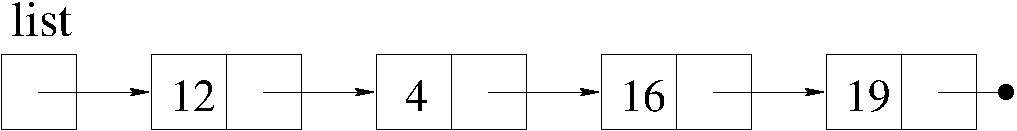
\includegraphics[width=4.5in]{linked_list_named.pdf}
\end{figure}

This list has no obvious order to the data values in the nodes.
It is either unordered or possibly ordered by time of insertion.
It is very easy to insert a new node at the start of a list, so
the list could be in decreasing time of insertion order.

The list is referenced using the pointer stored at the memory location
labelled {\tt list}.
The nodes on the list are not identified with specific labels in 
the code which maintains and uses the list.
The only way to access these nodes is by using the pointers
in the list.
\subsection{List node structure}

Our list node will have 2 fields: a data value and a pointer to the next
node.
The {\tt yasm} structure definition is
\begin{verbatim}
        struc   node
n_value resq    1
n_next  resq    1
        align   8
        endstruc
\end{verbatim}

The alignment instruction is not needed with 2 quad-words in the structure, but it may protect us from confusion later.

\subsection{Creating an empty list}

The first decision in designing a container structure is how to represent
an empty container.
In this linked list design we will take the simplest choice of using
a NULL pointer as an empty list.
Despite this simplicity it may be advantageous to 
have a function to create an empty list.

\begin{verbatim}
newlist:
        xor     eax, eax
        ret
\end{verbatim}

\subsection{Inserting a number into a list}

The decision to implement an empty list as a NULL pointer leaves a
small issue for insertion.
Each insertion will be at the start of the list which means that there
will be a new pointer stored in the list start pointer for each
insertion.
There are 2 possible ways to cope with this.
One way is to pass the address of the pointer into the insertion
function.
A second way is to have the insertion pointer return the new pointer
and leave it to the insertion code to assign the new pointer upon
return.
It is less confusing to dodge the address of a pointer problem.
Here is the insertion code:

\begin{verbatim}
;       list = insert ( list, k );
insert:
.list   equ     0
.k      equ     8
        push    rbp
        mov     rbp, rsp
        sub     rsp, 16
        mov     [rsp+.list], rdi  ; save list pointer
        mov     [rsp+.k], rsi     ; and k on stack
        mov     edi, node_size
        call    malloc            ; rax will be node pointer
        mov     r8, [rsp+.list]   ; get list pointer
        mov     [rax+n_next], r8  ; save pointer in node
        mov     r9, [rsp+.k]      ; get k
        mov     [rax+n_value], r9 ; save k in node
        leave
        ret
\end{verbatim}

\subsection{Traversing the list}

Traversing the list requires using an instruction like
\begin{verbatim}
        mov     rbx, [rbx+n_next]
\end{verbatim}
to advance from a pointer to one node to a pointer to the next node.
We start by inspecting the pointer to see if it is NULL.
If it is not then we enter the loop.
After processing a node we advance the pointer and repeat the loop
if the pointer is not NULL.
The {\tt print} function below traverses the list and prints each
data item.
The code shows a good reason why it is nice to have a few registers
protected in calls.
We depend on {\tt rbx} being preserved by {\tt printf}.

\begin{verbatim}
print:
        segment .data
.print_fmt:
        db      "%ld ",0
.newline
        db      0x0a,0
        segment .text
.rbx    equ     0
        push    rbp
        mov     rbp, rsp
        sub     rsp, 16           ; subtract multiples of 16
        mov     [rsp+.rbx], rbx   ; save old value of rbx
        cmp     rdi, 0
        je      .done
        mov     rbx, rdi
.more   lea     rdi, [.print_fmt]
        mov     rsi, [rbx+n_value]
        xor     eax, eax
        call    printf
        mov     rbx, [rbx+n_next]
        cmp     rbx, 0
        jne     .more
.done   lea     rdi, [.newline]
        xor     eax, eax
        call    printf
        mov     rbx, [rsp+.rbx]   ; restore rbx
        leave
        ret
\end{verbatim}

Last we have a {\tt main} function which creates a list, reads values using {\tt scanf}, inserts the values into the list
and prints the list after each insertion.
\begin{verbatim}
main:
.list   equ     0
.k      equ     8
        segment .data
.scanf_fmt:
        db      "%ld",0
        segment .text
        push    rbp
        mov     rbp, rsp
        sub     rsp, 16
        call    newlist
        mov     [rsp+.list], rax
.more   lea     rdi, [.scanf_fmt]
        lea     rsi, [rsp+.k]
        xor     eax, eax
        call    scanf
        cmp     rax, 1
        jne     .done
        mov     rdi, [rsp+.list]
        mov     rsi, [rsp+.k]
        call    insert
        mov     [rsp+.list], rax
        mov     rdi, rax
        call    print
        jmp     .more
.done   leave
        ret
\end{verbatim}

Here is a sample session using the program, entering the numbers 1 through 5:

\begin{verbatim}
1
1 
2
2 1 
3
3 2 1 
4
4 3 2 1 
5
5 4 3 2 1 
\end{verbatim}

You can see the the most recently printed number is at the first of the list.
By adding a function to get and remove (pop) the first element of the list, we could turn this
into a stack.
This is one of the exercises for this chapter.


\section{Doubly-linked lists}

A doubly-linked list has 2 pointers for each node: one points to the next node and one points to the previous node.
It becomes quite simple to manage a doubly-linked list if you make the list circular and if you retain an unused
cell at the start of the list.
Here is an example list with 4 data nodes:

\begin{figure}[h!]
\centering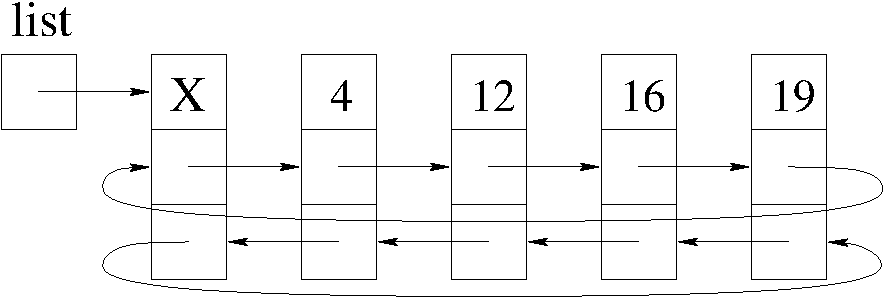
\includegraphics[width=4.5in]{doubly_linked_list.pdf}
\end{figure}

We see that the variable {\tt list} points to the first node of the list, called the ``head node''.
The head node has a value, but we never use the value.
The top pointer in each node points to the next node in the list and the bottom pointer points to the previous node
in the list.
The previous pointer of the head node is the last node in the list.
This makes this list capable of implementing a stack (last-in first-out), a queue (first-in first-out) or a double-ended queue
(deque).
The primary advantage of this design is that the list is never really empty - it can be logically empty but the head node
remains.
Furthermore, once a list is created, the pointer to the head node never changes.

\subsection{Doubly-linked list node structure}

Our list node will have 3 fields: a data value, a pointer to the next node and
a pointer to the previous node.
The {\tt yasm} structure definition is
\begin{verbatim}
        struc   node
n_value resq    1
n_next  resq    1
n_prev  resq    1
        align   8
        endstruc
\end{verbatim}

\subsection{Creating a new list}

The code for creating a new doubly-linked list allocates a new node and sets its next and previous pointers to
itself.
The calling function receives a pointer which does not change during the execution of the program.
Here is the creation code:
\begin{verbatim}
;       list = newlist();
newlist:
        push    rbp
        mov     rbp, rsp
        mov     edi, node_size
        call    malloc
        mov     [rax+n_next], rax
        mov     [rax+n_prev], rax
        leave
        ret
\end{verbatim}

When it returns the empty list looks like the diagram below:

\begin{center}
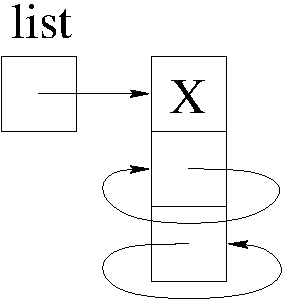
\includegraphics[width=1.0in]{empty_doubly_linked_list.pdf}
\end{center}

\subsection{Inserting at the front of the list}

To insert a new node at the front of the list you need to place the
head node's next pointer in the new node's next slot and place the
previous pointer from head's next into the new node's previous slot.
After doing that you can make the head node point forward to the new
node and make the head's former next point backwards to the new node.
There are illustrated in the diagram below.
The old links are in dashed lines and the new links are numbered,
with bold lines.

\begin{figure}[h!]
\centering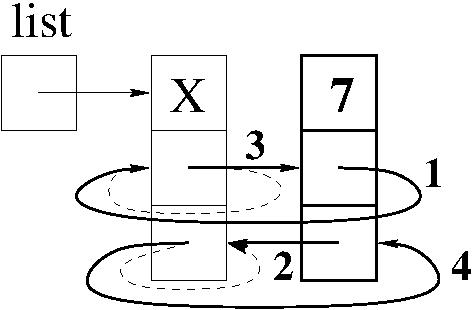
\includegraphics[width=1.5in]{insert_doubly_linked_list.pdf}
\end{figure}

One of the elegant features of the doubly-linked circular list is
the elimination of special cases.
Inserting the first node is done with exactly the same code as
inserting any other node.

The code for insertion is
\begin{verbatim}
;       insert ( list, k );
insert:
.list   equ     0
.k      equ     8
        push    rbp
        mov     rbp, rsp
        sub     rsp, 16
        mov     [rsp+.list], rdi  ; save list pointer
        mov     [rsp+.k], rsi     ; and k on stack
        mov     edi, node_size
        call    malloc            ; rax will be node pointer
        mov     r8, [rsp+.list]   ; get list pointer
        mov     r9, [r8+n_next]   ; get head's next
        mov     [rax+n_next], r9  ; set new node's next
        mov     [rax+n_prev], r8  ; set new node's prev
        mov     [r8+n_next], rax  ; set head's next
        mov     [r9+n_prev], rax  ; set new node's next's prev
        mov     r9, [rsp+.k]      ; get k
        mov     [rax+n_value], r9 ; save k in node
        leave
        ret
\end{verbatim}

\subsection{List traversal}

List traversal of a doubly-linked list is somewhat similar to
traversal of a singly-linked list.
We do need to skip past the head node and we need to test the
current pointer against the pointer to the head node to detect the
end of the list.
Here is the code for printing the list:
\begin{verbatim}
;       print ( list );
print:
        segment .data
.print_fmt:
        db      "%ld ",0
.newline:
        db      0x0a,0
        segment .text
.list   equ     0
.rbx    equ     8
        push    rbp
        mov     rbp, rsp
        sub     rsp, 16
        mov     [rsp+.rbx], rbx
        mov     [rsp+.list], rdi
        mov     rbx, [rdi+n_next]
        cmp     rbx, [rsp+.list]
        je      .done
.more   lea     rdi, [.print_fmt]
        mov     rsi, [rbx+n_value]
        call    printf
        mov     rbx, [rbx+n_next]
        cmp     rbx, [rsp+.list]
        jne     .more
.done   lea     rdi, [.newline]
        call    printf
        mov     rbx, [rsp+.rbx]
        leave
        ret
\end{verbatim}

\section{Hash tables}

A hash table is an efficient way to implement a dictionary.
The basic idea is that you compute a hash value for the key for each
item in the dictionary.
The purpose of the hash value is to spread the keys throughout an array.
A perfect hash function would map each key to a unique location in
the array used for hashing, but this is difficult to achieve.
Instead we must cope with keys which ``collide''.

The simplest way to cope with collisions is to use a linked list for
each location in the hash array.
Consider the illustration below:

\begin{figure}[h!]
\centering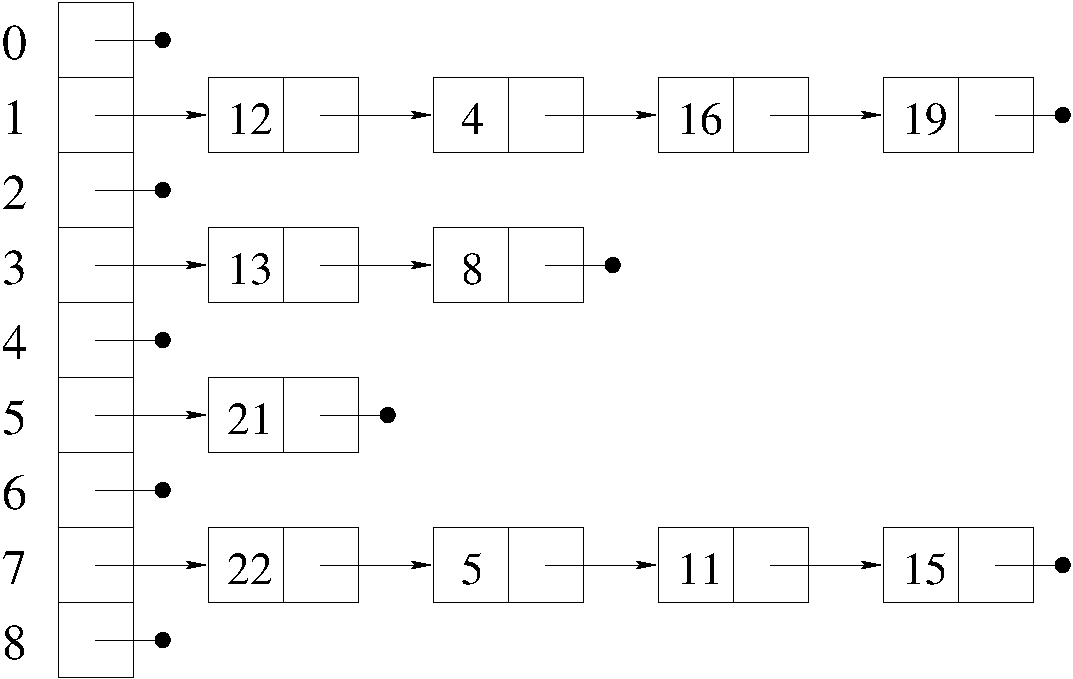
\includegraphics[width=0.6\textwidth]{hash_table.pdf}
\end{figure}

In this hash table, keys 12, 4, 16 and 9 all have hash values of 1 and
are placed on the list in location 1 of the hash array.
Keys 13 and 8 both have hash values 3 and are placed on the list in
location 3 of the array.
The remaining keys are mapped to 5 and 7.

One of the critical issues with hashing is to develop a good hashing
function.
A hashing function should appear almost random.
It must compute the same value for a particular key each time it is
called for the key, but the hash values aren't really important - it's the distribution of keys onto lists which matters.
We want a lot of short lists.
This means that the array size should be at least as large as the number
of keys expected.
Then, with a good hash function, the chains will generally be quite short.

\subsection{A good hash function for integers}

It is generally recommended that a hash table size be a prime number.
However this is not very important if there is no underlying pattern
to the numbers used as keys.
In that case you can simply use $n \mod t$ where $n$ is the key and
$t$ is the array size.
If there is a pattern like many multiples of the same number, then
using a prime number for $t$ makes sense.

Here is the hash function for the example code:
\begin{verbatim}
;       i = hash ( n );
hash    mov     rax, rdi
        and     rax, 0xff
        ret
\end{verbatim}
The table size is 256 in the example, so using {\tt and} gives $n \mod 256$.


\subsection{A good hash function for strings}

A good hash function for strings is to treat the string as containing polynomial coefficients and evaluate $p(n)$ for some prime number $n$.
In the code below we use the prime number 191 in the evaluation.
After evaluating the polynomial value, you can perform a modulus operation using the table size (100000 in the sample code).
\begin{verbatim}
    int hash ( unsigned char *s )
    {
        unsigned long h = 0;
        int i = 0;
        
        while ( s[i] ) {
            h = h*191 + s[i];
            i++;
        }
        return h % 100000;
    }
\end{verbatim}

\subsection{Hash table node structure and array}

In the sample hash table the table size is 256, so we need an array
of 256 NULL pointers when the program starts.
Since this is quite small, it is implemented in the data segment.
For a more realistic program, we would need a hash table creation
function to allocate an array and fill it with 0's.
Below is the declaration of the array and the structure definition
for the linked lists at each array location.

\begin{verbatim}
        segment .data
table   times 256 dq    0
        struc  node
n_value resq    1
n_next  resq    1
        align   8
        endstruc
\end{verbatim}

\subsection{Function to find a value in the hash table}

The basic purpose of a hash table is to store some data associated
with a key.
In the sample hash table we are simply storing the key.
The {\tt find} function below searches through the hash table looking
for a key.
If it is found, the function returns a pointer to the node with
the key.
If it is not found, it returns 0.
A more realistic program would probably return a pointer to the data
associated with the key.

The {\tt find} function operates by calling {\tt hash} to compute the
index in the hash array for the linked list which might hold the key being sought.
Then the function loops through the nodes on the list looking for the
key.

\begin{verbatim}
;       p = find ( n );
;       p = 0 if not found
find:
.n      equ     0
        push    rbp
        mov     rbp, rsp
        sub     rsp, 16
        mov     [rsp+.n], rdi
        call    hash
        mov     rax, [table+rax*8]
        mov     rdi, [rsp+.n]
        cmp     rax, 0
        je      .done
.more   cmp     rdi, [rax+n_value]
        je      .done
        mov     rax, [rax+n_next]
        cmp     rax, 0
        jne     .more
.done   leave
        ret
\end{verbatim}

\subsection{Insertion code}

The code to insert a key into the hash table begins by calling
{\tt find} to avoid inserting the key more than once.
If the key is found it skips the insertion code.
If the key is not found, the function calls {\tt hash} to determine
the index for the linked list to add the key to.
It allocates memory for a new node and inserts it at the start of the
list.

\begin{verbatim}
;       insert ( n );
insert:
.n      equ     0
.h      equ     8
        push    rbp
        mov     rbp, rsp
        sub     rsp, 16
        mov     [rsp+.n], rdi
        call    find
        cmp     rax, 0
        jne     .found
        mov     rdi, [rsp+.n]
        call    hash
        mov     [rsp+.h], rax
        mov     rdi, node_size
        call    malloc
        mov     r9, [rsp+.h]
        mov     r8, [table+r9*8]
        mov     [rax+n_next], r8
        mov     r8, [rsp+.n]
        mov     [rax+n_value], r8
        mov     [table+r9*8], rax
.found  leave
        ret
\end{verbatim}

\subsection{Printing the hash table}

The {\tt print} function iterates through the indices from 0 through 255,
printing the index number and the keys on each non-empty list.
It uses registers {\tt r12} and {\tt r13} for
safe storage of a loop counter to iterate through the locations of the
hash table array and for a pointer to loop through the nodes on each linked list.
This is more convenient than using registers which would require
saving and restoring around each {\tt printf} call.
It does require pushing and popping these 2 registers at the start and
end of the function to preserve them for calling functions.
Note that pushing and popping 16 bytes is necessary to preserve the
proper stack alignment.

You will notice that the code switches back and forth between the data and text segments so that {\tt printf} format strings will be placed
close to their point of use in the code.

\begin{verbatim}
print:
        push    rbp
        mov     rbp, rsp
        push    r12         ; i: integer counter for table
        push    r13         ; p: pointer for list at table[i]
        xor     r12, r12
.more_table:
        mov     r13, [table+r12*8]
        cmp     r13, 0
        je      .empty
        segment .data
.print1 db      "list %3d: ",0
        segment .text
        lea     rdi, [.print1]
        mov     rsi, r12
        call    printf
.more_list:
        segment .data
.print2 db      "%ld ",0
        segment .text
        lea     rdi, [.print2]
        mov     rsi, [r13+n_value]
        call    printf
        mov     r13, [r13+n_next]
        cmp     r13, 0
        jne     .more_list
        segment .data
.print3 db      0x0a,0
        segment .text
        lea     rdi, [.print3]
        call    printf
.empty  inc     r12
        cmp     r12, 256
        jl      .more_table
        pop     r13
        pop     r12
        leave
        ret
\end{verbatim}


\subsection{Testing the hash table}

The {\tt main} function for the hash table reads numbers with
{\tt scanf}, inserts them into the hash table and prints the hash
table contents after each insertion:
\begin{verbatim}
main:
.k      equ     0
        segment .data
.scanf_fmt:
        db      "%ld",0
        segment .text
        push    rbp
        mov     rbp, rsp
        sub     rsp, 16
.more   lea     rdi, [.scanf_fmt]
        lea     rsi, [rsp+.k]
        call    scanf
        cmp     rax, 1
        jne     .done
        mov     rdi, [rsp+.k]
        call    insert
        call    print
        jmp     .more
.done   leave
        ret
\end{verbatim}

Below is the printing of the hash table contents after
inserting 1, 2, 3, 4, 5, 256, 257, 258, 260, 513, 1025 and 1028.

\begin{verbatim}
list   0: 256 
list   1: 1025 513 257 1 
list   2: 258 2 
list   3: 3 
list   4: 1028 260 4 
list   5: 5 
\end{verbatim}


\section{Binary trees}

A binary tree is a structure with possible many nodes.
There is a single root node which can have left or right child nodes (or both).
Each node in the tree can have left or right child nodes (or both).

Generally binary trees are built with an ordering applied to keys in the nodes.
For example you could have a binary tree where every node divides keys into those less than the node's key
(in the left sub-tree) and those greater than the node's key (in the right sub-tree).
Having an ordered binary tree, often called a binary search tree, makes it possible to do fast searches
for a key while maintaining the ability to traverse the nodes in increasing or decreasing order.

Here we will present a binary tree with integer keys with the ordering being lower keys on the left and
greater keys on the right.
First are the structures used for the tree.

\subsection{Binary tree node and tree structures}

The nodes in the binary tree have an integer value and two pointers.
The structure definition below uses a prefix convention in naming the value field as {\tt n\_value} and
the left and right pointers as {\tt n\_left} and {\tt n\_right}.

\begin{verbatim}
        struc   node
n_value resq    1
n_left  resq    1
n_right resq    1
        align   8
        endstruc
\end{verbatim}

It would be possible to simply use a pointer to the root node to represent the tree.
However we could add features to the tree, like node deletion or balancing, which could change the root of
the tree.
It seems logical to store the root in a structure insulating us from future root changes in a tree.
We have also included in the tree structure a count of the number of nodes in the tree.

\begin{verbatim}
        struc   tree
t_count resq    1
t_root  resq    1
        align   8
        endstruc
\end{verbatim}

\subsection{Creating an empty tree}

The {\tt new\_tree} function allocates memory for a {\tt tree} structure and sets the count and the root
of the new tree to 0.
By having the root of the tree in a structure the code using the binary tree always refers to a particular
tree using the pointer returned by {\tt new\_tree}.

\begin{verbatim}
new_tree:
        push    rbp
        mov     rbp, rsp
        mov     rdi, tree_size
        call    malloc
        xor     edi, edi
        mov     [rax+t_root], rdi
        mov     [rax+t_count], rdi
        leave
        ret
\end{verbatim}

\subsection{Finding a key in a tree}

To find a key in a binary search tree you start with a pointer to the root node and compare the node's key with the key being sought.
If it's a match you're done.
If the target key is less than the node's key you change your pointer to the node's left child.
If the target key is greater than the node's key you change the pointer to the node's right child.
You then repeat these comparisons with the new node.
If you ever reach a NULL pointer, the key is not in the tree.
Below is the code for finding a key in a binary tree.
It returns a pointer to the correct tree node or NULL if not found.

\begin{verbatim}
;       p = find ( t, n );
;       p = 0 if not found
find:
        push    rbp
        mov     rbp, rsp
        mov     rdi, [rdi+t_root]
        xor     eax, eax
.more   cmp     rdi, 0
        je      .done
        cmp     rsi, [rdi+n_value]
        jl      .goleft
        jg      .goright
        mov     rax, rsi
        jmp     .done
.goleft:
        mov     rdi, [rdi+n_left]
        jmp     .more
.goright:
        mov     rdi, [rdi+n_right]
        jmp     .more
.done   leave
        ret
\end{verbatim}

\subsection{Inserting a key into the tree}

The first step in inserting a key is to use the {\tt find} function to see if the key is already there.
If it is, then there is no insertion.
If not, then a new tree node is allocated, its value is set to the new key value and its left and right child
pointers are set to NULL
Then it's time to find where to place this in the tree.

There is a special case for inserting the first node in the tree.
If the count of nodes in the tree is 0, then the count is incremented and the tree's root pointer is set to the new node.

If the tree is non-empty then you start by setting a current pointer to point to the root node.
If the new key is less than the current node's key, then the new node belongs in the left sub-tree.
To handle this you inspect the left child pointer of the current node.
If it is null, you have found the insertion point, so set the left pointer to the pointer of the new node.
Otherwise update your current node pointer to be the left pointer and start comparisons with this node.
If the key is not less than the current node's key, it must be greater than.
In that case you inspect the current node's right child pointer and either set it the new node's pointer or
advance your current pointer to the right child and repeat the comparison process.

\begin{verbatim}
;       insert ( t, n );
insert:
.n      equ     0
.t      equ     8
        push    rbp
        mov     rbp, rsp
        sub     rsp, 16
        mov     [rsp+.t], rdi
        mov     [rsp+.n], rsi
        call    find
        cmp     rax, 0
        jne     .done 
        mov     rdi, node_size
        call    malloc
        mov     rsi, [rsp+.n]
        mov     [rax+n_value], rsi
        xor     edi, edi
        mov     [rax+n_left], rdi
        mov     [rax+n_right], rdi
        mov     rdx, [rsp+.t]
        mov     rdi, [rdx+t_count]
        cmp     rdi, 0
        jne     .findparent
        inc     qword [rdx+t_count]
        mov     [rdx+t_root], rax
        jmp     .done
.findparent:
        mov     rdx, [rdx+t_root]
.repeatfind:
        cmp     rsi, [rdx+n_value]
        jl      .goleft
        mov     r8, rdx
        mov     rdx, [r8+n_right]
        cmp     rdx, 0
        jne     .repeatfind
        mov     [r8+n_right], rax
        jmp     .done
.goleft:
        mov     r8, rdx
        mov     rdx, [r8+n_left]
        cmp     rdx, 0
        jne     .repeatfind
        mov     [r8+n_left], rax
.done   leave
        ret
\end{verbatim}

\subsection{Printing the keys in order}

Printing the keys of a binary tree in order is easily performed by using recursion.
The basic idea is to print the keys in the left sub-tree, print the key of the root node and print the keys of
the right sub-tree.
The use of a special tree structure means that there needs to be a different
function to recursively print sub-trees
starting with the pointer to the root.
The main print function is named {\tt print} and the recursive function is called {\tt rec\_print}.

\begin{verbatim}
rec_print:
.t      equ     0
        push    rbp
        mov     rbp, rsp
        sub     rsp, 16
        cmp     rdi, 0
        je      .done
        mov     [rsp+.t], rdi
        mov     rdi, [rdi+n_left]
        call    rec_print
        mov     rdi, [rsp+.t]
        mov     rsi, [rdi+n_value]
        segment .data
.print  db      "%ld ",0
        segment .text
        lea     rdi, [.print]
        call    printf
        mov     rdi, [rsp+.t]
        mov     rdi, [rdi+n_right]
        call    rec_print
.done   leave
        ret

;       print(t);
print:
        push    rbp
        mov     rbp, rsp
        mov     rdi, [rdi+t_root]
        call    rec_print
        segment .data
.print  db      0x0a, 0
        segment .text
        lea     rdi, [.print]
        call    printf
        leave
        ret
\end{verbatim}

\vfill
\break
{\bf\large Exercises}

\begin{enumerate}
    \item Modify the singly-linked list code to implement a stack of strings.
    You can use the C {\tt strdup} function to make duplicates of strings that
    you insert.
    Write a main routine which creates a stack and enters a loop reading strings.
    If the string entered equals ``pop'', then pop the top of the stack and print that
    value.
    If the string entered equals ``print'', then print the contents of the stack.
    Otherwise push the string onto the stack.
    You code should exit when either {\tt scanf} or {\tt fgets} fails to read a string.
    
    \item Modify the doubly-linked list code to implement a queue of strings.
    Your main routine should read strings until no more are available.
     If the string entered equals ``dequeue'', then dequeue the oldest string from the queue and print it.
     If the string entered equals ``print'', then print the contents of the queue.
    Otherwise add the string onto the end of the queue.
    You code should exit when either {\tt scanf} or {\tt fgets} fails to read a string.
    
    \item Modify the hash table code to implement a hash table where you store strings
    and integers.
    The string will be the key and the integer will be its associated value.
    Your main routine should read lines using {\tt fgets} and read the text again using
    {\tt sscanf} to get a string and a number.
    If there is no number ({\tt sscanf} returns 1), then look for the string in the hash table and
    print its value if it there or else print an error message.
    If there is a string and a number ({\tt sscanf} returns 2), then add the string or update the string's
    value in the hash table.
    Your code should exit when {\tt fgets} fails to read a string.
    
    \item Implement a binary tree of strings and use it to read a file of text using {\tt fgets} and then
    print the lines of text in alphabetical order.
    
\end{enumerate}

\chapter{High performance assembly programming}

In this chapter we discuss some strategies for writing efficient x86-64 assembly language.
The gold standard is the efficiency of implementations written in C or C++ and compiled with
a good optimizing compiler.
The author uses gcc which produces executable code which is hard to beat.
Beating the compiler requires understanding your problem very well and knowing the instruction set
very well.
Furthermore you will need to use some strategy or feature which is not used by the compiler.

\section{General optimization strategies}

There are quite a few possible strategies for achieving high performance.
Many of these strategies are aggressively applied by modern compiler.
Some of these strategies can be profitably used in high level languages.
Here is a list of possible strategies:
\begin{itemize}
\item use a better algorithm
\item use C or C++
\item make efficient use of cache
\item common subexpression elimination
\item strength reduction
\item use registers efficiently
\item use fewer branches
\item convert loops to branch at the bottom
\item unroll loops
\item merge loops
\item split loops
\item interchange loops
\item move loop invariant code outside loops
\item remove recursion
\item eliminate stack frames
\item inline functions
\item eliminate dependencies to allow super-scalar execution
\item use specialized instructions
\end{itemize}

\section{Use a better algorithm}

The most important optimization strategy is to use a better algorithm.
It would be pointless to spend many hours tuning shell sort, when you could use the {\tt qsort} function within minutes and
achieve better performance.
Even better still would be to write C++ code and use the STL {\tt sort} function.
If you want to program efficiently you must become an expert in data structures and algorithms.

If you want to implement a dictionary you need to consider using a hash table.
A hash table of reasonable size has $O(1)$ expected time for finding a key.
A red-black tree has guaranteed $O(\lg n)$ expected lookup time.
However if you need to have ordered access to the keys in addition to simply
finding keys, then a red-black tree is a good choice.

Tuning code in assembly language will not convert an $O(n^2)$ algorithm into
an $O(n \lg n)$ algorithm.
Tuning can make things faster by some constant factor.
Only a better algorithm can reduce the complexity.

\section{Use C or C++}

This suggestion may seem a little crazy, but you can use a compiler for a variety of purposes.
First there is probably a large part of your application which is not worth optimizing and you could write
that code in C or C++ and save time, while achieving possibly the same performance.
Generally a small percentage of your code will consume a large percentage of
the time.
You might need to use a profiler to help locate the time-consuming parts.
It doesn't matter much if you have a process consuming several hours of CPU time
for you to tune a part of the program which consumes 10 seconds.

Second you should write a C version of your code and compare your code versus C to learn whether you have
done better than the compiler.
If you can't beat the compiler, then why use assembly language?
Your goal in using assembly is to make things run faster.
The goal should not be to write assembly code to prove that you can do it.

Finally you can use the {\tt -S} option of gcc to have it produce an assembly language file.
Studying this generated code may give you some ideas about how to write efficient assembly code.

\section{Efficient use of cache}

One of the goals in high performance computing is to keep the processing units
of the CPU busy.
A modern CPU like the Intel Core i7 operates at a clock speed around 3 GHz while
its main memory maxes out at about 21 GB/sec.
If your application ran strictly from data and instructions in memory using no
cache, then there would be roughly 7 bytes available per cycle.
The CPU has 4 cores which need to share the 21 GB/sec, so we're down to about 2
bytes per cycle per core from memory.
Yet each of these cores can have instructions being processed in 3 processing sub-units and 2 memory processing sub-units.
Each CPU can retire 4 instructions per cycle.
The same is true for the upcoming AMD Bulldozer CPUs
It requires much more than 2 bytes per cycle to keep instructions flowing in
a modern CPU.
To keep these CPUs fed requires 3 levels of cache.

I performed a short test to illustrate the effect of main memory access versus
cache on a Core i7 CPU.
The test consisted of executing 10 billion exclusive or operations on quad-words
in memory.
In the plot below you can see that the time depends heavily on the array size.
With an array of size 8000 bytes, the time as 1.5 seconds.
The time steadily grows through the use of the 8 MB of cache.
When the size is 80 million bytes the cache is nearly useless and a maximum of
about 5.7 seconds is reached.

\begin{center}
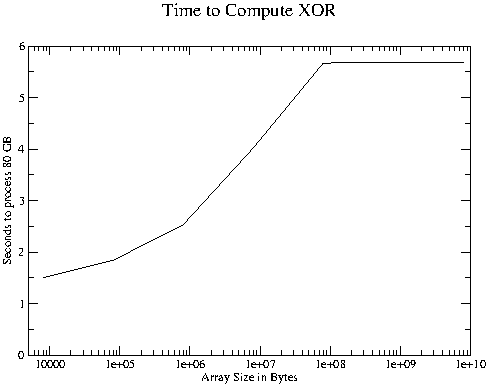
\includegraphics[width=0.7\textwidth]{xor.pdf}
\end{center}

A prime example of making efficient use of cache is in the implementation
of matrix multiplication.
Straight forward matrix multiplication in $O(n^3)$ where there are $n$ rows and
$n$ columns of data.
It is commonly coded as 3 nested loops.
However it can be broken up into blocks small enough for 3 blocks to fit in
cache for a nice performance boost.
Below are MFLOPS ratings for various block sizes for multiplying 2 1024x1024 
matrices in a C program.
There is considerable room for improvement by using assembly language to
take advantage of SSE or AVX instructions.

\begin{center}
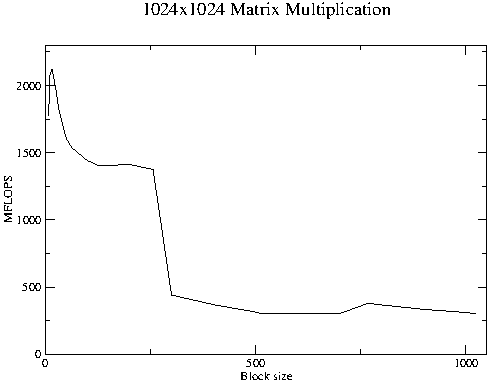
\includegraphics[width=0.7\textwidth]{mm.pdf}
\end{center}

\section{Common subexpression elimination}

Common subexpression is generally performed by optimizing compilers.
If you are to have any hope of beating the compiler, you must do the same thing.
Sometimes it may be hard to locate all common subexpressions.
This might be a good time to study the compiler's generated code to discover
what it found.
The compiler is tireless and efficient at its tasks.
Humans tend to overlook things.

\section{Strength reduction}

Strength reduction means using a simpler mathematical technique to get an
answer.
It is possible to computer $x^3$ using {\tt pow}, but it is probably faster
to compute {\tt x*x*x}.
If you need to compute $x^4$, then do it in stages
\begin{verbatim}
        x2 = x * x;
        x4 = x2 * x2;
\end{verbatim}
If you need to divide or multiply an integer by a power of 2, this can be done
more quickly by shifting.
If you need to divide more than one floating point number by $x$,
compute $1/x$ and multiply.


\section{Use registers efficiently}

Place commonly used values in registers.
It is nearly always better to place values in registers.
I once wrote a doubly nested loop in 32 bit mode where I had all my values in
registers.
{\tt gcc} generated faster code by using the stack for a few values.
These stack values probably remained in the level 1 cache and were almost as
good as being in registers.
Testing tells the truth.

\section{Use fewer branches}

Modern CPUs make branch predictions and will prepare the pipeline with
some instructions from one of the 2 possibilities when there is a conditional
branch.
The pipeline will stall when this prediction is wrong, so it will help
to try to make fewer branches.
Study the generated code from your compiler.
It will frequently reorder the assembly code to reduce the number of
branches.
You will learn some general techniques from the compiler.

\section{Convert loops to branch at the bottom}

If you code a while loop as written, there will be a conditional jump
at the top of the loop to branch past the loop and an unconditional jump at the bottom of the loop
to get back to the top.
It is always possible to transform the loop have a conditional branch at the
bottom.
You may need a one time use conditional jump before the top of the loop to handle
cases where the loop body should be skipped.

Here is a C {\tt for} loop converted to a {\tt do-while} loop.
First the {\tt for} loop:
\begin{verbatim}
        for ( i = 0; i < n; i++ ) {
            x[i] = a[i] + b[i];
        }
\end{verbatim}

Now the {\tt do-while} loop with an additional if:
\begin{verbatim}
        if ( n > 0 ) {
            i = 0;
            do {
                x[i] = a[i] + b[i];
                i++;
            } while ( i < n );
        }
\end{verbatim}

Please do not adopt this style of coding in C or C++.
The compiler will handle {\tt for} loops quite well.
In fact the simplicity of the {\tt for} loop might allow the compiler
to generate better code.
I presented this in C simply to get the point across more quickly.


\section{Unroll loops}

Unrolling loops is another technique used by compilers.
The primary advantage is that there will be fewer loop control instructions
and more instructions doing the work of the loop.
A second advantage is that the CPU will have more instructions available to fill
its pipeline with a longer loop body.
Finally if you manage to use registers with little or no dependencies between
the separate sections of unrolled code, then you open up the possibility for
a super-scalar CPU (most modern CPUs) to execute multiple original iterations
in parallel.
This is considerably easier with 16 registers than with 8.

Let's consider some code to add up all the numbers in an array of quad-words.
Here is the assembly code for the simplest version:
\begin{verbatim}
        segment .text
        global  add_array
add_array:
        xor     eax, eax
.add_words:
        add     rax, [rdi]
        add     rdi, 8
        dec     rsi
        jg      .add_words
        ret
\end{verbatim}

Here is a version with the loop unrolled 4 times:
\begin{verbatim}
        segment .text
        global  add_array
add_array:
        push    r15
        push    r14
        push    r13
        push    r12
        push    rbp
        push    rbx
        xor     eax, eax
        mov     rbx, rax
        mov     rcx, rax
        mov     rdx, rax
.add_words:
        add     rax, [rdi]
        add     rbx, [rdi+8]
        add     rcx, [rdi+16]
        add     rdx, [rdi+16]
        add     rdi, 32
        sub     rsi, 4
        jg      .add_words
        add     rcx, rdx
        add     rax, rbx
        add     rax, rcx
        pop     rbx
        pop     rbp
        pop     r12
        pop     r13
        pop     r14
        pop     r15
        ret
\end{verbatim}

There may have been some way to use fewer callee-save registers, but the
choices I made simplified the coding.
In the unrolled code I am accumulating partial sums in {\tt rax}, {\tt rbx},
{\tt rcx} and {\tt rdx}.
These partial sums are combined after the loop.
Executing a test program with 1000000 calls to add up an array of 10000 quad-words took 3.9 seconds for the simple version and 2.44 seconds for the unrolled
version.
There is so little work to do per data element that the 2 programs start becoming
memory bandwidth limited with large arrays, so I tested a size which fit easily in cache.

\section{Merge loops}

If you have 2 {\tt for} loops iterating over the same sequence of values and
there is no dependence between the loops, it seems like a no-brainer to merge
the loops.
Consider the following 2 loops:
\begin{verbatim}
        for ( i = 0; i < 1000; i++ ) a[i] = b[i] + c[i];
        for ( j = 0; j < 1000; j++ ) d[j] = b[j] - c[j];
\end{verbatim}
This can easily be merged to get:
\begin{verbatim}
        for ( i = 0; i < 1000; i++ ) {
            a[i] = b[i] + c[i];
            d[i] = b[i] - c[i];
        }
\end{verbatim}

In general merging loops can increase the size of a loop body, decreasing
the overhead percentage and helping to keep the pipeline full.
In this case there is additional gain from loading the values of {\t b} and
{\tt c} once rather than twice.

\section{Split loops}

We just got through discussing how merging loops was a good idea.
Now we are going to learn the opposite - well for some loops.
If a loop is operating on 2 independent sets of data, then it could be
split into 2 loops.
This can improve performance if the combined loop is exceeding the cache
capacity.
There is a trade-off between better cache usage and more instructions in the
pipeline.
Sometime merging is better and sometimes splitting is better.

\section{Interchange loops}

Suppose you wish to place 0's in a 2-dimensional array in C.  You have
2 choices:
\begin{verbatim}
        for ( i = 0; i < n; i++ ) {
            for ( j = 0; j < n; j++ ) {
                x[i][j] = 0;
            }
        }
\end{verbatim}
or
\begin{verbatim}
        for ( j = 0; j < n; j++ ) {
            for ( i = 0; i < n; i++ ) {
                x[i][j] = 0;
            }
        }
\end{verbatim}

Which is better?  In C the second index increments faster than the first.
This means that {\tt x[0][1]} is immediately after {\tt x[0][0]}.
On the other hand {\tt x[1][0]} is {\tt n} elements after {\tt x[0][0]}.
When the CPU fetches data into the cache it fetches more than a few bytes and
cache writes to memory behave similarly, so the first loop makes more sense.
If you have the extreme misfortune of having an array which is too large for
your RAM, then you may experience virtual memory thrashing with the second
version.
This could turn into a disk access for each array access.

\section{Move loop invariant code outside loops}

This might be a fairly obvious optimization to perform.
It's another case where studying the compiler's generated code might
point out some loop invariant code which you have overlooked.

\section{Remove recursion}

If it easy to eliminate recursion then it will nearly always improve efficiency.
Often it is easy to eliminate ``tail'' recursion where the last action of a function is a recursive call.
This can generally be done by branching to the top of the function.
On the other hand if you try to eliminate recursion for a function like quicksort
which makes 2 non-trivial recursive calls, you will be forced to ``simulate'' recursion using you own stack.
This may make things slower.
In any case the effect is small, since the time spent making recursive calls
in quicksort is small.

\section{Eliminate stack frames}

For leaf functions it is not necessary to use stack frames.
In fact if you have non-leaf functions which call your own functions and no
others then you can omit the frame pointers from these too.
The only real reason for frame pointers is for debugging.
There is a requirement for leaving the stack on 16 byte boundaries, but this
only becomes as issue with functions which have local variables (on the stack)
which participate in aligned 16 or 32 byte accesses which can either fail or
be slower.
If you know that your own code is not using those instructions, then neither
frame pointers nor frame alignment are important other than for debugging.

\section{Inline functions}

As part of optimization compilers can in-line small functions.
This reduces the overhead significantly.
If you wish to do this, you might be interested in exploring macros which
can make your code easier to read and write and operate much like a function
which has been in-lined.

\section{Eliminate dependencies to allow super-scalar execution}

Modern CPUs inspect the instruction stream looking ahead for instructions which
do not depend upon results of earlier instructions.
This is called ``out of order execution''.
If there is less dependency in your code, then the CPU will execute more
instructions out of order and your program will run more quickly.

As an example of this I modified the previous {\tt add\_array} function with
unrolled loops to accumulate all 4 values in the loop into {\tt rax}.
This increased the time from 2.44 seconds to 2.75 seconds.

\section{Use specialized instructions}

So far we have seen the conditional move instruction which is fairly
specialized and also the packed floating point instructions.
There are many specialized instructions in the x86-64 architecture which
are more difficult for a compiler to apply.
A human can reorganize an algorithm to add the elements of an array somewhat
like I did with loop unrolling except to keep 4 partial sums in one AVX
register.
Combining the 4 parts of the AVX register can be done after the loop.
This can make the adding even faster, since 4 adds can be done in one instruction.
This technique can also be combined with loop unrolling for additional
performance.
This will be explored in detail in the SSE and AVX chapters.

\vfill
\break
{\large Exercises}

\begin{enumerate}
    \item Given an array of 3D points defined in a structure with x, y and
    z components, write a function to compute a distance matrix with
    the distances between each pair of points.
    \item Given a 2D array, $M$, of floats of length of dimensions $n$ and 4, and
    a vector, $v$, of 4 floats compute $Mv$.
    
\end{enumerate}


\chapter{Counting bits in an array}

In this chapter we explore several solutions to the problem of counting
all the 1 bits in an array of quad-word integers.
For each test we use the same C main program and implement a different function
counting the number of 1 bits in the array.
All these functions implement the same prototype:
\begin{verbatim}
    long popcnt_array ( long *a, int size );
\end{verbatim}

\section{C function}

The first solution is a straightforward C solution:
\begin{verbatim}
    long popcnt_array ( long *a, int size )
    {
        int w, b;
        long word;
        long n;

        n = 0;
        for ( w = 0; w < size; w++ ) {
            word = a[w];
            n += word & 1;
            for ( b = 1; b < 64; b++ ) {
                n += (word >> b) & 1;
            }
        }
        return n;
    }
\end{verbatim}

The testing consists of calling the {\tt popcnt\_array} 1000 times
with an array of 100000 longs (800000 bytes).
Compiling with optimization level zero (option {\tt -O0}) the test took 14.63 seconds.
With optimization level 1, it took 5.29 seconds, with level 2 it took 5.29
seconds again, and with level 3 it took 5.37 seconds.
Finally adding {\tt -funroll-all-loops}, it took 4.74 seconds.

The algorithm can be improved by noticing that frequently the upper bits of
the quad-words being tested might be 0.
We can change the inner for loop into a while loop:
\begin{verbatim}
    long popcnt_array ( unsigned long *a, int size )
    {
        int w, b;
        unsigned long word;
        long n;
    
        n = 0;
        for ( w = 0; w < size; w++ ) {
            word = a[w];
            while ( word != 0 ) {
                n += word & 1;
                word >>= 1;
            }
        }
        return n;
    }
\end{verbatim}

Using the maximum optimization options the version takes 3.34 seconds.
This is an instance of using a better algorithm.

\section{Counting 1 bits in assembly}

It is not too hard to unroll the loop for working on 64 bits into
64 steps of working on 1 bit.
In the assembly code which follows one fourth of the bits of each word
are placed in {\tt rax}, one fourth in {\tt rbx}, one fourth in {\tt rcx}
and one fourth in {\tt rdx}.
Then each fourth of the bits are accumulated using different registers.
This allows considerable freedom for the computer to use out-or-order
execution with the loop.

\begin{verbatim}
        SECTION .text
        global  popcnt_array           ; let the linker know about popcnt_array

        ; integer and address parameters are in rdi, rsi, rdx, rcx, r8, r9
        ; floating point parameters are in xmm0-7
popcnt_array:
        push    rbx
        push    rbp
        push    r12
        push    r13
        push    r14
        push    r15
        xor     eax, eax
        xor     ebx, ebx
        xor     ecx, ecx
        xor     edx, edx
        xor     r12d, r12d
        xor     r13d, r13d
        xor     r14d, r14d
        xor     r15d, r15d
.count_words:
        mov     r8, [rdi]
        mov     r9, r8
        mov     r10, r8
        mov     r11, r9
        and     r8, 0xffff
        shr     r9, 16
        and     r9, 0xffff
        shr     r10, 32
        and     r10, 0xffff
        shr     r11, 48
        and     r11, 0xffff

        mov     r12w, r8w
        and     r12w, 1
        add     rax, r12
        mov     r13w, r9w
        and     r13w, 1
        add     rbx, r13
        mov     r14w, r10w
        and     r14w, 1
        add     rcx, r14
        mov     r15w, r11w
        and     r15w, 1
        add     rdx, r15

%rep 15
        shr     r8w, 1
        mov     r12w, r8w
        and     r12w, 1
        add     rax, r12
        shr     r9w, 1
        mov     r13w, r9w
        and     r13w, 1
        add     rbx, r13
        shr     r10w, 1
        mov     r14w, r10w
        and     r14w, 1
        add     rcx, r14
        shr     r11w, 1
        mov     r15w, r11w
        and     r15w, 1
        add     rdx, r15
%endrep
        add     rdi, 8
        dec     rsi
        jg      .count_words
        add     rax, rbx
        add     rax, rcx
        add     rax, rdx
        pop     r15
        pop     r14
        pop     r13
        pop     r12
        pop     rbp
        pop     rbx
        ret
\end{verbatim}

This is an unfortunate side effect - the use of a repeat section with repeats
15 times.  This makes for function of 1123 bytes.  Perhaps it was worth it
to execute the test in 2.52 seconds.  The object file is only 240 more bytes than
the C code with unrolled loops.

\section{Precomputing the number of bits in each byte}

The next algorithmic improvement comes from recognizing that we can precompute
the number of bits in each possible bit pattern and use an array of 256 bytes
to store the number of bits in each byte.
Then counting the number of bits in a quad-word consists of using the 8 bytes
of the quad-word as indices into the array of bit counts and adding them up.

Here is the C function for adding the number of bits in the array without
the initialization of the {\tt count} array:
\begin{verbatim}
    long popcnt_array ( long *a, int size )
    {
        int b;
        long n;
        int word;
    
        n = 0;
        for ( b = 0; b < size*8; b++ ) {
            word = ((unsigned char *)a)[b];
            n += count[word];
        }
        return n;
    }
\end{verbatim}

This code took 0.24 seconds for the test, so we have a new winner.
I tried hard to beat this algorithm using assembly language, but managed only a tie.

\section{Using the popcnt instruction}

A new instruction included in the Core i series processors in {\tt popcnt} which
gives the number of 1 bits in a 64 bit register.
So on the right computers, we can employ the technique of using a specialized 
instruction:

\begin{verbatim}
        segment .text
        global  popcnt_array
popcnt_array:
        xor     eax, eax
        xor     r8d, r8d
        xor     ecx, ecx
.count_more:
        popcnt  rdx, [rdi+rcx*8]
        add     rax, rdx
        popcnt  r9, [rdi+rcx*8+8]
        add     r8, r9
        add     rcx, 2
        cmp     rcx, rsi
        jl      .count_more
        add     rax, r8
        ret
\end{verbatim}

We have a new winner on the Core i7 at 0.04 seconds which is 10 times fast as
all the previous efforts could yield.

\vfill
\break
{\bf\large Exercises}

\begin{enumerate}
    \item Write a function to convert an array of ASCII characters into
    EBCDIC and another to convert back to ASCII.
    \item For 2 arrays of ASCII characters write a function to find the
    longest common substring.
\end{enumerate}


\chapter{Sobel filter}

The Sobel filter is an edge detection filter used in image processing.
The operation of the filter is to process 3x3 windows of data by convolving
each pixel by one 3x3 matrix to produce an edge measure in the $x$ direction
and another in the $x$ direction.
Here are the 2 matrices
$$
S_x = \left[\begin{matrix}
                -1 & 0 & 1 \\
                -2 & 0 & 2 \\
                -1 & 0 & 1
                \end{matrix}\right]
                \qquad\qquad
S_y = \left[\begin{matrix}
                -1 & -2 & -1 \\
                 0 & 0 & 0 \\
                 1 & 2 & 1
                \end{matrix}\right]
$$
For an individual pixel $I_{r,c}$ the $x$ edge measure, $G_x$, is computed
by
$$G_x = \sum_{i=-1}^{1}\sum_{j=-1}^1(S_{x,i,j}* I_{r+i,c+i})$$
where we have conveniently numbered the rows and columns of $S_x$ starting with
-1.  Similarly we compute $G_y$ using
$$G_y = \sum_{i=-1}^{1}\sum_{j=-1}^1(S_{y,i,j}*I_{r+i,c+i})$$
Next we show how to get the magnitude of the edge measure, $G$,
$$G = \sqrt{G_x^2+G_y^2}$$

\section{Sobel in C}

Here is a C function which computes the Sobel edge magnitude for an
image of arbitrary size:
\begin{verbatim}
#include <math.h>

#define matrix(a,b,c) a[(b)*(cols)+(c)]

void sobel ( unsigned char *data, float *output, long rows, long cols )
{
    int r, c;
    int gx, gy;


    for ( r = 1; r < rows-1; r++ ) {
        for ( c = 1; c < cols-1; c++ ) {
            gx = -matrix(data,r-1,c-1) + matrix(data,r-1,c+1) +
                 -2*matrix(data,r,c-1) + 2*matrix(data,r,c+1) +
                 -matrix(data,r+1,c-1) + matrix(data,r+1,c+1);
            gy = -matrix(data,r-1,c-1) - 2*matrix(data,r-1,c)
                 - matrix(data,r-1,c+1) +
                 matrix(data,r+1,c-1) + 2*matrix(data,r+1,c)
                 + matrix(data,r+1,c+1);
            matrix(output,r,c) = sqrt((float)(gx)*(float)(gx)+
                                      (float)(gy)*(float)(gy));
        }
    }
}
\end{verbatim}

This code was compiled with {-O3} optimization and full loop unrolling.
Testing with $1024\times1024$ images showed that it computed 161.5 Sobel
magnitude images per second.
Testing with 1000 different images to cut down on the effect of cached
images, this code produced 158 images per second.
Clearly the code is dominated by mathematics rather than memory bandwidth.

\section{Sobel computed using SSE instructions}

Sobel was chosen as a good example of an algorithm which manipulates
data of many types.
First the image data is byte data.
The {\tt movdqu} instruction was used to transfer 16 adjacent pixels 
from one row of image.
These pixels were processed to produce the contribution of their
central 14 pixels to $G_x$ and $G_y$.
The 16 pixels were transferred from the image one row down from the first
16 pixels.
These pixels were processed in the same way adding more the $G_x$ and $G_y$.
Finally 16 more pixels 2 rows down from the first 16 were transferred and
their contributions to $G_x$ and $G_y$ were computed.
Then these contributions were combined, squared, added together, converted
to 32 bit floating point and square roots were computed for the 13 output
pixels which were placed in the output array.

Tested on the same Core i7 computer, this code produced 1063 Sobel magnitude
images per second.
Testing with 1000 different images this code produced 980 images per second, which is about 6.2 times as fast as the C version.

Here are the new instructions used in this code:

\begin{description}
    \item [pxor] This instruction performs an exclusive or on a 128 XMM
          source register or memory and stores the result in the destination register.
    \item [movdqa] This instruction moves 128 bits of aligned data from memory
                   to a register, from a register to memory, or from a register
                   to a register.
    \item [movdqu] This instruction moves 128 bits of unaligned data from memory
                   to a register, from a register to memory, or from a register
                   to a register.
    \item [psrldq] This instruction shifts the destination XMM register right the
                   number of bytes specified in the second immediate operand.
    \item [punpcklbw] This instruction unpacks the low 8 bytes of 2 XMM registers
                   and intermingles them. I used this with the second register
                   holding all 0 bytes to form 8 words in the destination.
    \item [punpckhbw] This instruction unpacks the upper 8 bytes of 2 XMM
                   registers and intermingles them.
    \item [paddw]  This instruction adds 8 16 bit integers from the second
                   operand to the first operand.  At least one of the operands
                   must be an XMM register and one can be a memory field.
    \item [psubw]  This instruction subtracts the second set of 8 16 bit integers
                   from the first set.
    \item [pmullw] This instruction multiplies the first set of 8 16 bit integers
                   times the second set and store the low order 16 bits of the
                   products in the first operand.
    \item [punpcklwd]   This instruction unpacks and interleaves words from
                   the lower halves 2 XMM registers into the destination register.
    \item [punpckhwd]   This instruction unpacks and interleaves words from
                   the upper halves 2 XMM registers into the destination register.
    \item [cvtdq2ps]  This instruction converts 4 double word integers into
                   4 double word floating point values.
    
\end{description}

Here is the assembly code:

\begin{verbatim}
%macro  multipush 1-*       ; I needed to push and pop all callee save
    %rep  %0                ; registers, so I used macros from the
        push    %1          ; yasm documentation.
        %rotate 1
    %endrep
%endmacro

%macro  multipop 1-*
    %rep %0
        %rotate -1
        pop     %1
    %endrep
%endmacro

;       sobel ( input, output, rows, cols );
;       char input[rows][cols]
;       float output[rows][cols]
;       boundary of the output array will be unfilled
;
        segment .text
        global  sobel, main
sobel:
.cols   equ     0
.rows   equ     8
.output equ     16
.input  equ     24
.bpir   equ     32
.bpor   equ     40
        multipush   rbx, rbp, r12, r13, r14, r15
        sub     rsp, 48
        cmp     rdx, 3
        jl      .noworktodo
        cmp     rcx, 3
        jl      .noworktodo
        mov     [rsp+.input], rdi
        mov     [rsp+.output], rsi
        mov     [rsp+.rows], rdx
        mov     [rsp+.cols], rcx
        mov     [rsp+.bpir], rcx
        imul     rcx, 4
        mov     [rsp+.bpor], rcx

        mov     rax, [rsp+.rows]; count of rows to process
        mov     rdx, [rsp+.cols]
        sub     rax, 2
        mov     r8, [rsp+.input]
        add     r8, rdx
        mov     r9, r8          ; address of row
        mov     r10, r8
        sub     r8, rdx         ; address of first byte of row-1
        add     r10, rdx        ; address of first byte of row+1
        pxor    xmm13, xmm13
        pxor    xmm14, xmm14
        pxor    xmm15, xmm15
.more_rows:
        mov     rbx, 1          ; first column to process
.more_cols:
        movdqu  xmm0, [r8+rbx-1]    ; data for 1st row of 3
        movdqu  xmm1, xmm0
        movdqu  xmm2, xmm0
        pxor    xmm9, xmm9
        pxor    xmm10, xmm10
        pxor    xmm11, xmm11
        pxor    xmm12, xmm12
        psrldq  xmm1, 1             ; shift the pixels 1 to the right
        psrldq  xmm2, 2             ; shift the pixels 2 to the right
                                    ; Now the lowest 14 values of
                                    ; xmm0, xmm1 and xmm2 are lined
                                    ; up properly for applying the
                                    ; top row of the 2 matrices.
        movdqa  xmm3, xmm0
        movdqa  xmm4, xmm1
        movdqa  xmm5, xmm2
        punpcklbw   xmm3, xmm13     ; The low 8 values are now words 
        punpcklbw   xmm4, xmm14     ; in registers xmm3, xmm4, and
        punpcklbw   xmm5, xmm15     ; and xmm5 - ready for arithmetic.
        psubw   xmm11, xmm3         ; xmm11 will hold 8 values of Gx
        psubw   xmm9, xmm3          ; xmm9 will hold 8 values of Gy
        paddw   xmm11, xmm5         ; Gx subtracts left, adds right pixels
        psubw   xmm9, xmm4          ; Gy subtracts 2 times middle pixel
        psubw   xmm9, xmm4
        psubw    xmm9, xmm5         ; Final subtraction for Gy
        punpckhbw  xmm0, xmm13      ; Now convert top 8 bytes to words
        punpckhbw  xmm1, xmm14      
        punpckhbw  xmm2, xmm15
        psubw   xmm12, xmm0         ; Perform the same arithmetic
        psubw   xmm10, xmm0         ; storing these 6 values in
        paddw   xmm12, xmm2         ; xmm12 and xmm10
        psubw   xmm10, xmm1
        psubw   xmm10, xmm1
        psubw   xmm10, xmm2     
        
        movdqu  xmm0, [r9+rbx-1]    ; data for 2nd row of 3
        movdqu  xmm2, xmm0          ; repetition of math from 1st row
        psrldq  xmm2, 2             ; with nothing added to Gy registers
        movdqa  xmm3, xmm0
        movdqa  xmm5, xmm2
        punpcklbw   xmm3, xmm13
        punpcklbw   xmm5, xmm15         ; 8 values for 1st row
        psubw   xmm11, xmm3
        psubw   xmm11, xmm3
        paddw   xmm11, xmm5
        paddw   xmm11, xmm5
        punpckhbw  xmm0, xmm13
        punpckhbw  xmm2, xmm15
        psubw   xmm12, xmm0
        psubw   xmm12, xmm0
        paddw   xmm12, xmm2
        paddw   xmm12, xmm2     ; finished tally for 2nd row, last 6

        movdqu  xmm0, [r10+rbx-1]   ; data for 3rd row of 3
        movdqu  xmm1, xmm0
        movdqu  xmm2, xmm0
        psrldq  xmm1, 1
        psrldq  xmm2, 2
        movdqa  xmm3, xmm0
        movdqa  xmm4, xmm1
        movdqa  xmm5, xmm2
        punpcklbw   xmm3, xmm13
        punpcklbw   xmm4, xmm14
        punpcklbw   xmm5, xmm15     ; 8 values for 3rd row
        psubw   xmm11, xmm3
        paddw   xmm9, xmm3
        paddw   xmm11, xmm5
        paddw   xmm9, xmm4
        paddw   xmm9, xmm4
        paddw   xmm9, xmm5          ; finished tally for 3rd row, 1st 8
        punpckhbw  xmm0, xmm13
        punpckhbw  xmm1, xmm14
        punpckhbw  xmm2, xmm15
        psubw   xmm12, xmm0
        paddw   xmm10, xmm0
        paddw   xmm12, xmm2
        paddw   xmm10, xmm1
        paddw   xmm10, xmm1
        paddw   xmm10, xmm2     ; finished tally for 3rd row, last 6

        pmullw  xmm9, xmm9      ; square Gx and Gy values
        pmullw  xmm10, xmm10
        pmullw  xmm11, xmm11
        pmullw  xmm12, xmm12
        paddw   xmm9, xmm11     ; sum of squares
        paddw   xmm10, xmm12
        movdqa  xmm1, xmm9
        movdqa  xmm3, xmm10
        punpcklwd xmm9, xmm13   ; Convert low 4 words to double words
        punpckhwd xmm1, xmm13   ; Convert high 4 words to double words
        punpcklwd xmm10, xmm13  ; Convert low 4 words to double words
        punpckhwd xmm3, xmm13   ; Convert high 4 words to double words
        cvtdq2ps  xmm0, xmm9    ; Convert to floating point
        cvtdq2ps  xmm1, xmm1    ; Convert to floating point
        cvtdq2ps  xmm2, xmm10   ; Convert to floating point
        cvtdq2ps  xmm3, xmm3    ; Convert to floating point
        sqrtps    xmm0, xmm0    ; Take sqrt to get magnitude
        sqrtps    xmm1, xmm1    ; Take sqrt to get magnitude
        sqrtps    xmm2, xmm2    ; Take sqrt to get magnitude
        sqrtps    xmm3, xmm3    ; Take sqrt to get magnitude
        movups    [rsi+rbx*4], xmm0
        movups    [rsi+rbx*4+16], xmm1
        movups    [rsi+rbx*4+32], xmm2
        movlps    [rsi+rbx*4+48], xmm3

        add     rbx, 14         ; process 14 Sobel values
        cmp     rbx, rdx
        jl      .more_cols
        
        add     r8, rdx
        add     r9, rdx
        add     r10, rdx
        add     rsi, [rsp+.bpor]
        sub     rax, 1          ; 1 fewer row to process
        cmp     rax, 0
        jg      .more_rows
.noworktodo:
        add     rsp, 48
        multipop    rbx, rbp, r12, r13, r14, r15
        ret
\end{verbatim}

\vfill
\break
{\bf\large Exercises}

\begin{enumerate}
    \item Convert the sobel function into a function to perform an arbitrary
    convolution of an image with a $3\times 3$ matrix.
    \item Write an assembly function to convert an image into a run-length
    encoded image.
    \item Write a function to fill an array with pseudo-random numbers
    derived by using 4 separate interleaved sequences based on
    the formula
    $$X_{n+1} = (a X_n + c) \mod m$$
    Use $m=32$ for all 4 sequences.
    Use 1664525, 22695477, 1103515245 and 214013 for the values for $a$ and
    1013904223, 1, 12345 and 2531011 for the values for $c$.
    
\end{enumerate}

\chapter{Computing Correlation}

The final example of optimization is computing the correlation between two
variables $x$ and $y$ given $n$ sample values.
One way to compute correlation is using
$$r_{xy}= \frac{\sum_{i=1}^n (x_i - \bar{x})(y_i-\bar{y})}
{\sqrt{\sum_{i=1}^n(x_i-\bar{x})^2\sum_{i=1}^n(y_i-\bar{y})^2}} $$
But this formula requires two passes through the data - one pass to compute averages and a second pass to complete the formula.
There is a less intuitive formula which is more amenable to computation:
$$r_{xy} = \frac{n\sum x_iy_i - \sum x_i \sum y_i}
{\sqrt{n\sum x_i^2 - (\sum x_i)^2} \sqrt{n\sum y_i^2 - (\sum y_i)^2} }$$

The computational formula requires computing 5 sums when you scan the data:
the sum of $x_i$, the sum of $y_i$, the sum of $x_i^2$, the sum of $y_i^2$ and
the sum of $x_iy_i$.
After computing these 5 sums there is a small amount of time required for
implementing the computational formula.

\section{C implementation}


The C computation is performed in the {\tt corr} function
given below:

\begin{verbatim}
#include <math.h>
double corr ( double x[], double y[], long n )
{
    double sum_x, sum_y, sum_xx, sum_yy, sum_xy;
    long i;

    sum_x = sum_y = sum_xx = sum_yy = sum_xy = 0.0;
    for ( i = 0; i < n; i++ ) {
        sum_x += x[i];
        sum_y += y[i];
        sum_xx += x[i]*x[i];
        sum_yy += y[i]*y[i];
        sum_xy += x[i]*y[i];
    }
    return (n*sum_xy-sum_x*sum_y)/
           sqrt((n*sum_xx-sum_x*sum_x)*(n*sum_yy-sum_y*sum_y));
}
\end{verbatim}

The {\tt gcc} compiler generated assembly code which used all 16 of the XMM
registers as it unrolled the loop to process 4 iterations of the {\tt for}
loop in the main loop of the assembly version.
The compiler also correctly handled the extra data values when the array size
was not a multiple of four.
Performing 1 million call to compute correlation on 2 arrays of size 10000
required 13.44 seconds for the C version.
This is roughly 5.9 GFLOPs which is quite impressive for compiled code.

\section{Implementation using SSE instructions}

A version of the {\tt core} function 
was written using SSE instructions which will execute on many modern
computers.
Here is the SSE version:

\begin{verbatim}
        segment .text
        global corr

; rdi, rsi, rdx, rcx, r8, r9
;
;       rdi:  x array
;       rdi:  y array
;       rcx:  loop counter
;       rdx:  n
;       xmm0: 2 parts of sum_x
;       xmm1: 2 parts of sum_y
;       xmm2: 2 parts of sum_xx
;       xmm3: 2 parts of sum_yy
;       xmm4: 2 parts of sum_xy
;       xmm5: 2 x values - later squared
;       xmm6: 2 y values - later squared
;       xmm7: 2 xy values
corr:
        xor     r8, r8
        mov     rcx, rdx
        subpd   xmm0, xmm0
        movapd   xmm1, xmm0
        movapd   xmm2, xmm0
        movapd   xmm3, xmm0
        movapd   xmm4, xmm0
        movapd   xmm8, xmm0
        movapd   xmm9, xmm0
        movapd   xmm10, xmm0
        movapd   xmm11, xmm0
        movapd   xmm12, xmm0
.more:   
        movapd  xmm5, [rdi+r8]  ; mov x
        movapd  xmm6, [rsi+r8]  ; mov y
        movapd  xmm7, xmm5      ; mov x
        mulpd   xmm7, xmm6      ; xy
        addpd   xmm0, xmm5      ; sum_x
        addpd   xmm1, xmm6      ; sum_y
        mulpd   xmm5, xmm5      ; xx
        mulpd   xmm6, xmm6      ; yy
        addpd   xmm2, xmm5      ; sum_xx
        addpd   xmm3, xmm6      ; sum_yy
        addpd   xmm4, xmm7      ; sum_xy
        movapd  xmm13, [rdi+r8+16]  ; mov x
        movapd  xmm14, [rsi+r8+16]  ; mov y
        movapd  xmm15, xmm13    ; mov x
        mulpd   xmm15, xmm14    ; xy
        addpd   xmm8, xmm13     ; sum_x
        addpd   xmm9, xmm14     ; sum_y
        mulpd   xmm13, xmm13    ; xx
        mulpd   xmm14, xmm14    ; yy
        addpd   xmm10, xmm13    ; sum_xx
        addpd   xmm11, xmm14    ; sum_yy
        addpd   xmm12, xmm15    ; sum_xy
        add     r8, 32
        sub     rcx, 4
        jnz     .more
        addpd   xmm0, xmm8
        addpd   xmm1, xmm9
        addpd   xmm2, xmm10
        addpd   xmm3, xmm11
        addpd   xmm4, xmm12
        haddpd  xmm0, xmm0      ; sum_x
        haddpd  xmm1, xmm1      ; sum_y
        haddpd  xmm2, xmm2      ; sum_xx
        haddpd  xmm3, xmm3      ; sum_yy
        haddpd  xmm4, xmm4      ; sum_xy
        movsd   xmm6, xmm0      ; sum_x
        movsd   xmm7, xmm1      ; sum_y
        cvtsi2sd xmm8, rdx      ; n
        mulsd   xmm6, xmm6      ; sum_x*sum_x
        mulsd   xmm7, xmm7      ; sum_y*sum_y
        mulsd   xmm2, xmm8      ; n*sum_xx
        mulsd   xmm3, xmm8      ; n*sum_yy
        subsd   xmm2, xmm6      ; n*sum_xx-sum_x*sum_x
        subsd   xmm3, xmm7      ; n*sum_yy-sum_y*sum_y
        mulsd   xmm2, xmm3      ; denom*denom
        sqrtsd  xmm2, xmm2      ; denom
        mulsd   xmm4, xmm8      ; n*sum_xy
        mulsd   xmm0, xmm1      ; sum_x*sum_y
        subsd   xmm4, xmm0      ; n*sum_xy-sum_x*sum_y
        divsd   xmm4, xmm2      ; correlation
        movsd   xmm0, xmm4      ; need in xmm0
        ret
\end{verbatim}

In the main loop of this function the {\tt movapd} instruction was
use to load 2 double precision values from the {\tt x} array and
again the load 2 values from the {\tt y} array.
Then accumulation was performed in registers {\tt xmm0} - {\tt xmm4}.
Each of these accumulation registers held 2 accumulated values - one
for even indices and one for odd indices.

After this collection of accumulations the {\tt movapd} instruction
was used again to load 2 more values for {\tt x} and again to load 2 more
values from {\tt y}.
These values were used to form accumulations into 5 more registers:
{\tt xmm8} - {\tt xmm12}.

After completing the loop, it was time to add together the 4 parts of
each required summation.
The first step of this process was using {\tt addpd} to add the registers
{\tt xmm8} - {\tt xmm12} to registers {\tt xmm0} - {\tt xmm4}.
Following this the ``horizontal add packed double'', {\tt haddpd},
instruction was used to add the upper and lower halves of each of the
summation registers to get the final sums.
Then the code implemented the formula presented earlier.

When tested on 1 million correlations of size 10000, this program used
6.74 seconds which is approximately 11.8 GFLOPs.
Now this is pretty impressive since the CPU operates at 3.4 GHz.
It produced about 3.5 floating point results per cycle.
This means that more than one of the SSE instructions was completing at once.
The CPU is performing out-of-order execution and completing more than
one SSE instruction per cycle.

\section{Implementation using AVX instructions}

The Core i7 CPU implements a new collection of instructions called
``Advanced Vector Extensions'' or AVX.
For these instructions an extension of the XMM registers named {\tt ymm0}
through {\tt ymm15} is provided along with some new instructions.
The YMM registers are 256 bits each and can hold 4 double precision values in
each one.
This allowed a fairly easy adaption of the SSE function to operate on
4 values at once.

In addition to providing the larger registers, the AVX instructions added
versions of existing instructions which allowed using 3 operands: 2 source operands and a destination which did not participate as a source (unless you
named the same register twice).
The AVX versions of instructions are prefixed with the letter ``{\tt v}''.
Having 3 operand instructions reduces the register pressure and allows using
two registers as sources in an instruction while preserving their values.

Here is the AVX version of the {\tt corr} function:
\begin{verbatim}
        segment .text
        global corr

; rdi, rsi, rdx, rcx, r8, r9
;
;       rdi:  x array
;       rdi:  y array
;       rcx:  loop counter
;       rdx:  n
;       ymm0: 4 parts of sum_x
;       ymm1: 4 parts of sum_y
;       ymm2: 4 parts of sum_xx
;       ymm3: 4 parts of sum_yy
;       ymm4: 4 parts of sum_xy
;       ymm5: 4 x values - later squared
;       ymm6: 4 y values - later squared
;       ymm7: 4 xy values
corr:
        xor      r8, r8
        mov      rcx, rdx
        vzeroall
.more:   
        vmovupd  ymm5, [rdi+r8]  ; mov x
        vmovupd  ymm6, [rsi+r8]  ; mov y
        vmulpd   ymm7, ymm5, ymm6      ; xy
        vaddpd   ymm0, ymm0, ymm5      ; sum_x
        vaddpd   ymm1, ymm1, ymm6      ; sum_y
        vmulpd   ymm5, ymm5, ymm5      ; xx
        vmulpd   ymm6, ymm6, ymm6      ; yy
        vaddpd   ymm2, ymm2, ymm5      ; sum_xx
        vaddpd   ymm3, ymm3, ymm6      ; sum_yy
        vaddpd   ymm4, ymm4, ymm7      ; sum_xy
        vmovupd  ymm13, [rdi+r8+32]  ; mov x
        vmovupd  ymm14, [rsi+r8+32]  ; mov y
        vmulpd   ymm15, ymm13, ymm14    ; xy
        vaddpd   ymm8, ymm8, ymm13     ; sum_x
        vaddpd   ymm9, ymm9, ymm14     ; sum_y
        vmulpd   ymm13, ymm13, ymm13    ; xx
        vmulpd   ymm14, ymm14, ymm14    ; yy
        vaddpd   ymm10, ymm10, ymm13    ; sum_xx
        vaddpd   ymm11, ymm11, ymm14    ; sum_yy
        vaddpd   ymm12, ymm12, ymm15    ; sum_xy
        add     r8, 64
        sub     rcx, 8
        jnz     .more
        vaddpd   ymm0, ymm0, ymm8
        vaddpd   ymm1, ymm1, ymm9
        vaddpd   ymm2, ymm2, ymm10
        vaddpd   ymm3, ymm3, ymm11
        vaddpd   ymm4, ymm4, ymm12
        vhaddpd  ymm0, ymm0, ymm0      ; sum_x
        vhaddpd  ymm1, ymm1, ymm1      ; sum_y
        vhaddpd  ymm2, ymm2, ymm2      ; sum_xx
        vhaddpd  ymm3, ymm3, ymm3      ; sum_yy
        vhaddpd  ymm4, ymm4, ymm4      ; sum_xy
        vextractf128 xmm5, ymm0, 1
        vaddsd   xmm0, xmm0, xmm5
        vextractf128 xmm6, ymm1, 1
        vaddsd   xmm1, xmm1, xmm6
        vmulsd   xmm6, xmm0, xmm0      ; sum_x*sum_x
        vmulsd   xmm7, xmm1, xmm1      ; sum_y*sum_y
        vextractf128  xmm8, ymm2, 1
        vaddsd   xmm2, xmm2, xmm8
        vextractf128  xmm9, ymm3, 1
        vaddsd   xmm3, xmm3, xmm9
        cvtsi2sd xmm8, rdx      ; n
        vmulsd   xmm2, xmm2, xmm8      ; n*sum_xx
        vmulsd   xmm3, xmm3, xmm8      ; n*sum_yy
        vsubsd   xmm2, xmm2, xmm6      ; n*sum_xx-sum_x*sum_x
        vsubsd   xmm3, xmm3, xmm7      ; n*sum_yy-sum_y*sum_y
        vmulsd   xmm2, xmm2, xmm3      ; denom*denom
        vsqrtsd  xmm2, xmm2, xmm2      ; denom
        vextractf128  xmm6, ymm4, 1
        vaddsd   xmm4, xmm4, xmm6
        vmulsd   xmm4, xmm4, xmm8      ; n*sum_xy
        vmulsd   xmm0, xmm0, xmm1      ; sum_x*sum_y
        vsubsd   xmm4, xmm4, xmm0      ; n*sum_xy-sum_x*sum_y
        vdivsd   xmm0, xmm4, xmm2      ; correlation
        ret
\end{verbatim}

Now the code is accumulating 8 partial sums for each required sum.
The {\tt vhaddpd} instruction unfortunately did not sum all 4 values in
a register.
Instead it summed the first 2 values and left that sum in the lower
half of the register and summed the last 2 values and left that sum
in the upper half of the register.
It was necessary to use ``extract 128 bit field'', {\tt vextractf128},
instruction to move the top half of these sums into the lower half of a
register to prepare for adding the 2 halves.

When tested with one million calls to compute correlation on 10000
pairs of values, the AVX version used 3.9 seconds which amounts to
20.5 GFLOPs.  This is achieving an average of 6 floating point results
in each clock cycle.
The code had many instructions which did 4 operations and the CPU did an
excellent job of out-of-order execution.
The use of 2 sets of accumulation registers most likely reduced the
inter-instruction dependency which helped the CPU perform more instructions
in parallel.

\vfill
\break
{\bf\large Exercises}

\begin{enumerate}
    \item Write an SSE function to compute the mean and standard deviation
    of an array of doubles.
    \item Write a function to perform a least squares fit for a polynomial
    function relating two sequences of doubles in 2 arrays.
\end{enumerate}

\appendix

\chapter{Using {\tt gdb}}

The {\tt gdb} debugger is a product of the Free Software Foundation, ({\tt http://www.gnu.org}).\index{gdb}
It supports a variety of languages including C, C++, Fortran, and assembly.
The debugger seems best suited for C and C++, and debugging code from {\tt yasm} is less than ideal.

{\tt gdb} keeps track on source code lines quite well for {\tt yasm} programs.
Its primary shortcoming (at this point) is that {\tt yasm} doesn't provide type information for
variables.
It does provide the address of variables which allows the user to do type casts to examine variables
adequately though this requires more effort than if the assembler provided complete type information.

One saving feature of {\tt gdb} is its macro facility.
It is possible to create macros which transparently perform type casts and make debugging easier.
The author has written {\tt bash/awk} scripts which automate this process.

More extensive documentation can be found at \\
{\tt http://sourceware.org/gdb/current/onlinedocs/gdb}.

\section{Preparing for {\tt gdb}}

In order for {\tt gdb} to be cognizant of source code and variables, your code must be compiled with
special options which add debugging symbol information to the object code.
With {\tt gcc} or {\tt g++} the {\tt -g} option is used to enable debugging support.
With {\tt yasm} you also use {\tt -g} but you must specify a debugging format which can be either
{\tt dwarf2} or {\tt stabs} for Linux or {\tt cv8} for Microsoft Visual Studio. \index{dwarf2}\index{stabs} \index{cv8}
The {\tt dwarf2} option provides the most complete compatibility.

The author has developed a script called {\tt yld} to be used for linking when using {\tt \_start} for the \index{yld} \index{ygcc}
start of the program and also {\tt ygcc} for linking when using {\tt main}.
These scripts examine each object file on the link line and, for those with matching .asm files, they
examine the .asm file to locate data definition statements.
For each variable defined in the assembly code, the scripts produce a macro which is placed in a hidden file
(name beginning with ``.'') which is used when debugging.
The gdb initialization file is named based on the executable named by the {\tt -o} option of the link command.
For example, if the executable is named ``{\tt array}'', the init file is named ``{\tt .array.gdb}''.
Here is an example of an init macro file:
\begin{verbatim}
break main
macro define a ((unsigned char *)&a)
macro define b ((int *)&b)
macro define c ((long *)&c)
macro define s ((unsigned char *)&s)
macro define next ((short *)&next)
macro define val ((unsigned char *)&val)
macro define f ((float *)&f)
macro define d ((double *)&d)
\end{verbatim}

The first line of the init file sets a break on {\tt main} so that you are ready to start debugging
immediately upon entering the debugger.
The remaining lines create macros with the same name as variables from the assembly code.
Each of these macros uses a type cast to convert the address of the variable to a pointer of the proper
type.
This allows using the variable name to get the pointer.
For example {\tt next} is a pointer to a short.
This allows using {\tt *next} to get the value {\tt next} points to.
You can also use {\tt next[0]}, {\tt next[1]}, {\tt next[2]}, \ldots to access array elements.
Without using the init file, {\tt gdb} will think that all the variables are double word integers.

\section{Starting}

The typical way to start {\tt gdb} is
\begin{verbatim}
    gdb program
\end{verbatim}
where {\tt program} is the name supplied in the {\tt -o} option when the program was linked.
The author has prepared a script named {\tt ygdb} which is invoked similarly              \index{ygdb}
\begin{verbatim}
    ygdb program
\end{verbatim}
This script runs {\tt gdb} using the {\tt -x .program.gdb} option to have {\tt gdb} read and execute the
commands in the init file.

\section{Quitting}

The command to quit is {\tt quit} which can be abbreviated as {\tt q}. \index{gdb!quit}
If you have started running your program and the program is still running, {\tt gdb} will inform you that
the program is still running and ask if you wish to kill the process.
Enter ``{\tt y}'' to kill the process and exit.

\section{Setting break points}

\section{Running}

You start the execution of a program in {\tt gdb} using ``{\tt run}'' which can be abbreviated as ``{\tt r}''. \index{gdb!run}
If you are in the middle of running your program, {\tt gdb} will prompt you for confirmation before killing
the process and starting over.

If you have set a break point, the debugger will execute statements up to the break point and then return
control to the debugger.
At this point you can examine registers, examine memory, step through lines of code, or do any {\tt gdb}
command.
If you have not set a break point, the program will run to completion or until it experiences a fault.
This can sometimes be a convenient way to learn about problems like segmentation faults.

While debugging you have several options for continuing execution.
The first option is to continue execution until completion or another break point is reached.
This is done using the ``{\tt continue}'' command which can be abbreviated as ``{\tt c}''.   \index{gdb!continue}.

Another possibility is to ``single step'' through your program.  \index{gdb!single step}
Here there are 4 options.
First you can either execute one source code statement or one machine instruction.
In C/C++ you probably would prefer not to step one machine instruction at a time.
You can also debug only within the same function or step into other functions when they are called.
Single stepping in the same function is done using ``{\tt next}'' or ``{\tt nextinstruction}''. \index{gdb!next} \index{gdb!nextinstruction}
With assembly code the two instructions do the same thing.
These can be abbreviated as ``{\tt n}'' or ``{\tt ni}''.
If you use ``{\tt next}'' the debugger will execute all calls to functions without returning to the
debugger until returning from the functions.

The alternative choice is to use the ``{\tt step}'' or ``{\tt stepinstruction}'' command.
These commands execute either one source code statement or one machine instruction and allow debugging
inside a called function.
They can be abbreviated as ``{\tt s}'' or  ``{\tt si}''.
The two commands have the same effect with assembly code.
If you write your own functions, you would probably prefer using ``{\tt step}'' to debug you called functions.
However, you might wish to use ``{\tt next}'' to step ``through'' a call to a function like {\tt printf}.


\section{Printing a trace of stack frames}

It's fairly common to have programs die while executing.
Below if a fairly typical occurrence.
\begin{verbatim}
    seyfarth@tux:~/teaching/asm$ ./testcopy 
    Segmentation fault
\end{verbatim}
A segmentation fault is generally a error in coding where your program tries to access memory which it
has not mapped into the program.
This could be caused by going past the end of the array.
Here is a sample from running {\tt gdb} with this program.

\begin{verbatim}
Reading symbols from /home/seyfarth/teaching/asm/testcopy...done.
(gdb) run
Starting program: /home/seyfarth/teaching/asm/testcopy 

Program received signal SIGSEGV, Segmentation fault.
copy_repb () at copy.asm:12
12          rep     movsb
(gdb) bt
#0  copy_repb () at copy.asm:12
#1  0x000000000040097e in test (argc=<value optimized out>, 
    argv=<value optimized out>) at testcopy.c:27
#2  main (argc=<value optimized out>, argv=<value optimized out>)
    at testcopy.c:45
\end{verbatim}

Once again we get the segmentation fault, but immediately we see that the program died in
the {\tt copy\_repb} function on line 12 of the file {\tt copy.asm}.
It was executing {\tt rep movsb}.
The ``{\tt bt}'' command ({\tt backtrace}) goes backwards through the stack frames for function calls.
It reports that {\tt copy\_repb} was called by the {\tt test} function which was called from {\tt main}.
The optimization level was high enough that there were variables which the back trace command could not
follow.
I recompiled with {\tt -O1} rather than {\tt -O3} and got more interesting results:
\begin{verbatim}
(gdb) run
Starting program: /home/seyfarth/teaching/asm/testcopy 

Program received signal SIGSEGV, Segmentation fault.
copy_repb () at copy.asm:12
12          rep     movsb
(gdb) bt
#0  copy_repb () at copy.asm:12
#1  0x00000000004006d8 in test (name=0x400b7d "rep movsb", 
    copy=0x400930 <copy_repb>, a=0x7ffff7ed2010 "", b=0x7ffff7953010 "", 
    count=100) at testcopy.c:27
#2  0x00000000004008d5 in main (argc=<value optimized out>, 
    argv=<value optimized out>) at testcopy.c:45
\end{verbatim}

At this point it is possible to print the values of variables and list code from {\tt copy.asm}.
We can also use the ``{\tt up}'' command to move up the stack frame to the previous function.

\begin{verbatim}
(gdb) up
#1  0x00000000004006d8 in test (name=0x400b7d "rep movsb", 
    copy=0x400930 <copy_repb>, a=0x7ffff7ed2010 "", b=0x7ffff7953010 "", 
    count=100) at testcopy.c:27
27          copy(a,b,10000000);
(gdb) p a
$1 = (unsigned char *) 0x7ffff7ed2010 ""
\end{verbatim}

At this point we are debugging the {\tt test} function of {\tt testcopy.c}.
The third parameter to {\tt copy} was 10000000 while the array sizes were 1000000.
Frequently you can gain a lot of insight from the stack frame trace.

\section{Examining registers}

You can use the ``{\tt info registers}'' in {\tt gdb} to print the integer registers.
This can be abbreviated as ``{\tt i r}'':
\begin{verbatim}
(gdb) i r
rax            0x0  0
rbx            0x64 100
rcx            0x891690 8984208
rdx            0x989680 10000000
rsi            0x7ffff7a4b000   140737348153344
rdi            0x7ffff7fca000   140737353916416
rbp            0x7fffffffe6a0   0x7fffffffe6a0
rsp            0x7fffffffe690   0x7fffffffe690
r8             0x64 100
r9             0x0  0
r10            0x7fffffffe3f0   140737488348144
r11            0x206    518
r12            0x7ffff7ed2010   140737352900624
r13            0x400930 4196656
r14            0x64 100
r15            0x3  3
rip            0x40093f 0x40093f <copy_repb+15>
eflags         0x10206  [ PF IF RF ]
cs             0x33 51
ss             0x2b 43
ds             0x0  0
es             0x0  0
fs             0x0  0
gs             0x0  0
\end{verbatim}

This prints out all the general purpose registers, the flags register, the instruction pointer
and size segment registers.
This book has basically ignored segment registers since they aren't needed in 64 bit coding.

You can print these plus the floating point registers using ``{\tt info all}'' (or ``{\tt i all}'').
This would take up much space and has not been illustrated.

More commonly you might wish to examine one register.
You can do this using ``{\tt print \$rcx}'' to print register {\tt rcx}.
You can abbreviate ``{\tt print}'' as ``{\tt p}''.
\begin{verbatim}
(gdb) p $rcx
$1 = 8984208
\end{verbatim}

The default print format is decimal use ``{\tt p/x \$rcx}'' to print in hexadecimal:
\begin{verbatim}
(gdb) p/x $rcx
$2 = 0x891690
\end{verbatim}

\section{Examining memory}

The behavior of {\tt gdb} without the use of the macros in the {\tt gdb} init file created by
{\tt yld} or {\tt ygcc} is different for printing variables.
By default {\tt gdb} would print the value of a double word at a variable's location in memory
given a command like ``{\tt print x}''.
Using the type casting macros, {\tt gdb} prints the variable's address instead.

So to print a single array element, you could use ``{\tt print *x}'', or ``{\tt print x[0]}''.
If {\tt x} is an array, then array notation makes more sense.
You can print any location from {\tt x}.

{\tt gdb} also has an ``{\tt examine}'' command (abbreviated ``{\tt x}'') which can be used to
examine multiple memory locations.
You enter the command like ``{\tt x/100 x}'' to print 100 locations of the {\tt x} array.
After the number you can append a format letter.
Using {\tt x} for the format letter means hexadecimal, {\tt c} means character, {\tt b} means
binary and {\tt s} means string.
The {\tt examine} command needs an expression evaluating to a memory location.
The is what you get with a variable name with the {\tt gdb} init file macros.
Without these macros you would need to take the address of the variable as in a
command like ``{\tt x/100x \&x}''.


\chapter{Using scanf and printf}

The simplest method for input and output is using the C library's {\tt scanf} and {\tt printf} functions.\index{printf} \index{scanf}
These functions can handle virtually all forms of text input and output converting to/from integer and
floating point format.

It may be that modern programmers are familiar with C++ I/O and not with C.
It would not be simple to call C++ I/O facilities, while it is simple to call C functions.
So there is probably a need for a slight introduction to the 2 basic workhorses of C I/O:
{\tt scanf} and {\tt printf}.
These are sufficient for the I/O needs for learning assembly language.
Practical uses of assembly language will likely be writing computational or bit manipulating functions with
no requirement for I/O.
Therefore this appendix will stick to the basics to facilitate writing complete programs while learning
assembly programming.

\section{scanf}

The simplest way of explaining how to use {\tt scanf} is to show C calls, followed by assembly
equivalents.
{\tt scanf} is called with a format string as its first parameter. \index{format string}
Depending on the format string there can be an arbitrary number of additional parameters.
Within the format string are a series of conversion specifiers.
Each specifier is a per cent character followed by one of more letters defining the type of data to convert.
Here are the basic format specifiers:
\begin{center}
    \begin{tabular}{|c|l|}
         \hline
         format & data type \\
         \hline
         \%d    & 4 byte integer \\
         \hline
         \%hd   & 2 byte integer \\
         \hline
         \%ld   & 8 byte integer \\
         \hline
         \%f    & 4 byte floating point \\
         \hline 
         \%lf   & 8 byte floating point \\
         \hline
         \%s    & character array (C string) \\
         \hline
    \end{tabular}
\end{center}
So if we wish to read a double followed by a character string we could use the format string
{\tt "\%lf \%s"}.

Each additional parameter for {\tt scanf} is an address of the data location to receive the data
read and converted by {\tt scanf}.
Here is a sample C call:
\begin{verbatim}
        double x;
        char s[100];
        n = scanf ( "%lf %s, &x, s );
\end{verbatim}

{\tt scanf} will return the number of items converted.
In the call above it will return 2 if a number and a string are successfully entered.
The string will be placed in the array {\tt s} with a 0 at the end of the string.

Here is how to do the same thing in assembly:
\begin{verbatim}
        segment .data
x       dq      0.0
n       dd      0
s       times 100 db 0
fmt     db      "%lf %s",0
        segment .text
        lea     rdi, [fmt]
        lea     rsi, [x]
        lea     rdx, [s]
        xor     eax, eax   ; no floating point parameters
        call    scanf
        mov     [n], eax
\end{verbatim}

There are a couple of pitfalls possible.
First the format string needs a 0 at the end and it can't be enclosed in the double quotes.
Second there are no floating point parameters - {\tt \&x} is a address parameter and it is
stored in {\tt rsi} so {\tt rax} must be set to 0 before the call.

\section{printf}

{\tt printf} allows printing in a wide variety of formats.\index{printf}
Like {\tt scanf} its first parameter is a format string.
The format string contains characters to print along with conversion specifiers like {\tt scanf}.
Data printed with {\tt printf} is likely to be stored in a buffer until a new-line character is
printed.
In C, the new-line character can be represented as {\tt $\backslash$n} at the end of the format string.
{\tt yasm} does not support C escape characters in strings, so it is necessary to explicitly 
add new-line ({\tt 0x0a}) and 0 bytes.

Here is a C printf call
\begin{verbatim}
        char name[64];
        int value;
        printf ( "The value of %s is %d\n", name, value );
\end{verbatim}

Here is the same printf call in assembly
\begin{verbatim}
        segment .data
value   dd      0
name    times   64 db 0
fmt     db      "The value of %s is %d",0x0a,0
        segment .text
        lea     rdi, [fmt]
        lea     rsi, [name]
        mov     edx, [value]
        xor     eax, eax
        call    printf
\end{verbatim}

{\tt printf} can have floating point parameters, so be careful to count them and set {\tt rax} appropriately.

\chapter{Using macros in {\tt yasm}}

{\tt yasm} provides both single line macros and multi-line macros.
Both of these can be used to provide abbreviations with meaningful names
for commonly used instructions.
While these might obscure the mechanisms of assembly language while learning
the language they can be of significant utility in practical situations.

\section{Single line macros}

A single line macro uses the {\tt \%define} preprocessor.
Let's suppose you are tired of seeing {\tt 0x0a} for the new-line character.
You could define a macro for this as
\begin{verbatim}
%define newline 0x0a
\end{verbatim}
From that point forward you could simply use {\tt newline} and get {\tt 0x0a}
inserted in replacement for the macro.

Single line macros can have parameters.  
Let's suppose you wanted to define
a while loop macro.
You might wish to compare a value in a register against a value and if 
a condition is satisfied jump to the top of the loop.
Here is a possible {\tt while} macro:
\begin{verbatim}
%define while(cc,label) jmp%+cc label
\end{verbatim}
The {\tt \%+} allows concatenation of tokens.
After this definition we could use code like
\begin{verbatim}
        cmp rax, 20
        while(l,.more)
\end{verbatim}

\section{Multi-line macros}

Using a multi-line macro can simply our {\tt while} macro to include
the required {\tt cmp} instruction:
\begin{verbatim}
%macro  while 4
        cmp %1, %3
        j%2 %4
%endmacro
\end{verbatim}
The number 4 on the {\tt \%macro} line suggests that 4 parameters are
expected. You can access each parameter as \%1, \%2, etc.
You can even access the number of parameters as \%0.

Now this definition leaves the fairly pleasant feel of creating an
instruction, since the macro invocation does not use parentheses:
\begin{verbatim}
        while rax, l, 20, .more
\end{verbatim}
Admittedly this creates an instruction with 4 parameters which must be
learned, but it simplifies things a little bit.

How about the standard production of a stack frame:
\begin{verbatim}
%macro function 2
        global  %1
    %1: push    rbp
        mov     rbp, rsp
        sub     rsp, %2
%endmacro 
\end{verbatim}

We might as well simplify the ending of a function:
\begin{verbatim}
%macro return 1
        mov     rax, %1
        leave
        ret
%endmacro 
\end{verbatim}

Now we can write a simple program using both macros
\begin{verbatim}
        function main, 32
        xor eax, eax
.loop   inc rax
        while rax, l, 10, .loop
        return 0
\end{verbatim}

A fairly useful pair of macros copied from the {\tt yasm} manual are
{\tt multipush} and {\tt multipop}.
These were used earlier in the Sobel example.
It makes sense to have a pair of macros to push and pop all callee-save
registers for use in register intensive functions.

\begin{verbatim}
%macro pushsaved
       push rbp
       push rbx
       push r12
       push r13
       push r14
       push r15
%endmacro

%macro popsaved
        pop r15
        pop r14
        pop r13
        pop r12
        pop rbx
        pop rbp
%endmacro
\end{verbatim}

Now these don't preserve 16 byte stack alignment, so perhaps a better choice
would be needed for some functions.
Maybe you could combine the creation of a stack frame with pushing the rest
of the registers and subtracting from the stack from to achieve alignment and
room for local variables.

\section{Preprocessor variables}
{\tt yasm} allows defining preprocessor variables which can be used in
macros using {\tt \%assign}.
You could assign a variable {\tt i} in one spot and modify it later:

\begin{verbatim}
%assign i 1
...
%assing i i+1
\end{verbatim}


For more information about {\tt yasm} macros consult the {\tt yasm} web site as\\
{\tt http://www.tortall.net/projects/yasm/manual/html/index.html}
which discusses topics like looping and string length.

\chapter{Sources for more information}

\section{yasm user manual}

Consult {\tt http://www.tortall.net/projects/yasm/manual/html/index.html}
for a copy of the {\tt yasm} user manual.
This is quite extensive and a good reference for learning more about
{\tt yasm}.

\section{nasm user manual}

Look at {\tt http://www.nasm.us/doc/} for the {\tt nasm} user manual.
This is the software which {\tt nasm} is based on and the documentation
is fairly similar to the {\tt yasm} manual.

\section{Dr. Paul Carter's free assembly book}

Dr. Carter has prepared an excellent book on 32 bit x86 programming which
can be downloaded at {\tt http://www.drpaulcarter.com/pcasm/}.

\section{64 bit Machine Level Programming}

Drs. Bryant and O'Hallaron of Carnegie Mellon have provided an excellent
treatise dissecting how gcc takes advantage of the x86-64 architecture
in a document located at\\
{\tt http://www.cs.cmu.edu/\~{}fp/courses/15213-s07/misc/asm64-handout.pdf}.

\section{GDB Manual}

You may find a need to learn more about {\tt gdb}.
Send your browser to 
{\tt http://www.gnu.org/software/gdb/documentation/}.

\section{DDD Manual}
The {\tt ddd} manual is located at
{\tt http://www.gnu.org/s/ddd/manual/}.

\section{Intel Documentation}

Intel provides excellent documentation about their processors at\\
{\tt http://www.intel.com/products/processor/manuals/}.

You should probably review the architecture in
``{\it Intel® 64 and IA-32 Architectures Software Developer's Manual,
Volume 1: Basic Architectures}''

The instructions are described in great detail in
``{\it Volume 2A: Instruction Set Reference, A-M}''
and
``{\it Volume 2B: Instruction Set Reference, N-Z}''.
These manuals are very useful, but some categorization of instructions
would help.
There are a bewildering number of instructions and looking through an
alphabetized list can be overwhelming.



\backmatter
\printindex

\end{document}
